%% Generated by Sphinx.
\def\sphinxdocclass{jupyterBook}
\documentclass[letterpaper,10pt,english]{jupyterBook}
\ifdefined\pdfpxdimen
   \let\sphinxpxdimen\pdfpxdimen\else\newdimen\sphinxpxdimen
\fi \sphinxpxdimen=.75bp\relax
\ifdefined\pdfimageresolution
    \pdfimageresolution= \numexpr \dimexpr1in\relax/\sphinxpxdimen\relax
\fi
%% let collapsible pdf bookmarks panel have high depth per default
\PassOptionsToPackage{bookmarksdepth=5}{hyperref}
%% turn off hyperref patch of \index as sphinx.xdy xindy module takes care of
%% suitable \hyperpage mark-up, working around hyperref-xindy incompatibility
\PassOptionsToPackage{hyperindex=false}{hyperref}
%% memoir class requires extra handling
\makeatletter\@ifclassloaded{memoir}
{\ifdefined\memhyperindexfalse\memhyperindexfalse\fi}{}\makeatother

\PassOptionsToPackage{warn}{textcomp}

\catcode`^^^^00a0\active\protected\def^^^^00a0{\leavevmode\nobreak\ }
\usepackage{cmap}
\usepackage{fontspec}
\defaultfontfeatures[\rmfamily,\sffamily,\ttfamily]{}
\usepackage{amsmath,amssymb,amstext}
\usepackage{polyglossia}
\setmainlanguage{english}



\setmainfont{FreeSerif}[
  Extension      = .otf,
  UprightFont    = *,
  ItalicFont     = *Italic,
  BoldFont       = *Bold,
  BoldItalicFont = *BoldItalic
]
\setsansfont{FreeSans}[
  Extension      = .otf,
  UprightFont    = *,
  ItalicFont     = *Oblique,
  BoldFont       = *Bold,
  BoldItalicFont = *BoldOblique,
]
\setmonofont{FreeMono}[
  Extension      = .otf,
  UprightFont    = *,
  ItalicFont     = *Oblique,
  BoldFont       = *Bold,
  BoldItalicFont = *BoldOblique,
]



\usepackage[Bjarne]{fncychap}
\usepackage[,numfigreset=1,mathnumfig]{sphinx}

\fvset{fontsize=\small}
\usepackage{geometry}


% Include hyperref last.
\usepackage{hyperref}
% Fix anchor placement for figures with captions.
\usepackage{hypcap}% it must be loaded after hyperref.
% Set up styles of URL: it should be placed after hyperref.
\urlstyle{same}

\addto\captionsenglish{\renewcommand{\contentsname}{Introduzione}}

\usepackage{sphinxmessages}



        % Start of preamble defined in sphinx-jupyterbook-latex %
         \usepackage[Latin,Greek]{ucharclasses}
        \usepackage{unicode-math}
        % fixing title of the toc
        \addto\captionsenglish{\renewcommand{\contentsname}{Contents}}
        \hypersetup{
            pdfencoding=auto,
            psdextra
        }
        % End of preamble defined in sphinx-jupyterbook-latex %
        

\title{Matematica per le scuole superiori}
\date{Nov 10, 2024}
\release{}
\author{basics}
\newcommand{\sphinxlogo}{\vbox{}}
\renewcommand{\releasename}{}
\makeindex
\begin{document}

\pagestyle{empty}
\sphinxmaketitle
\pagestyle{plain}
\sphinxtableofcontents
\pagestyle{normal}
\phantomsection\label{\detokenize{intro::doc}}


\sphinxAtStartPar
Questo libro fa parte del materiale pensato per \sphinxhref{https://basics2022.github.io/bbooks-hs}{le scuole superiori}. E’ disponibile la \sphinxhref{https://www.github.com/Basics2022/bbooks-math-hs/blob/master/\_build/latex/book.pdf}{versione in .pdf} scaricabile.

\sphinxAtStartPar
\sphinxstylestrong{Obiettivi.} \sphinxstylestrong{todo}

\sphinxAtStartPar
\sphinxstylestrong{Contenuti.}
\subsubsection*{Algebra}


\subsubsection*{Numeri reali}
\subsubsection*{Numeri complessi}
\subsubsection*{Vettori}
\subsubsection*{Geometria analitica}


\subsubsection*{Geometrica analitica nel piano \protect\(E^2\protect\)}
\subsubsection*{Geometrica analitica nello spazio \protect\(E^3\protect\)}
\subsubsection*{Pre\sphinxhyphen{}calcolo}


\subsubsection*{Serie e successioni}
\subsubsection*{Funzioni notevoli}
\begin{itemize}
\item {} 
\sphinxAtStartPar
Funzioni trigonometriche

\item {} 
\sphinxAtStartPar
Esponenziale e logaritmo

\item {} 
\sphinxAtStartPar
Funzioni iperboliche

\end{itemize}
\subsubsection*{Calcolo}


\subsubsection*{Reale, \protect\( f: D \subset \mathbb{R} \rightarrow \mathbb{R}\protect\)}
\begin{itemize}
\item {} 
\sphinxAtStartPar
Limiti

\item {} 
\sphinxAtStartPar
Derivate

\item {} 
\sphinxAtStartPar
Integrali

\item {} 
\sphinxAtStartPar
Equazioni differenziali

\end{itemize}
\subsubsection*{Reale multi\sphinxhyphen{}variabile, \$\$}
\subsubsection*{Vettoriale in spazi euclidei, \protect\( f: D \subset E^n \rightarrow V\protect\)}
\subsubsection*{Statistica}









\sphinxstepscope


\part{Introduzione}

\sphinxstepscope


\chapter{Esempi di programmi}
\label{\detokenize{ch/school-programs:esempi-di-programmi}}\label{\detokenize{ch/school-programs::doc}}
\sphinxAtStartPar
\sphinxstylestrong{Esempi.}

\sphinxstepscope


\section{Prefazione}
\label{\detokenize{ch/school-programs/intro:prefazione}}\label{\detokenize{ch/school-programs/intro::doc}}
\sphinxAtStartPar
La presentazione degli argomenti cerca di seguire lo sviluppo storico degli argomenti, provando a cucire un filo tra poche ma fondamentali pubblicazioni.

\sphinxAtStartPar
In particolare, le parti sulla geometria analitica, il precalcolo e il calcolo vanno intese come conseguenti sia dal punto di vista logico sia dal punto di vista storico/cronologico:
\begin{itemize}
\item {} 
\sphinxAtStartPar
\sphinxstylestrong{geometria analtica}, Cartesio e la \sphinxstyleemphasis{Geometeria}, come introduzione al Discorso sul Metodo

\item {} 
\sphinxAtStartPar
\sphinxstylestrong{precalcolo}, Eulero e l’\sphinxstyleemphasis{Introductio}

\item {} 
\sphinxAtStartPar
\sphinxstylestrong{calcolo}, come inizialmente formulato da Newton e Leibniz e formalizzato nel secolo successivo

\end{itemize}

\sphinxstepscope


\section{Indicazioni nazionali per i licei}
\label{\detokenize{ch/school-programs/current-guidelines-italy:indicazioni-nazionali-per-i-licei}}\label{\detokenize{ch/school-programs/current-guidelines-italy::doc}}
\sphinxAtStartPar
“Indicazioni nazionali riguardanti gli obiettivi specifici di apprendimento concernenti le attività e gli insegnamenti compresi nei paini degli studi previsti per i percorsi liceali {[}…{]}”, Ministero dell’istruzione, dell’universtià e della ricerca, 2010


\subsection{Linee generali e competenze}
\label{\detokenize{ch/school-programs/current-guidelines-italy:linee-generali-e-competenze}}\begin{itemize}
\item {} 
\sphinxAtStartPar
Visione storico\sphinxhyphen{}critica delle principali tematiche del pensiero matematico e del contesto filosofico, scientifico e tecnologico

\item {} 
\sphinxAtStartPar
Attenzione a 3 momenti principali:
\begin{itemize}
\item {} 
\sphinxAtStartPar
civiltà greca

\item {} 
\sphinxAtStartPar
rivoluzione scientifica del XVII secolo e nascita del calcolo infinitesimale

\item {} 
\sphinxAtStartPar
razionalismo illuministico: matematica moderna, approccio matematico ad altri campi (ingegneria, economia, biologia, scienze sociali), progresso scientifico

\end{itemize}

\item {} 
\sphinxAtStartPar
8 gruppi di concetti e metodi (7, visto che 5.,6. possono essere condensati):
\begin{enumerate}
\sphinxsetlistlabels{\arabic}{enumi}{enumii}{}{.}%
\item {} 
\sphinxAtStartPar
geometria euclidea

\item {} 
\sphinxAtStartPar
calcolo algebrico, geometria analitica, funzioni e noziaoni elementari dell’analisi e del calcolo differenziale e integrale

\item {} 
\sphinxAtStartPar
strumenti utili allo studio dei fenomeni fisici: vettori e ODE

\item {} 
\sphinxAtStartPar
probabilità e statistica

\item {} 
\sphinxAtStartPar
concetto e costruzione di modelli matematici

\item {} 
\sphinxAtStartPar
“

\item {} 
\sphinxAtStartPar
approccio assiomatico

\item {} 
\sphinxAtStartPar
induzione matematica

\end{enumerate}

\end{itemize}


\subsection{Obiettivi specifici di apprendimento}
\label{\detokenize{ch/school-programs/current-guidelines-italy:obiettivi-specifici-di-apprendimento}}\subsubsection*{Primo biennio}
\subsubsection*{Aritmetica e algebra}
\begin{itemize}
\item {} 
\sphinxAtStartPar
dall’aritmetica all’algebra

\item {} 
\sphinxAtStartPar
insiemi numerici

\item {} 
\sphinxAtStartPar
polinomi

\item {} 
\sphinxAtStartPar
equazioni, disequazioni e sistemi

\item {} 
\sphinxAtStartPar
introduzione ai vettori

\end{itemize}
\subsubsection*{Geometria}
\begin{itemize}
\item {} 
\sphinxAtStartPar
fondamenti di geometria euclidea
\begin{itemize}
\item {} 
\sphinxAtStartPar
approccio assiomatico: postulato, assioma, definizione, teorema dimostrazione

\item {} 
\sphinxAtStartPar
geometria nel piano:
\begin{itemize}
\item {} 
\sphinxAtStartPar
elementi geometrici fondamentali e costruzioni: angoli e triangoli

\item {} 
\sphinxAtStartPar
trasformazioni: traslazioni, rotazioni, riflessioni

\end{itemize}

\end{itemize}

\end{itemize}
\subsubsection*{Relazioni e funzioni}
\begin{itemize}
\item {} 
\sphinxAtStartPar
prime definizioni in insiemistica

\item {} 
\sphinxAtStartPar
funzioni a variabile reale, rapprensentazione grafica di equazioni
\begin{itemize}
\item {} 
\sphinxAtStartPar
esempi: primo e secondo grado, \(1/x\), \(|x|\), definite a tratti

\end{itemize}

\end{itemize}
\subsubsection*{Dati e previsioni}
\begin{itemize}
\item {} 
\sphinxAtStartPar
fondamenti di statistica descrittiva:
\begin{itemize}
\item {} 
\sphinxAtStartPar
classificazione eventi: continui/discreti

\item {} 
\sphinxAtStartPar
rappresentazione dati

\item {} 
\sphinxAtStartPar
valore medio e varianza

\end{itemize}

\end{itemize}
\subsubsection*{Elementi di informatica}
\begin{itemize}
\item {} 
\sphinxAtStartPar
familiarizzazione con strumenti informatici

\item {} 
\sphinxAtStartPar
concetto di algoritmo

\end{itemize}
\subsubsection*{Secondo biennio}
\subsubsection*{Aritmetica e algebra}
\begin{itemize}
\item {} 
\sphinxAtStartPar
circonferenza e cerchio, numero \(\pi\), trigonometria

\item {} 
\sphinxAtStartPar
numero \(e\) di Nepero

\item {} 
\sphinxAtStartPar
numeri complessi

\end{itemize}
\subsubsection*{Geometria}
\begin{itemize}
\item {} 
\sphinxAtStartPar
geometria analitica piana:
\begin{itemize}
\item {} 
\sphinxAtStartPar
punti e rette

\item {} 
\sphinxAtStartPar
coniche \sphinxstylestrong{todo} \sphinxstyleemphasis{controllare se previste}

\end{itemize}

\end{itemize}
\subsubsection*{Relazioni e funzioni}
\begin{itemize}
\item {} 
\sphinxAtStartPar
equazioni polinomiali

\item {} 
\sphinxAtStartPar
serie; progressioni aritmetiche e geometriche

\item {} 
\sphinxAtStartPar
funzioni elementari dell’analisi: esponenziale e logaritmo

\end{itemize}
\subsubsection*{Dati e previsioni}
\begin{itemize}
\item {} 
\sphinxAtStartPar
distribuzioni di più variabili (2): congiunta, condizionata, marginale,…

\item {} 
\sphinxAtStartPar
correlazione e dipendenza, regressione

\item {} 
\sphinxAtStartPar
formula di Bayes

\end{itemize}
\subsubsection*{Quinto anno}
\subsubsection*{Geometria}
\begin{itemize}
\item {} 
\sphinxAtStartPar
geometria euclidea nello spazio

\end{itemize}
\subsubsection*{Relazioni e funzioni}
\begin{itemize}
\item {} 
\sphinxAtStartPar
limiti di successioni e funzioni

\item {} 
\sphinxAtStartPar
continuità, derivabilità, integrabilità

\item {} 
\sphinxAtStartPar
equazioni differenziali

\end{itemize}
\subsubsection*{Dati e previsioni}
\begin{itemize}
\item {} 
\sphinxAtStartPar
distribuzioni discrete e continue

\item {} 
\sphinxAtStartPar
esempi di distribuzione: binomiale, normale, Poisson

\end{itemize}

\sphinxstepscope


\part{Algebra}

\sphinxstepscope

\begin{sphinxuseclass}{sd-container-fluid}
\begin{sphinxuseclass}{sd-sphinx-override}
\begin{sphinxuseclass}{sd-p-0}
\begin{sphinxuseclass}{sd-mt-2}
\begin{sphinxuseclass}{sd-mb-4}
\begin{sphinxuseclass}{sd-row}
\begin{sphinxuseclass}{sd-row-cols-2}
\begin{sphinxuseclass}{sd-gx-2}
\begin{sphinxuseclass}{sd-gy-1}
\begin{sphinxuseclass}{sd-col}
\begin{sphinxuseclass}{sd-d-flex-row}
\begin{sphinxuseclass}{sd-align-minor-center}
\begin{sphinxuseclass}{sd-container-fluid}
\begin{sphinxuseclass}{sd-sphinx-override}
\begin{sphinxuseclass}{sd-row}
\begin{sphinxuseclass}{sd-row-cols-2}
\begin{sphinxuseclass}{sd-row-cols-xs-2}
\begin{sphinxuseclass}{sd-row-cols-sm-3}
\begin{sphinxuseclass}{sd-row-cols-md-3}
\begin{sphinxuseclass}{sd-row-cols-lg-3}
\begin{sphinxuseclass}{sd-gx-3}
\begin{sphinxuseclass}{sd-gy-1}
\begin{sphinxuseclass}{sd-col}
\begin{sphinxuseclass}{sd-col-auto}
\begin{sphinxuseclass}{sd-d-flex-row}
\begin{sphinxuseclass}{sd-align-minor-center}
\sphinxAtStartPar
basics

\end{sphinxuseclass}
\end{sphinxuseclass}
\end{sphinxuseclass}
\end{sphinxuseclass}
\begin{sphinxuseclass}{sd-col}
\begin{sphinxuseclass}{sd-col-auto}
\begin{sphinxuseclass}{sd-d-flex-row}
\begin{sphinxuseclass}{sd-align-minor-center}
\sphinxAtStartPar
Nov 10, 2024

\end{sphinxuseclass}
\end{sphinxuseclass}
\end{sphinxuseclass}
\end{sphinxuseclass}
\begin{sphinxuseclass}{sd-col}
\begin{sphinxuseclass}{sd-col-auto}
\begin{sphinxuseclass}{sd-d-flex-row}
\begin{sphinxuseclass}{sd-align-minor-center}
\sphinxAtStartPar
1 min read

\end{sphinxuseclass}
\end{sphinxuseclass}
\end{sphinxuseclass}
\end{sphinxuseclass}
\end{sphinxuseclass}
\end{sphinxuseclass}
\end{sphinxuseclass}
\end{sphinxuseclass}
\end{sphinxuseclass}
\end{sphinxuseclass}
\end{sphinxuseclass}
\end{sphinxuseclass}
\end{sphinxuseclass}
\end{sphinxuseclass}
\end{sphinxuseclass}
\end{sphinxuseclass}
\end{sphinxuseclass}
\end{sphinxuseclass}
\end{sphinxuseclass}
\end{sphinxuseclass}
\end{sphinxuseclass}
\end{sphinxuseclass}
\end{sphinxuseclass}
\end{sphinxuseclass}
\end{sphinxuseclass}
\end{sphinxuseclass}

\chapter{Introduzione all’algebra}
\label{\detokenize{ch/algebra:introduzione-all-algebra}}\label{\detokenize{ch/algebra:math-hs-algebra}}\label{\detokenize{ch/algebra::doc}}
\sphinxAtStartPar
L’algebra si occupa dello studio di:
\begin{itemize}
\item {} 
\sphinxAtStartPar
quantità matematiche,

\item {} 
\sphinxAtStartPar
operazioni, espressioni e relazioni tra le quantità matematiche,

\item {} 
\sphinxAtStartPar
strutture algebriche, definite come insiemi di quantità matematiche dotati di operazioni che soddisfano delle proprietà fondamentali, dette assiomi.

\end{itemize}

\sphinxAtStartPar
In questo materiale non vengono approfonditi gli aspetti più astratti della teoria riguardanti le strutture algebriche: di questi, vengono usati solamente i concetti utili a definire dei fondamenti dell’\sphinxstylestrong{algebra elementare}, che si occupa di:
\begin{itemize}
\item {} 
\sphinxAtStartPar
\sphinxstylestrong{oggetti matematici} appartenenti a insiemi numerici (come i numeri reali \(\mathbb{R}\), o i numeri complessi \(\mathbb{C}\)), o spazi vettoriali \(V\), di cui sarà necessaria la definizione

\item {} 
\sphinxAtStartPar
\sphinxstylestrong{operazioni} su questi oggetti matematici

\item {} 
\sphinxAtStartPar
\sphinxstylestrong{calcolo letterale} e relazioni, che permettono di impostare problemi nella forma di \sphinxstylestrong{equazioni}, \sphinxstylestrong{disequazioni}, \sphinxstylestrong{sistemi}

\item {} 
\sphinxAtStartPar
\sphinxstylestrong{soluzione} dei problemi algebrici

\end{itemize}

\sphinxstepscope

\begin{sphinxuseclass}{sd-container-fluid}
\begin{sphinxuseclass}{sd-sphinx-override}
\begin{sphinxuseclass}{sd-p-0}
\begin{sphinxuseclass}{sd-mt-2}
\begin{sphinxuseclass}{sd-mb-4}
\begin{sphinxuseclass}{sd-row}
\begin{sphinxuseclass}{sd-row-cols-2}
\begin{sphinxuseclass}{sd-gx-2}
\begin{sphinxuseclass}{sd-gy-1}
\begin{sphinxuseclass}{sd-col}
\begin{sphinxuseclass}{sd-d-flex-row}
\begin{sphinxuseclass}{sd-align-minor-center}
\begin{sphinxuseclass}{sd-container-fluid}
\begin{sphinxuseclass}{sd-sphinx-override}
\begin{sphinxuseclass}{sd-row}
\begin{sphinxuseclass}{sd-row-cols-2}
\begin{sphinxuseclass}{sd-row-cols-xs-2}
\begin{sphinxuseclass}{sd-row-cols-sm-3}
\begin{sphinxuseclass}{sd-row-cols-md-3}
\begin{sphinxuseclass}{sd-row-cols-lg-3}
\begin{sphinxuseclass}{sd-gx-3}
\begin{sphinxuseclass}{sd-gy-1}
\begin{sphinxuseclass}{sd-col}
\begin{sphinxuseclass}{sd-col-auto}
\begin{sphinxuseclass}{sd-d-flex-row}
\begin{sphinxuseclass}{sd-align-minor-center}
\sphinxAtStartPar
basics

\end{sphinxuseclass}
\end{sphinxuseclass}
\end{sphinxuseclass}
\end{sphinxuseclass}
\begin{sphinxuseclass}{sd-col}
\begin{sphinxuseclass}{sd-col-auto}
\begin{sphinxuseclass}{sd-d-flex-row}
\begin{sphinxuseclass}{sd-align-minor-center}
\sphinxAtStartPar
Nov 10, 2024

\end{sphinxuseclass}
\end{sphinxuseclass}
\end{sphinxuseclass}
\end{sphinxuseclass}
\begin{sphinxuseclass}{sd-col}
\begin{sphinxuseclass}{sd-col-auto}
\begin{sphinxuseclass}{sd-d-flex-row}
\begin{sphinxuseclass}{sd-align-minor-center}
\sphinxAtStartPar
0 min read

\end{sphinxuseclass}
\end{sphinxuseclass}
\end{sphinxuseclass}
\end{sphinxuseclass}
\end{sphinxuseclass}
\end{sphinxuseclass}
\end{sphinxuseclass}
\end{sphinxuseclass}
\end{sphinxuseclass}
\end{sphinxuseclass}
\end{sphinxuseclass}
\end{sphinxuseclass}
\end{sphinxuseclass}
\end{sphinxuseclass}
\end{sphinxuseclass}
\end{sphinxuseclass}
\end{sphinxuseclass}
\end{sphinxuseclass}
\end{sphinxuseclass}
\end{sphinxuseclass}
\end{sphinxuseclass}
\end{sphinxuseclass}
\end{sphinxuseclass}
\end{sphinxuseclass}
\end{sphinxuseclass}
\end{sphinxuseclass}

\chapter{Algebra sui numeri reali}
\label{\detokenize{ch/algebra/real-algebra:algebra-sui-numeri-reali}}\label{\detokenize{ch/algebra/real-algebra:math-hs-algebra-real}}\label{\detokenize{ch/algebra/real-algebra::doc}}
\sphinxAtStartPar
\sphinxstylestrong{Numeri reali, \(\mathbb{R}\)}

\sphinxAtStartPar
\sphinxstylestrong{Operazioni con i numeri reali.}
\begin{itemize}
\item {} 
\sphinxAtStartPar
Somma e sottrazione

\item {} 
\sphinxAtStartPar
Moltiplicazione e divisione

\item {} 
\sphinxAtStartPar
Potenza

\item {} 
\sphinxAtStartPar
Esponenziale e logaritmo

\end{itemize}

\sphinxAtStartPar
\sphinxstylestrong{Equazioni, disequazioni e sistemi di equazioni}

\sphinxstepscope

\begin{sphinxuseclass}{sd-container-fluid}
\begin{sphinxuseclass}{sd-sphinx-override}
\begin{sphinxuseclass}{sd-p-0}
\begin{sphinxuseclass}{sd-mt-2}
\begin{sphinxuseclass}{sd-mb-4}
\begin{sphinxuseclass}{sd-row}
\begin{sphinxuseclass}{sd-row-cols-2}
\begin{sphinxuseclass}{sd-gx-2}
\begin{sphinxuseclass}{sd-gy-1}
\begin{sphinxuseclass}{sd-col}
\begin{sphinxuseclass}{sd-d-flex-row}
\begin{sphinxuseclass}{sd-align-minor-center}
\begin{sphinxuseclass}{sd-container-fluid}
\begin{sphinxuseclass}{sd-sphinx-override}
\begin{sphinxuseclass}{sd-row}
\begin{sphinxuseclass}{sd-row-cols-2}
\begin{sphinxuseclass}{sd-row-cols-xs-2}
\begin{sphinxuseclass}{sd-row-cols-sm-3}
\begin{sphinxuseclass}{sd-row-cols-md-3}
\begin{sphinxuseclass}{sd-row-cols-lg-3}
\begin{sphinxuseclass}{sd-gx-3}
\begin{sphinxuseclass}{sd-gy-1}
\begin{sphinxuseclass}{sd-col}
\begin{sphinxuseclass}{sd-col-auto}
\begin{sphinxuseclass}{sd-d-flex-row}
\begin{sphinxuseclass}{sd-align-minor-center}
\sphinxAtStartPar
basics

\end{sphinxuseclass}
\end{sphinxuseclass}
\end{sphinxuseclass}
\end{sphinxuseclass}
\begin{sphinxuseclass}{sd-col}
\begin{sphinxuseclass}{sd-col-auto}
\begin{sphinxuseclass}{sd-d-flex-row}
\begin{sphinxuseclass}{sd-align-minor-center}
\sphinxAtStartPar
Nov 10, 2024

\end{sphinxuseclass}
\end{sphinxuseclass}
\end{sphinxuseclass}
\end{sphinxuseclass}
\begin{sphinxuseclass}{sd-col}
\begin{sphinxuseclass}{sd-col-auto}
\begin{sphinxuseclass}{sd-d-flex-row}
\begin{sphinxuseclass}{sd-align-minor-center}
\sphinxAtStartPar
0 min read

\end{sphinxuseclass}
\end{sphinxuseclass}
\end{sphinxuseclass}
\end{sphinxuseclass}
\end{sphinxuseclass}
\end{sphinxuseclass}
\end{sphinxuseclass}
\end{sphinxuseclass}
\end{sphinxuseclass}
\end{sphinxuseclass}
\end{sphinxuseclass}
\end{sphinxuseclass}
\end{sphinxuseclass}
\end{sphinxuseclass}
\end{sphinxuseclass}
\end{sphinxuseclass}
\end{sphinxuseclass}
\end{sphinxuseclass}
\end{sphinxuseclass}
\end{sphinxuseclass}
\end{sphinxuseclass}
\end{sphinxuseclass}
\end{sphinxuseclass}
\end{sphinxuseclass}
\end{sphinxuseclass}
\end{sphinxuseclass}

\section{Algebra lineare}
\label{\detokenize{ch/linear_algebra:algebra-lineare}}\label{\detokenize{ch/linear_algebra:linear-algebra-high-school}}\label{\detokenize{ch/linear_algebra::doc}}
\sphinxstepscope

\begin{sphinxuseclass}{sd-container-fluid}
\begin{sphinxuseclass}{sd-sphinx-override}
\begin{sphinxuseclass}{sd-p-0}
\begin{sphinxuseclass}{sd-mt-2}
\begin{sphinxuseclass}{sd-mb-4}
\begin{sphinxuseclass}{sd-row}
\begin{sphinxuseclass}{sd-row-cols-2}
\begin{sphinxuseclass}{sd-gx-2}
\begin{sphinxuseclass}{sd-gy-1}
\begin{sphinxuseclass}{sd-col}
\begin{sphinxuseclass}{sd-d-flex-row}
\begin{sphinxuseclass}{sd-align-minor-center}
\begin{sphinxuseclass}{sd-container-fluid}
\begin{sphinxuseclass}{sd-sphinx-override}
\begin{sphinxuseclass}{sd-row}
\begin{sphinxuseclass}{sd-row-cols-2}
\begin{sphinxuseclass}{sd-row-cols-xs-2}
\begin{sphinxuseclass}{sd-row-cols-sm-3}
\begin{sphinxuseclass}{sd-row-cols-md-3}
\begin{sphinxuseclass}{sd-row-cols-lg-3}
\begin{sphinxuseclass}{sd-gx-3}
\begin{sphinxuseclass}{sd-gy-1}
\begin{sphinxuseclass}{sd-col}
\begin{sphinxuseclass}{sd-col-auto}
\begin{sphinxuseclass}{sd-d-flex-row}
\begin{sphinxuseclass}{sd-align-minor-center}
\sphinxAtStartPar
basics

\end{sphinxuseclass}
\end{sphinxuseclass}
\end{sphinxuseclass}
\end{sphinxuseclass}
\begin{sphinxuseclass}{sd-col}
\begin{sphinxuseclass}{sd-col-auto}
\begin{sphinxuseclass}{sd-d-flex-row}
\begin{sphinxuseclass}{sd-align-minor-center}
\sphinxAtStartPar
Nov 10, 2024

\end{sphinxuseclass}
\end{sphinxuseclass}
\end{sphinxuseclass}
\end{sphinxuseclass}
\begin{sphinxuseclass}{sd-col}
\begin{sphinxuseclass}{sd-col-auto}
\begin{sphinxuseclass}{sd-d-flex-row}
\begin{sphinxuseclass}{sd-align-minor-center}
\sphinxAtStartPar
0 min read

\end{sphinxuseclass}
\end{sphinxuseclass}
\end{sphinxuseclass}
\end{sphinxuseclass}
\end{sphinxuseclass}
\end{sphinxuseclass}
\end{sphinxuseclass}
\end{sphinxuseclass}
\end{sphinxuseclass}
\end{sphinxuseclass}
\end{sphinxuseclass}
\end{sphinxuseclass}
\end{sphinxuseclass}
\end{sphinxuseclass}
\end{sphinxuseclass}
\end{sphinxuseclass}
\end{sphinxuseclass}
\end{sphinxuseclass}
\end{sphinxuseclass}
\end{sphinxuseclass}
\end{sphinxuseclass}
\end{sphinxuseclass}
\end{sphinxuseclass}
\end{sphinxuseclass}
\end{sphinxuseclass}
\end{sphinxuseclass}

\chapter{Algebra vettoriale}
\label{\detokenize{ch/algebra/vector-algebra:algebra-vettoriale}}\label{\detokenize{ch/algebra/vector-algebra:math-hs-algebra-vector}}\label{\detokenize{ch/algebra/vector-algebra::doc}}\begin{itemize}
\item {} 
\sphinxAtStartPar
Definizione di spazio vettoriale: struttura algebrica e proprietà delle operazioni

\item {} 
\sphinxAtStartPar
Definizione di combinazione lineare, vettori linearmente indipendenti

\item {} 
\sphinxAtStartPar
Definizione di base di uno spazio vettoriale

\item {} 
\sphinxAtStartPar
Spazio vettoriale euclideo:
\begin{itemize}
\item {} 
\sphinxAtStartPar
prodotto scalare e norma

\item {} 
\sphinxAtStartPar
base ortonormale

\item {} 
\sphinxAtStartPar
definizione del prodotto vettoriale

\end{itemize}

\end{itemize}

\sphinxstepscope

\begin{sphinxuseclass}{sd-container-fluid}
\begin{sphinxuseclass}{sd-sphinx-override}
\begin{sphinxuseclass}{sd-p-0}
\begin{sphinxuseclass}{sd-mt-2}
\begin{sphinxuseclass}{sd-mb-4}
\begin{sphinxuseclass}{sd-row}
\begin{sphinxuseclass}{sd-row-cols-2}
\begin{sphinxuseclass}{sd-gx-2}
\begin{sphinxuseclass}{sd-gy-1}
\begin{sphinxuseclass}{sd-col}
\begin{sphinxuseclass}{sd-d-flex-row}
\begin{sphinxuseclass}{sd-align-minor-center}
\begin{sphinxuseclass}{sd-container-fluid}
\begin{sphinxuseclass}{sd-sphinx-override}
\begin{sphinxuseclass}{sd-row}
\begin{sphinxuseclass}{sd-row-cols-2}
\begin{sphinxuseclass}{sd-row-cols-xs-2}
\begin{sphinxuseclass}{sd-row-cols-sm-3}
\begin{sphinxuseclass}{sd-row-cols-md-3}
\begin{sphinxuseclass}{sd-row-cols-lg-3}
\begin{sphinxuseclass}{sd-gx-3}
\begin{sphinxuseclass}{sd-gy-1}
\begin{sphinxuseclass}{sd-col}
\begin{sphinxuseclass}{sd-col-auto}
\begin{sphinxuseclass}{sd-d-flex-row}
\begin{sphinxuseclass}{sd-align-minor-center}
\sphinxAtStartPar
basics

\end{sphinxuseclass}
\end{sphinxuseclass}
\end{sphinxuseclass}
\end{sphinxuseclass}
\begin{sphinxuseclass}{sd-col}
\begin{sphinxuseclass}{sd-col-auto}
\begin{sphinxuseclass}{sd-d-flex-row}
\begin{sphinxuseclass}{sd-align-minor-center}
\sphinxAtStartPar
Nov 10, 2024

\end{sphinxuseclass}
\end{sphinxuseclass}
\end{sphinxuseclass}
\end{sphinxuseclass}
\begin{sphinxuseclass}{sd-col}
\begin{sphinxuseclass}{sd-col-auto}
\begin{sphinxuseclass}{sd-d-flex-row}
\begin{sphinxuseclass}{sd-align-minor-center}
\sphinxAtStartPar
2 min read

\end{sphinxuseclass}
\end{sphinxuseclass}
\end{sphinxuseclass}
\end{sphinxuseclass}
\end{sphinxuseclass}
\end{sphinxuseclass}
\end{sphinxuseclass}
\end{sphinxuseclass}
\end{sphinxuseclass}
\end{sphinxuseclass}
\end{sphinxuseclass}
\end{sphinxuseclass}
\end{sphinxuseclass}
\end{sphinxuseclass}
\end{sphinxuseclass}
\end{sphinxuseclass}
\end{sphinxuseclass}
\end{sphinxuseclass}
\end{sphinxuseclass}
\end{sphinxuseclass}
\end{sphinxuseclass}
\end{sphinxuseclass}
\end{sphinxuseclass}
\end{sphinxuseclass}
\end{sphinxuseclass}
\end{sphinxuseclass}

\section{Prime definizioni}
\label{\detokenize{ch/algebra/vector-algebra-def:prime-definizioni}}\label{\detokenize{ch/algebra/vector-algebra-def:math-hs-algebra-vector-def}}\label{\detokenize{ch/algebra/vector-algebra-def::doc}}

\subsection{Definizione di spazio vettoriale}
\label{\detokenize{ch/algebra/vector-algebra-def:definizione-di-spazio-vettoriale}}
\sphinxAtStartPar
Uno spazio vettoriale è una struttura algebrica formata da:
\begin{itemize}
\item {} 
\sphinxAtStartPar
un insieme \(V\), i cui elementi sono chiamati \sphinxstylestrong{vettori}

\item {} 
\sphinxAtStartPar
un campo \(K\) (di solito quello dei numeri reali \(\mathbb{R}\) o complessi \(\mathbb{C}\)), i cui elementi sono chiamati \sphinxstylestrong{scalari}

\item {} 
\sphinxAtStartPar
due operazioni chiuse rispetto all’insieme \(V\) chiamate:
\begin{itemize}
\item {} 
\sphinxAtStartPar
somma vettoriale

\item {} 
\sphinxAtStartPar
moltiplicazione per uno scalare,
che soddisfano determinate proprietà che verranno elencate in seguito.

\end{itemize}

\end{itemize}

\sphinxAtStartPar
Un’\sphinxstylestrong{operazione} è \sphinxstylestrong{chiusa} rispetto a un’insieme, se il risultato delle operazioni è un elemento dell’insieme.

\sphinxAtStartPar
Nel seguito del capitolo verranno considerati solo campi vettoriali definiti sui numeri reali, per i quali \(K = \mathbb{R}\).


\subsubsection{Operazioni sui vettori: definizione di spazio vettoriale}
\label{\detokenize{ch/algebra/vector-algebra-def:operazioni-sui-vettori-definizione-di-spazio-vettoriale}}\begin{itemize}
\item {} 
\sphinxAtStartPar
La \sphinxstylestrong{somma} tra due vettori \(\mathbf{v}\), \(\mathbf{w} \, \in V\) è il vettore

\end{itemize}
\begin{equation*}
\begin{split}\mathbf{v} + \mathbf{w} \in V\end{split}
\end{equation*}\begin{itemize}
\item {} 
\sphinxAtStartPar
La \sphinxstylestrong{moltiplicazione per uno scalare} di un vettore \(\mathbf{v} \in V\) per uno scalare \(\alpha \in K\) è il vettore

\end{itemize}
\begin{equation*}
\begin{split}\alpha \mathbf{v} \in V\end{split}
\end{equation*}\subsubsection*{Proprietà delle operazioni}
\begin{itemize}
\item {} 
\sphinxAtStartPar
proprietà commutativa della somma

\end{itemize}
\begin{equation*}
\begin{split}\mathbf{u} + \mathbf{v} = \mathbf{v} + \mathbf{u} \qquad \forall \mathbf{u}, \mathbf{v} \in V\end{split}
\end{equation*}\begin{itemize}
\item {} 
\sphinxAtStartPar
proprietà associativa della somma

\end{itemize}
\begin{equation*}
\begin{split}(\mathbf{u} + \mathbf{v}) + \mathbf{w} = \mathbf{u} + ( \mathbf{v} + \mathbf{w} ) \qquad \forall \mathbf{u}, \mathbf{v}, \mathbf{w} \in V\end{split}
\end{equation*}\begin{itemize}
\item {} 
\sphinxAtStartPar
esistenza dell’elemento neutro della somma

\end{itemize}
\begin{equation*}
\begin{split}\exists \mathbf{0}_V \in V \qquad s.t. \qquad \mathbf{u} + \mathbf{0}_V = \mathbf{u} \qquad \forall \mathbf{u} \in V\end{split}
\end{equation*}\begin{itemize}
\item {} 
\sphinxAtStartPar
esistenza dell’elemento inverso della somma

\end{itemize}
\begin{equation*}
\begin{split}\forall \mathbf{u} \in V \ \exists \mathbf{u}' \in V \qquad s.t. \qquad \mathbf{u} + \mathbf{u}' = \mathbf{0}\end{split}
\end{equation*}\begin{itemize}
\item {} 
\sphinxAtStartPar
proprietà associativa del prodotto scalare

\end{itemize}
\begin{equation*}
\begin{split}(\alpha \beta) \mathbf{u} = \alpha ( \beta \mathbf{u} ) \qquad \forall \alpha, \beta \in K, \ \mathbf{u} \in V\end{split}
\end{equation*}\begin{itemize}
\item {} 
\sphinxAtStartPar
esistenza dell’elemento neutro della moltiplicazione per uno scalare

\end{itemize}
\begin{equation*}
\begin{split}\exists 1 \in K \qquad s.t. \qquad 1 \, \mathbf{u} = \mathbf{u} \quad \forall \mathbf{u} \in V\end{split}
\end{equation*}\begin{itemize}
\item {} 
\sphinxAtStartPar
proprietà distributiva della moltiplicazione per uno scalare

\end{itemize}
\begin{equation*}
\begin{split}(\alpha + \beta) \mathbf{u} = \alpha \mathbf{u} + \beta \mathbf{u}\end{split}
\end{equation*}\begin{equation*}
\begin{split}\alpha (\mathbf{u} + \mathbf{v}) = \alpha \mathbf{u} + \alpha \mathbf{v} \end{split}
\end{equation*}

\subsubsection{Esempi}
\label{\detokenize{ch/algebra/vector-algebra-def:esempi}}\label{\detokenize{ch/algebra/vector-algebra-def:math-hs-algebra-vector-def-examples}}
\sphinxAtStartPar
\sphinxstylestrong{Esempio 1 \sphinxhyphen{} \(n\)\sphinxhyphen{}upla di numeri reali ordinati.}
Gli elementi \(\mathbf{u} = (u_1, u_2, \dots, u_N)\) formano uno spazio vettoriale sui numeri reali, con le operazioni di somma e moltiplicazione per uno scalare con la seguenti definizioni:
\begin{itemize}
\item {} 
\sphinxAtStartPar
somma:

\end{itemize}
\begin{equation*}
\begin{split}
  \mathbf{u} + \mathbf{v} = (u_1, u_2, \dots, u_N) + (v_1, v_2, \dots, v_N) = (u_1+v_1, u_2+v_2, \dots, u_N+v_N)
\end{split}
\end{equation*}\begin{itemize}
\item {} 
\sphinxAtStartPar
moltiplicazione per uno scalare:

\end{itemize}
\begin{equation*}
\begin{split}
  \alpha \mathbf{u}       = \alpha (u_1, u_2, \dots, u_N)                   = (\alpha u_1, \alpha u_2, \dots, \alpha u_N)
\end{split}
\end{equation*}
\sphinxAtStartPar
\sphinxstylestrong{Esempio 2 \sphinxhyphen{} vettori in uno spazio euclideo.}
Fissato un punto \(O\) in uno spazio euclideo (\sphinxstylestrong{todo} \sphinxstyleemphasis{riferimenti?}), si può associare a ogni punto \(P\) nello spazio il segmento orientato \(\overrightarrow{OP}\). L’insieme dei segmenti orientati associati a ogni punto dello spazio forma uno spazio vettoriale con le operazioni di somma e moltiplicazione per uno scalare con le seguenti definizioni:
\begin{itemize}
\item {} 
\sphinxAtStartPar
somma: tramite il metodo del parallelogramma \sphinxstylestrong{todo}

\item {} 
\sphinxAtStartPar
moltiplicazione per uno scalare: \sphinxstylestrong{todo}

\end{itemize}
\phantomsection\label{\detokenize{ch/algebra/vector-algebra-def:math-hs-algebra-vector-def-example-translations}}
\sphinxAtStartPar
\sphinxstylestrong{Esempio 3 \sphinxhyphen{} spazio vettoriale delle traslazioni.} In uno spazio euclideo, l’insieme delle traslazioni forma uno spazio vettoriale.

\sphinxAtStartPar
\sphinxstylestrong{todo}

\sphinxAtStartPar
\sphinxstylestrong{Esempio 4 \sphinxhyphen{} polinomi di grado minore o uguale a \(n\)} L’insieme dei polinomi di grado minore o uguale a \(n\),
\begin{equation*}
\begin{split}\mathbf{u} = u_n x^n + u_{n-1} x^{n-1} + \dots u_1 x + u_0 \ ,\end{split}
\end{equation*}
\sphinxAtStartPar
forma uno spazio vettoriale con le usuali definizioni di somma e moltiplicazione per uno scalare valide per i polinomi.


\subsection{Base di uno spazio vettoriale}
\label{\detokenize{ch/algebra/vector-algebra-def:base-di-uno-spazio-vettoriale}}
\sphinxAtStartPar
\sphinxstylestrong{Combinazione lineare.} Una combinazione lineare di \(D\) vettori \(\{ \mathbf{u}_i \}_{i=1:D}\) è data dalla somma
\begin{equation*}
\begin{split}\alpha_1 \mathbf{u}_1 + \dots + \alpha_D \mathbf{u}_D \ ,\end{split}
\end{equation*}
\sphinxAtStartPar
dove i coefficienti scalari \(\alpha_i\) vengono definiti coefficienti della combinazione lineare.

\sphinxAtStartPar
\sphinxstylestrong{Vettori linearmente indipendenti.} Un insieme di vettori \(\{ \mathbf{u}_i \}_{i=1:D}\) è linearmente indipendente se non è possibile esprimere uno di questi vettori in funzione degli altri. Un’altra definizione equivalente definisce un insieme di vettori linearmente indipendente se vale
\begin{equation*}
\begin{split}\alpha_1 \mathbf{u}_1 + \dots + \alpha_D \mathbf{u}_D = \mathbf{0} \qquad \rightarrow \qquad \alpha_1 = \dots = \alpha_D = 0 \ ,\end{split}
\end{equation*}
\sphinxAtStartPar
cioè una combinazione lineare di questi vettori è uguale al vettore nullo solo se tutti i coefficienti della combinazione lineare sono nulli.

\sphinxAtStartPar
\sphinxstylestrong{Base di uno spazio vettoriale.} In uno spazio vettoriale, ogni vettore può essere rappresentato come una combinazione lineare di un insieme di vettori dello spazio, opportunamente scelti. Il numero minimo di questi vettori è definita come dimensione dello spazio vettoriale.

\sphinxstepscope

\begin{sphinxuseclass}{sd-container-fluid}
\begin{sphinxuseclass}{sd-sphinx-override}
\begin{sphinxuseclass}{sd-p-0}
\begin{sphinxuseclass}{sd-mt-2}
\begin{sphinxuseclass}{sd-mb-4}
\begin{sphinxuseclass}{sd-row}
\begin{sphinxuseclass}{sd-row-cols-2}
\begin{sphinxuseclass}{sd-gx-2}
\begin{sphinxuseclass}{sd-gy-1}
\begin{sphinxuseclass}{sd-col}
\begin{sphinxuseclass}{sd-d-flex-row}
\begin{sphinxuseclass}{sd-align-minor-center}
\begin{sphinxuseclass}{sd-container-fluid}
\begin{sphinxuseclass}{sd-sphinx-override}
\begin{sphinxuseclass}{sd-row}
\begin{sphinxuseclass}{sd-row-cols-2}
\begin{sphinxuseclass}{sd-row-cols-xs-2}
\begin{sphinxuseclass}{sd-row-cols-sm-3}
\begin{sphinxuseclass}{sd-row-cols-md-3}
\begin{sphinxuseclass}{sd-row-cols-lg-3}
\begin{sphinxuseclass}{sd-gx-3}
\begin{sphinxuseclass}{sd-gy-1}
\begin{sphinxuseclass}{sd-col}
\begin{sphinxuseclass}{sd-col-auto}
\begin{sphinxuseclass}{sd-d-flex-row}
\begin{sphinxuseclass}{sd-align-minor-center}
\sphinxAtStartPar
basics

\end{sphinxuseclass}
\end{sphinxuseclass}
\end{sphinxuseclass}
\end{sphinxuseclass}
\begin{sphinxuseclass}{sd-col}
\begin{sphinxuseclass}{sd-col-auto}
\begin{sphinxuseclass}{sd-d-flex-row}
\begin{sphinxuseclass}{sd-align-minor-center}
\sphinxAtStartPar
Nov 10, 2024

\end{sphinxuseclass}
\end{sphinxuseclass}
\end{sphinxuseclass}
\end{sphinxuseclass}
\begin{sphinxuseclass}{sd-col}
\begin{sphinxuseclass}{sd-col-auto}
\begin{sphinxuseclass}{sd-d-flex-row}
\begin{sphinxuseclass}{sd-align-minor-center}
\sphinxAtStartPar
1 min read

\end{sphinxuseclass}
\end{sphinxuseclass}
\end{sphinxuseclass}
\end{sphinxuseclass}
\end{sphinxuseclass}
\end{sphinxuseclass}
\end{sphinxuseclass}
\end{sphinxuseclass}
\end{sphinxuseclass}
\end{sphinxuseclass}
\end{sphinxuseclass}
\end{sphinxuseclass}
\end{sphinxuseclass}
\end{sphinxuseclass}
\end{sphinxuseclass}
\end{sphinxuseclass}
\end{sphinxuseclass}
\end{sphinxuseclass}
\end{sphinxuseclass}
\end{sphinxuseclass}
\end{sphinxuseclass}
\end{sphinxuseclass}
\end{sphinxuseclass}
\end{sphinxuseclass}
\end{sphinxuseclass}
\end{sphinxuseclass}

\section{Spazio vettoriale euclideo}
\label{\detokenize{ch/algebra/vector-algebra-euclidean-space:spazio-vettoriale-euclideo}}\label{\detokenize{ch/algebra/vector-algebra-euclidean-space:math-hs-algebra-vector-euclidean-space}}\label{\detokenize{ch/algebra/vector-algebra-euclidean-space::doc}}
\sphinxAtStartPar
\sphinxstylestrong{Definizione di uno spazio vettoriale euclideo.}

\sphinxAtStartPar
\sphinxstylestrong{todo}


\subsection{Prodotto interno e distanza}
\label{\detokenize{ch/algebra/vector-algebra-euclidean-space:prodotto-interno-e-distanza}}\label{\detokenize{ch/algebra/vector-algebra-euclidean-space:math-hs-algebra-vector-euclidean-space-inner-product}}
\sphinxAtStartPar
Uno spazio vettoriale euclideo può essere equipaggiato con un’operazione bilineare, simmetrica (su campi reali), e semi\sphinxhyphen{}definita positiva, definita \sphinxstylestrong{prodotto interno},
\begin{equation*}
\begin{split}\cdot: \ V \times V \rightarrow \mathbb{R} \ ,\end{split}
\end{equation*}
\sphinxAtStartPar
che permette di definire la norma di un vettore e l’angolo tra due vettori
\begin{equation*}
\begin{split}\begin{aligned}
  \vec{u} \cdot \vec{v} & := |\vec{u}||\vec{v}| \cos \theta_{\vec{u} \vec{v}}  \\
              |\vec{v}| & = \sqrt{\vec{v} \cdot \vec{v}}  \\
\end{aligned}\end{split}
\end{equation*}
\sphinxAtStartPar
E’ semplice verificare che la definizione del prodotto interno induce la definizione della norma. Infatti, calcolando il prodotto interno tra un vettore \(\vec{v}\) e se stesso, l’angolo compreso è l’angolo nullo, \(\theta_{\vec{v} \vec{v}} = 0\), con \(\cos \theta_{\vec{u}\vec{u}} = 0\).


\subsection{Prodotto vettoriale}
\label{\detokenize{ch/algebra/vector-algebra-euclidean-space:prodotto-vettoriale}}\label{\detokenize{ch/algebra/vector-algebra-euclidean-space:math-hs-algebra-vector-euclidean-space-vector-product}}
\sphinxAtStartPar
Per lo spazio euclideo \(E^3\) è possibile definire anche un’operazione bilineare, antisimmetrica, definita \sphinxstylestrong{prodotto vettoriale},
\begin{equation*}
\begin{split}\times: \ V \times V \rightarrow V \ ,\end{split}
\end{equation*}
\sphinxAtStartPar
in modo tale da avere
\begin{equation*}
\begin{split}\vec{u} \times \vec{v} = \hat{k} |\vec{u}| |\vec{v}| \sin \theta_{\vec{u} \vec{v}} \ ,\end{split}
\end{equation*}
\sphinxAtStartPar
con il vettore \(\hat{k}\) ortogonale a entrambi i vettori \(\vec{u}\), \(\vec{v}\) nella direzione definita dalla regola della mano destra \sphinxstylestrong{todo}
\begin{itemize}
\item {} 
\sphinxAtStartPar
\sphinxstylestrong{todo.} E in \(E^2\)? A volte è comodo assumere che esista una dimensione aggiuntiva, e che quindi ci si trovi in \(E^3\). In questo caso, il prodotto vettore di due vettori di \(E^2\) è sempre ortogonale ad esso.

\item {} 
\sphinxAtStartPar
\sphinxstylestrong{todo.} Il prodotto vettoriale può essere visto come un caso particolare di un’operazione “strana” chiamata prodotto esterno

\end{itemize}


\subsection{Base cartesiana}
\label{\detokenize{ch/algebra/vector-algebra-euclidean-space:base-cartesiana}}
\sphinxAtStartPar
In uno spazio vettoriale euclideo, \(E^3\), è possibile definire una base carteisana, \(\{ \hat{x}, \hat{y}, \hat{z} \}\), come un’insieme di vettori di norma unitaria e reciprocamente ortogonali,
\begin{equation*}
\begin{split}\begin{aligned}
  \hat{x} \cdot  \hat{x} & = \hat{y} \cdot  \hat{y} = \hat{z} \cdot  \hat{z} = 1 \\
  \hat{x} \cdot  \hat{y} & = \hat{y} \cdot  \hat{z} = \hat{z} \cdot  \hat{x} = 0
\end{aligned}\end{split}
\end{equation*}
\sphinxAtStartPar
e usando il prodotto vettore per definire l’orientazione dei 3 vettori,
\begin{equation*}
\begin{split}\begin{aligned}
  \hat{x} \times \hat{y} & = \hat{z} \\
  \hat{y} \times \hat{z} & = \hat{x} \\
  \hat{z} \times \hat{x} & = \hat{y} \\
\end{aligned}\end{split}
\end{equation*}
\sphinxAtStartPar
Un vettore di uno spazio vettoriale può essere sempre scritto come combinazione lineare degli elementi di una base vettoriale,
\begin{equation*}
\begin{split}\vec{v} = v_x \hat{x} + v_y \hat{y} + v_z \hat{z} \ .\end{split}
\end{equation*}
\sphinxAtStartPar
Usando una base cartesiana, è immediato ricavare le coordinate cartesiane di un vettore \(\vec{v}\) come il prodotto interno del vettore \(\vec{v}\) per i vettori della base,
\begin{equation*}
\begin{split}\begin{aligned}
  v_x & = \hat{x} \cdot \vec{v} \\
  v_y & = \hat{y} \cdot \vec{v} \\
  v_z & = \hat{z} \cdot \vec{v} \\
\end{aligned}\end{split}
\end{equation*}
\sphinxAtStartPar
Usando una base cartesiana, si possono scrivere:
\begin{itemize}
\item {} 
\sphinxAtStartPar
la \sphinxstylestrong{somma di vettori} e la \sphinxstylestrong{moltiplicazione per uno scalare} in componenti,

\end{itemize}
\begin{equation*}
\begin{split}\begin{aligned}
     \vec{v} + \vec{w} & =   (v_x \hat{x} + v_y \hat{y} + v_z \hat{z}) + (w_x \hat{x} + w_y \hat{y} + w_z \hat{z}) = \\
                       & =   (v_x + w_x) \hat{x} + (v_y + w_y) \hat{y} + (v_z + w_z) \hat{z} \\ \\
   a \vec{v}           & = a (v_x \hat{x} + v_y \hat{y} + v_z \hat{z}) = \\
                       & =   ( a v_x ) \hat{x} + ( a v_y ) \hat{y} + ( a v_z ) \hat{z}
  \end{aligned}\end{split}
\end{equation*}\begin{itemize}
\item {} 
\sphinxAtStartPar
il \sphinxstylestrong{prodotto interno} in termini delle componenti cartesiane dei vettori

\end{itemize}
\begin{equation*}
\begin{split}\begin{aligned}
    \vec{v} \cdot \vec{w}
    & = (v_x \hat{x} + v_y \hat{y} + v_z \hat{z}) \cdot (w_x \hat{x} + w_y \hat{y} + w_z \hat{z}) = \\
    & = v_x w_x + v_y w_y + v_z w_z
  \end{aligned}\end{split}
\end{equation*}\begin{itemize}
\item {} 
\sphinxAtStartPar
il \sphinxstylestrong{prodotto vettoriale}, in termini del determinante formale

\end{itemize}
\begin{equation*}
\begin{split}\begin{aligned}
    \vec{v} \times \vec{w}
    & = (v_x \hat{x} + v_y \hat{y} + v_z \hat{z}) \times (w_x \hat{x} + w_y \hat{y} + w_z \hat{z}) = \\
    & = (v_y w_z - v_z w_y) \hat{x} + (v_z w_x - v_x w_z) \hat{y} + (v_x w_y - v_y w_x) \hat{z} = \\
    & = \left| \begin{matrix} \hat{x} & \hat{y} & \hat{z} \\ v_x & v_y & v_z \\ w_x & w_y & w_z  \end{matrix} \right|
  \end{aligned}\end{split}
\end{equation*}
\sphinxstepscope

\begin{sphinxuseclass}{sd-container-fluid}
\begin{sphinxuseclass}{sd-sphinx-override}
\begin{sphinxuseclass}{sd-p-0}
\begin{sphinxuseclass}{sd-mt-2}
\begin{sphinxuseclass}{sd-mb-4}
\begin{sphinxuseclass}{sd-row}
\begin{sphinxuseclass}{sd-row-cols-2}
\begin{sphinxuseclass}{sd-gx-2}
\begin{sphinxuseclass}{sd-gy-1}
\begin{sphinxuseclass}{sd-col}
\begin{sphinxuseclass}{sd-d-flex-row}
\begin{sphinxuseclass}{sd-align-minor-center}
\begin{sphinxuseclass}{sd-container-fluid}
\begin{sphinxuseclass}{sd-sphinx-override}
\begin{sphinxuseclass}{sd-row}
\begin{sphinxuseclass}{sd-row-cols-2}
\begin{sphinxuseclass}{sd-row-cols-xs-2}
\begin{sphinxuseclass}{sd-row-cols-sm-3}
\begin{sphinxuseclass}{sd-row-cols-md-3}
\begin{sphinxuseclass}{sd-row-cols-lg-3}
\begin{sphinxuseclass}{sd-gx-3}
\begin{sphinxuseclass}{sd-gy-1}
\begin{sphinxuseclass}{sd-col}
\begin{sphinxuseclass}{sd-col-auto}
\begin{sphinxuseclass}{sd-d-flex-row}
\begin{sphinxuseclass}{sd-align-minor-center}
\sphinxAtStartPar
basics

\end{sphinxuseclass}
\end{sphinxuseclass}
\end{sphinxuseclass}
\end{sphinxuseclass}
\begin{sphinxuseclass}{sd-col}
\begin{sphinxuseclass}{sd-col-auto}
\begin{sphinxuseclass}{sd-d-flex-row}
\begin{sphinxuseclass}{sd-align-minor-center}
\sphinxAtStartPar
Nov 10, 2024

\end{sphinxuseclass}
\end{sphinxuseclass}
\end{sphinxuseclass}
\end{sphinxuseclass}
\begin{sphinxuseclass}{sd-col}
\begin{sphinxuseclass}{sd-col-auto}
\begin{sphinxuseclass}{sd-d-flex-row}
\begin{sphinxuseclass}{sd-align-minor-center}
\sphinxAtStartPar
1 min read

\end{sphinxuseclass}
\end{sphinxuseclass}
\end{sphinxuseclass}
\end{sphinxuseclass}
\end{sphinxuseclass}
\end{sphinxuseclass}
\end{sphinxuseclass}
\end{sphinxuseclass}
\end{sphinxuseclass}
\end{sphinxuseclass}
\end{sphinxuseclass}
\end{sphinxuseclass}
\end{sphinxuseclass}
\end{sphinxuseclass}
\end{sphinxuseclass}
\end{sphinxuseclass}
\end{sphinxuseclass}
\end{sphinxuseclass}
\end{sphinxuseclass}
\end{sphinxuseclass}
\end{sphinxuseclass}
\end{sphinxuseclass}
\end{sphinxuseclass}
\end{sphinxuseclass}
\end{sphinxuseclass}
\end{sphinxuseclass}

\chapter{Algebra complessa}
\label{\detokenize{ch/algebra/complex-algebra:algebra-complessa}}\label{\detokenize{ch/algebra/complex-algebra:math-hs-algebra-complex}}\label{\detokenize{ch/algebra/complex-algebra::doc}}
\sphinxAtStartPar
Utilità dei numeri complessi:
\begin{itemize}
\item {} 
\sphinxAtStartPar
utilizzo in molti ambiti della matematica, della fisica e dell’ingegneria: soluzione ODE, soluzione PDE, teoria delle trasformate

\item {} 
\sphinxAtStartPar
facile rappresentazione di funzioni armoniche, grazie all’identità di Eulero

\end{itemize}

\sphinxAtStartPar
\sphinxstylestrong{Argomenti}
\begin{itemize}
\item {} 
\sphinxAtStartPar
Definizioni e rappresentazioni

\item {} 
\sphinxAtStartPar
Algebra:
\begin{itemize}
\item {} 
\sphinxAtStartPar
operazioni

\item {} 
\sphinxAtStartPar
equazioni e disequazioni

\item {} 
\sphinxAtStartPar
teorema fondamentale dell’algebra

\end{itemize}

\end{itemize}


\section{Definizione}
\label{\detokenize{ch/algebra/complex-algebra:definizione}}
\sphinxAtStartPar
I numeri complessi estendono il campo dei numeri reali, grazie all’introduzione dell’\sphinxstylestrong{unità immaginaria}, \(i\), definita come la radice quadra di \(-1\),
\begin{equation*}
\begin{split}i := \sqrt{-1} \ .\end{split}
\end{equation*}
\sphinxAtStartPar
L’insieme dei numeri complessi, indicato con \(\mathbb{C}\), è l’insieme di quei numeri che possono essere scritti come
\begin{equation*}
\begin{split}z = x + i y \ ,\end{split}
\end{equation*}
\sphinxAtStartPar
con \(x, \ y \in \mathbb{R}\).

\sphinxAtStartPar
I numeri complessi formano la struttura algebrica di \sphinxstylestrong{campo} con le operazioni di somma e prodotto. Dati due numeri complessi \(z_1 = x_1 + i y_1\), \(z_2 = x_2 + i y_2\), grazie alle proprietà \sphinxstylestrong{todo} delle operazioni, si può scrivere
\begin{itemize}
\item {} 
\sphinxAtStartPar
la somma
\begin{equation*}
\begin{split}z_1 + z_2 = (x_1 + x_2) + i (y_1 + y_2) \ \end{split}
\end{equation*}
\item {} 
\sphinxAtStartPar
il prodotto,

\end{itemize}
\begin{equation*}
\begin{split}\begin{aligned}
z_1 \, z_2 & = (x_1 + i y_1) (x_2 + i y_2) = \\
& = x_1 \, x_2 - y_1 \, y_2 + i ( x_1 \, y_2 + x_2 \, y_1 )
\end{aligned}\end{split}
\end{equation*}

\section{Rappresentazione nel piano complesso}
\label{\detokenize{ch/algebra/complex-algebra:rappresentazione-nel-piano-complesso}}
\sphinxAtStartPar
Ogni numero complesso \(z = x + i \, y\) può essere rappresentato nel piano complesso, … \sphinxstylestrong{todo}

\sphinxAtStartPar
La rappresentazione grafica suggerisce una rappresentazione alternativa, la \sphinxstylestrong{rappresentazione polare}, con il cambio di coordinate
\begin{equation*}
\begin{split}\begin{cases}
x = r \cos \theta \\
y = r \sin \theta
\end{cases} \quad \rightarrow \quad 
\begin{aligned}
z & = r \cos \theta + i \ r \sin \theta = \\
  & = r \left( \cos \theta + i \sin \theta \right) = r \, e^{i \, \theta} \ ,
\end{aligned}\end{split}
\end{equation*}
\sphinxAtStartPar
avendo anticipato qui la \sphinxstylestrong{formula di Eulero} per l’esponenziale di un numero immaginario,
\begin{equation*}
\begin{split}e^{i \, \theta} = \cos \theta + i \, \sin \theta \ .\end{split}
\end{equation*}
\sphinxAtStartPar
\sphinxstylestrong{todo}
\begin{itemize}
\item {} 
\sphinxAtStartPar
Riferimento alla formula di Eulero. Dimostrazione con serie? Cosa serve? Serie di Taylor? Crietri di convergenza delle serie?

\item {} 
\sphinxAtStartPar
Riferimento alla definizione di esponenziale

\end{itemize}

\sphinxAtStartPar
\sphinxstylestrong{todo} Le due rappresentazioni non sono equivalenti. Mentre la rappresentazione cartesiana permette di creare una relazione biunivoca tra i numeri complessi \(z = x + i \ y\) e i punti nel piano \((x, \ y)\), la rappresentazione polare assegna infiniti numeri complessi, seppur di uguale valore \(r \, e^{i \theta} = r \, e^{i (\theta + n \, 2 \pi)}\), con \(n \in \mathbb{Z}\) allo stesso punto nello spazio.


\section{Operazioni con i numeri complessi}
\label{\detokenize{ch/algebra/complex-algebra:operazioni-con-i-numeri-complessi}}\begin{itemize}
\item {} 
\sphinxAtStartPar
somma
\begin{equation*}
\begin{split}z_1 + z_2 = (x_1 + x_2) + i(y_1 + y_2)\end{split}
\end{equation*}
\item {} 
\sphinxAtStartPar
prodotto
\begin{equation*}
\begin{split}z_1 \ z_2 = r_1 \, r_2 e^{i(\theta_1 + \theta_2)}\end{split}
\end{equation*}
\item {} 
\sphinxAtStartPar
valore assoluto
\begin{equation*}
\begin{split}|z| = \sqrt{x^2 + y^2} = r\end{split}
\end{equation*}
\item {} 
\sphinxAtStartPar
potenza

\item {} 
\sphinxAtStartPar
esponenziale

\item {} 
\sphinxAtStartPar
logaritmo

\end{itemize}

\sphinxstepscope


\part{Geometria analitica}

\sphinxstepscope

\begin{sphinxuseclass}{sd-container-fluid}
\begin{sphinxuseclass}{sd-sphinx-override}
\begin{sphinxuseclass}{sd-p-0}
\begin{sphinxuseclass}{sd-mt-2}
\begin{sphinxuseclass}{sd-mb-4}
\begin{sphinxuseclass}{sd-row}
\begin{sphinxuseclass}{sd-row-cols-2}
\begin{sphinxuseclass}{sd-gx-2}
\begin{sphinxuseclass}{sd-gy-1}
\begin{sphinxuseclass}{sd-col}
\begin{sphinxuseclass}{sd-d-flex-row}
\begin{sphinxuseclass}{sd-align-minor-center}
\begin{sphinxuseclass}{sd-container-fluid}
\begin{sphinxuseclass}{sd-sphinx-override}
\begin{sphinxuseclass}{sd-row}
\begin{sphinxuseclass}{sd-row-cols-2}
\begin{sphinxuseclass}{sd-row-cols-xs-2}
\begin{sphinxuseclass}{sd-row-cols-sm-3}
\begin{sphinxuseclass}{sd-row-cols-md-3}
\begin{sphinxuseclass}{sd-row-cols-lg-3}
\begin{sphinxuseclass}{sd-gx-3}
\begin{sphinxuseclass}{sd-gy-1}
\begin{sphinxuseclass}{sd-col}
\begin{sphinxuseclass}{sd-col-auto}
\begin{sphinxuseclass}{sd-d-flex-row}
\begin{sphinxuseclass}{sd-align-minor-center}
\sphinxAtStartPar
basics

\end{sphinxuseclass}
\end{sphinxuseclass}
\end{sphinxuseclass}
\end{sphinxuseclass}
\begin{sphinxuseclass}{sd-col}
\begin{sphinxuseclass}{sd-col-auto}
\begin{sphinxuseclass}{sd-d-flex-row}
\begin{sphinxuseclass}{sd-align-minor-center}
\sphinxAtStartPar
Nov 10, 2024

\end{sphinxuseclass}
\end{sphinxuseclass}
\end{sphinxuseclass}
\end{sphinxuseclass}
\begin{sphinxuseclass}{sd-col}
\begin{sphinxuseclass}{sd-col-auto}
\begin{sphinxuseclass}{sd-d-flex-row}
\begin{sphinxuseclass}{sd-align-minor-center}
\sphinxAtStartPar
1 min read

\end{sphinxuseclass}
\end{sphinxuseclass}
\end{sphinxuseclass}
\end{sphinxuseclass}
\end{sphinxuseclass}
\end{sphinxuseclass}
\end{sphinxuseclass}
\end{sphinxuseclass}
\end{sphinxuseclass}
\end{sphinxuseclass}
\end{sphinxuseclass}
\end{sphinxuseclass}
\end{sphinxuseclass}
\end{sphinxuseclass}
\end{sphinxuseclass}
\end{sphinxuseclass}
\end{sphinxuseclass}
\end{sphinxuseclass}
\end{sphinxuseclass}
\end{sphinxuseclass}
\end{sphinxuseclass}
\end{sphinxuseclass}
\end{sphinxuseclass}
\end{sphinxuseclass}
\end{sphinxuseclass}
\end{sphinxuseclass}

\chapter{Introduzione alla geometria analitica}
\label{\detokenize{ch/analytic_geometry:introduzione-alla-geometria-analitica}}\label{\detokenize{ch/analytic_geometry:geometry-analytic}}\label{\detokenize{ch/analytic_geometry::doc}}\begin{itemize}
\item {} 
\sphinxAtStartPar
Nel 1637 Cartesio formalizzò le basi della geometria analitica, o geometria cartesiana, nel libro \sphinxstyleemphasis{Geometria}, introdotto dal suo più famoso \sphinxstyleemphasis{Discorso sul metodo}.

\item {} 
\sphinxAtStartPar
Il lavoro di Cartesio fornisce strumenti fondamentali usati nella seconda metà del XVII secolo da Newton e Leibniz per sviluppare il {\hyperref[\detokenize{ch/calculus:math-hs-calculus}]{\sphinxcrossref{\DUrole{std,std-ref}{calcolo infinitesimale}}}}, e contemporanemente la \sphinxhref{https://basics2022.github.io/bbooks-physics-hs/ch/mechanics}{meccanica razionale} di Newton.

\item {} 
\sphinxAtStartPar
La geometria analitica si occupa dello studio delle figure geometriche nello spazio tramite l’uso di \sphinxstylestrong{sistemi di coordinate}: la scelta dei sistemi di coordinate può spesso essere arbitaria, spesso guidata da criteri di “comodità”; i risultati sono indipendenti dalla scelta.

\item {} 
\sphinxAtStartPar
L’utilizzo di un sistema di coordinate per la descrizione dello spazio produce un legame tra la \sphinxstylestrong{geometria} e l’\sphinxstylestrong{algebra}:
\begin{itemize}
\item {} 
\sphinxAtStartPar
da un lato, le entità geometriche possono essere rappresentate con funzioni, equazioni e/o disequazioni che coinvolgono le coordinate;

\item {} 
\sphinxAtStartPar
dall’altro, ai problemi algebrici si può dare un’interpretazione geometrica;

\end{itemize}

\end{itemize}


\begin{savenotes}\sphinxattablestart
\centering
\begin{tabulary}{\linewidth}[t]{|T|T|T|}
\hline

\sphinxAtStartPar
\sphinxincludegraphics{{analytic-geometry-graphical-sln-equation}.png}
&
\sphinxAtStartPar
\sphinxincludegraphics{{analytic-geometry-graphical-sln-system-eqn}.png}
&
\sphinxAtStartPar
\sphinxincludegraphics{{analytic-geometry-graphical-sln-system-ineq}.png}
\\
\hline
\sphinxAtStartPar
Soluzione grafica dell’equazione \(f(x) = 0\)
&
\sphinxAtStartPar
Soluzione grafica del sistema di equazioni \(\begin{cases} F(x,y) = 0 \\ G(x,y)=0 \end{cases}\)
&
\sphinxAtStartPar
Soluzione grafica del sistema di disequazioni \(\begin{cases} y > f(x) \\ y > g(x) \end{cases}\)
\\
\hline
\end{tabulary}
\par
\sphinxattableend\end{savenotes}

\sphinxAtStartPar
\sphinxstylestrong{Argomenti.}

\sphinxAtStartPar
\sphinxstylestrong{Spazi euclidei}

\sphinxAtStartPar
\sphinxstylestrong{Geometria nel piano \sphinxhyphen{} spazio euclideo 2D, \(E^2\)}
\begin{itemize}
\item {} 
\sphinxAtStartPar
{\hyperref[\detokenize{ch/analytic_geometry/analytic_geometry_2d/coordinates:geometry-analytic-2d-coordinates}]{\sphinxcrossref{\DUrole{std,std-ref}{Sistemi di coordinate}}}} \sphinxstyleemphasis{Cartesiane e polari; trasformazione tra sistemi di coordinate: polari e cartesiane; cartesiano\sphinxhyphen{}cartesiano: traslazione e rotazione}

\item {} 
\sphinxAtStartPar
{\hyperref[\detokenize{ch/analytic_geometry/analytic_geometry_2d/points:geometry-analytic-2d-points}]{\sphinxcrossref{\DUrole{std,std-ref}{Punti}}}}

\item {} 
\sphinxAtStartPar
{\hyperref[\detokenize{ch/analytic_geometry/analytic_geometry_2d/lines:geometry-analytic-2d-lines}]{\sphinxcrossref{\DUrole{std,std-ref}{Rette}}}}

\item {} 
\sphinxAtStartPar
{\hyperref[\detokenize{ch/analytic_geometry/analytic_geometry_2d/conics:geometry-analytic-2d-conics}]{\sphinxcrossref{\DUrole{std,std-ref}{Coniche}}}} \sphinxstylestrong{todo} \sphinxstyleemphasis{parabola, ellisse, iperbole: def, caratteristiche, descrizione in coord. cartesiane e polari; riferimento a gravitazione in meccanica classica}

\end{itemize}

\sphinxAtStartPar
\sphinxstylestrong{Geometria nello spazio euclideo 3D, \(E^3\)}
\begin{itemize}
\item {} 
\sphinxAtStartPar
Sistemi di coordinate

\item {} 
\sphinxAtStartPar
Punti

\item {} 
\sphinxAtStartPar
Rette

\item {} 
\sphinxAtStartPar
Piani

\item {} 
\sphinxAtStartPar
Cono e rivisitazione delle coniche

\item {} 
\sphinxAtStartPar
Superfici quadratiche

\end{itemize}



\sphinxstepscope

\begin{sphinxuseclass}{sd-container-fluid}
\begin{sphinxuseclass}{sd-sphinx-override}
\begin{sphinxuseclass}{sd-p-0}
\begin{sphinxuseclass}{sd-mt-2}
\begin{sphinxuseclass}{sd-mb-4}
\begin{sphinxuseclass}{sd-row}
\begin{sphinxuseclass}{sd-row-cols-2}
\begin{sphinxuseclass}{sd-gx-2}
\begin{sphinxuseclass}{sd-gy-1}
\begin{sphinxuseclass}{sd-col}
\begin{sphinxuseclass}{sd-d-flex-row}
\begin{sphinxuseclass}{sd-align-minor-center}
\begin{sphinxuseclass}{sd-container-fluid}
\begin{sphinxuseclass}{sd-sphinx-override}
\begin{sphinxuseclass}{sd-row}
\begin{sphinxuseclass}{sd-row-cols-2}
\begin{sphinxuseclass}{sd-row-cols-xs-2}
\begin{sphinxuseclass}{sd-row-cols-sm-3}
\begin{sphinxuseclass}{sd-row-cols-md-3}
\begin{sphinxuseclass}{sd-row-cols-lg-3}
\begin{sphinxuseclass}{sd-gx-3}
\begin{sphinxuseclass}{sd-gy-1}
\begin{sphinxuseclass}{sd-col}
\begin{sphinxuseclass}{sd-col-auto}
\begin{sphinxuseclass}{sd-d-flex-row}
\begin{sphinxuseclass}{sd-align-minor-center}
\sphinxAtStartPar
basics

\end{sphinxuseclass}
\end{sphinxuseclass}
\end{sphinxuseclass}
\end{sphinxuseclass}
\begin{sphinxuseclass}{sd-col}
\begin{sphinxuseclass}{sd-col-auto}
\begin{sphinxuseclass}{sd-d-flex-row}
\begin{sphinxuseclass}{sd-align-minor-center}
\sphinxAtStartPar
Nov 10, 2024

\end{sphinxuseclass}
\end{sphinxuseclass}
\end{sphinxuseclass}
\end{sphinxuseclass}
\begin{sphinxuseclass}{sd-col}
\begin{sphinxuseclass}{sd-col-auto}
\begin{sphinxuseclass}{sd-d-flex-row}
\begin{sphinxuseclass}{sd-align-minor-center}
\sphinxAtStartPar
2 min read

\end{sphinxuseclass}
\end{sphinxuseclass}
\end{sphinxuseclass}
\end{sphinxuseclass}
\end{sphinxuseclass}
\end{sphinxuseclass}
\end{sphinxuseclass}
\end{sphinxuseclass}
\end{sphinxuseclass}
\end{sphinxuseclass}
\end{sphinxuseclass}
\end{sphinxuseclass}
\end{sphinxuseclass}
\end{sphinxuseclass}
\end{sphinxuseclass}
\end{sphinxuseclass}
\end{sphinxuseclass}
\end{sphinxuseclass}
\end{sphinxuseclass}
\end{sphinxuseclass}
\end{sphinxuseclass}
\end{sphinxuseclass}
\end{sphinxuseclass}
\end{sphinxuseclass}
\end{sphinxuseclass}
\end{sphinxuseclass}

\section{Spazio euclideo}
\label{\detokenize{ch/analytic_geometry/euclidean_space:spazio-euclideo}}\label{\detokenize{ch/analytic_geometry/euclidean_space:geometry-analytic-euclidean-space}}\label{\detokenize{ch/analytic_geometry/euclidean_space::doc}}
\sphinxAtStartPar
\sphinxstylestrong{Approccio storico\sphinxhyphen{}applicativo}
\begin{itemize}
\item {} 
\sphinxAtStartPar
\sphinxstyleemphasis{Elementi di Euclide}: formulazione assiomatica della geometria, partendo dalla definizione di concetti primitivi e postulati (5), viene sviluppata la teoria in teoremi e corollari, tramite un procedimento deduttivo.

\item {} 
\sphinxAtStartPar
Qualitativamente, la geometria di Euclide corrisponde alla concezione quotidiana dello spazio nel quale viviamo. Lo spazio euclideo fornisce il modello di spazio per la meccanica di Newton, formulata nel XVII secolo, e che rimane un ottimo modello ampiamente usato tutt’oggi per l’evoluzione di sistemi con dimensioni caratteristiche sufficientemente maggiori della scala atomica, e velocità caratteristiche sufficientemente minori della velocità della luce.

\item {} 
\sphinxAtStartPar
Una definizione più moderna di uno spazio euclideo si basa sulle traslazioni (\sphinxstylestrong{todo} citare Bowen, \sphinxstyleemphasis{Introduction to tensors and vectors}). Sia \(E\) un insieme di elementi, definiti \sphinxstylestrong{punti}, e \(V\) lo {\hyperref[\detokenize{ch/algebra/vector-algebra-def:math-hs-algebra-vector-def-examples}]{\sphinxcrossref{\DUrole{std,std-ref}{spazio vettoriale delle traslazioni}}}}, \(E\) viene definito uno spazio euclideo se esiste una funzione \(f: E \times E \rightarrow V\) che associa a due punti dell’insieme \(E\) uno e un solo vettore traslazione \(v \in V\) tale che
\begin{enumerate}
\sphinxsetlistlabels{\arabic}{enumi}{enumii}{}{.}%
\item {} 
\sphinxAtStartPar
\(f(x,y) = f(x,z) + f(z,y)\) per ogni \( x, y, z \in E\)

\item {} 
\sphinxAtStartPar
per \(\forall x \in E\), \(v \in V\), \(\exists ! \, y \in E\) tale che \(f(x,y) = v\)

\end{enumerate}

\item {} 
\sphinxAtStartPar
\sphinxstylestrong{todo} Dato uno spazio euclideo, si può usare un punto \(O\)  chiamato \sphinxstylestrong{origine}, per definire uno spazio vettoriale associando ogni punto \(P\) dello spazio euclideo \(E\) al vettore traslazione \(\vec{v} = P - O \in V\) \sphinxstylestrong{todo} differenza tra spazi vettoriali e spazi affini

\item {} 
\sphinxAtStartPar
Seguendo l’approccio di \sphinxstyleemphasis{Cartesio}, i punti di uno spazio possono essere rappresentati da un \sphinxstylestrong{sistema di coordinate} (\sphinxstylestrong{todo} coordinate: funzioni scalari definite nello spazio). \sphinxstyleemphasis{A volte non si riesce a rappresentare tutto lo spazio con un solo insieme di coordinate, ma servono più carte di coordinate, che si sovrappongano in alcune regioni, per poter ricavare una transizione tra due mappe differenti}. Il numero di coordinate necessario e sufficiente a rappresentare tutti i punti dello spazio coincide con la \sphinxstylestrong{dimensione} dello spazio. In questa maniera, ogni punto \(x\) in uno spazio \(n\)\sphinxhyphen{}dimensionale, \sphinxstyleemphasis{o in un suo sottoinsieme}, può essere identificato dal valore di \(n\) funzioni scalari definite nello spazio, definite coordinate.
\begin{equation*}
\begin{split}x(q^1, q^2, \dots, q^n) \ .\end{split}
\end{equation*}
\item {} 
\sphinxAtStartPar
Tra le infinite scelte possibili di un sistema di coordinate, esistono alcuni sistemi particolari, i sistemi di \sphinxstylestrong{coordinate cartesiane} \sphinxstylestrong{todo} definire le coordinate cartesiane associandole alle traslazioni \(\{ \hat{e}_k \}_{k=1:n}\)

\item {} 
\sphinxAtStartPar
Tra i sistemi di coordinate cartesiane, i sistemi di \sphinxstylestrong{coordinate cartesiane ortonormali} sono associati a traslazioni unitarie in direzioni ortogonali tra di loro. Usando un sistema di coordinate cartesiane ortogonali, è possibile definire uno spazio euclideo come uno spazio in cui sono valide le espressioni:
\begin{itemize}
\item {} 
\sphinxAtStartPar
il prodotto interno:
\begin{equation*}
\begin{split}\vec{u} \cdot \vec{v} = \sum_k u^k v^k\end{split}
\end{equation*}
\item {} 
\sphinxAtStartPar
la norma di un vettore (indotta dal prodotto interno), o della distanza tra due punti che definiscono il vettore \(\vec{v}\)
\begin{equation*}
\begin{split}|\vec{u}|^2 = \vec{u} \cdot \vec{u} = \sum_k u^k u^k \ ,\end{split}
\end{equation*}
\sphinxAtStartPar
ossia si può usare il \sphinxstylestrong{teorema di Pitagora} per il calcolo delle distanze.

\end{itemize}

\item {} 
\sphinxAtStartPar
\sphinxstylestrong{todo} cenni a spazi/geometrie non euclidee: esempi, e criteri “avanzati” per la definizione (basati su curvatura, geodesiche,…), e conseguenze,…

\end{itemize}

\sphinxstepscope

\begin{sphinxuseclass}{sd-container-fluid}
\begin{sphinxuseclass}{sd-sphinx-override}
\begin{sphinxuseclass}{sd-p-0}
\begin{sphinxuseclass}{sd-mt-2}
\begin{sphinxuseclass}{sd-mb-4}
\begin{sphinxuseclass}{sd-row}
\begin{sphinxuseclass}{sd-row-cols-2}
\begin{sphinxuseclass}{sd-gx-2}
\begin{sphinxuseclass}{sd-gy-1}
\begin{sphinxuseclass}{sd-col}
\begin{sphinxuseclass}{sd-d-flex-row}
\begin{sphinxuseclass}{sd-align-minor-center}
\begin{sphinxuseclass}{sd-container-fluid}
\begin{sphinxuseclass}{sd-sphinx-override}
\begin{sphinxuseclass}{sd-row}
\begin{sphinxuseclass}{sd-row-cols-2}
\begin{sphinxuseclass}{sd-row-cols-xs-2}
\begin{sphinxuseclass}{sd-row-cols-sm-3}
\begin{sphinxuseclass}{sd-row-cols-md-3}
\begin{sphinxuseclass}{sd-row-cols-lg-3}
\begin{sphinxuseclass}{sd-gx-3}
\begin{sphinxuseclass}{sd-gy-1}
\begin{sphinxuseclass}{sd-col}
\begin{sphinxuseclass}{sd-col-auto}
\begin{sphinxuseclass}{sd-d-flex-row}
\begin{sphinxuseclass}{sd-align-minor-center}
\sphinxAtStartPar
basics

\end{sphinxuseclass}
\end{sphinxuseclass}
\end{sphinxuseclass}
\end{sphinxuseclass}
\begin{sphinxuseclass}{sd-col}
\begin{sphinxuseclass}{sd-col-auto}
\begin{sphinxuseclass}{sd-d-flex-row}
\begin{sphinxuseclass}{sd-align-minor-center}
\sphinxAtStartPar
Nov 10, 2024

\end{sphinxuseclass}
\end{sphinxuseclass}
\end{sphinxuseclass}
\end{sphinxuseclass}
\begin{sphinxuseclass}{sd-col}
\begin{sphinxuseclass}{sd-col-auto}
\begin{sphinxuseclass}{sd-d-flex-row}
\begin{sphinxuseclass}{sd-align-minor-center}
\sphinxAtStartPar
1 min read

\end{sphinxuseclass}
\end{sphinxuseclass}
\end{sphinxuseclass}
\end{sphinxuseclass}
\end{sphinxuseclass}
\end{sphinxuseclass}
\end{sphinxuseclass}
\end{sphinxuseclass}
\end{sphinxuseclass}
\end{sphinxuseclass}
\end{sphinxuseclass}
\end{sphinxuseclass}
\end{sphinxuseclass}
\end{sphinxuseclass}
\end{sphinxuseclass}
\end{sphinxuseclass}
\end{sphinxuseclass}
\end{sphinxuseclass}
\end{sphinxuseclass}
\end{sphinxuseclass}
\end{sphinxuseclass}
\end{sphinxuseclass}
\end{sphinxuseclass}
\end{sphinxuseclass}
\end{sphinxuseclass}
\end{sphinxuseclass}

\chapter{Geometria analitica nel piano}
\label{\detokenize{ch/analytic_geometry/analytic_geometry_2d:geometria-analitica-nel-piano}}\label{\detokenize{ch/analytic_geometry/analytic_geometry_2d:geometry-analytic-2d}}\label{\detokenize{ch/analytic_geometry/analytic_geometry_2d::doc}}
\sphinxAtStartPar
La geometria analitica nel piano si occupa della descrizione dello spazio bidimensionale euclideo e delle entità geometriche in esso, grazie all’uso di sistemi di coordinate \((q^1, q^2)\).
\begin{itemize}
\item {} 
\sphinxAtStartPar
\sphinxstylestrong{Sistemi di coordinate, e punti nello spazio.} Vengono presentati:
\begin{itemize}
\item {} 
\sphinxAtStartPar
alcuni sistemi di coordinate che risulteranno utili nello studio della geometria analitica nel piano,

\item {} 
\sphinxAtStartPar
le regole di trasformazione tra sistemi di coordinate

\item {} 
\sphinxAtStartPar
le trasformazioni degli enti geometrici; ad esempio: traslazioni, rotazioni, riflessioni,…

\end{itemize}

\item {} 
\sphinxAtStartPar
\sphinxstylestrong{Angoli e distanze.} Viene definita la struttura di uno spazio euclideo tramite la definizione degli angoli e delle distanze usando sistemi di coordinate cartesiane ortonormali, e le definizioni di prodotto interno (\sphinxstylestrong{todo} e prodotto vettoriale?).

\item {} 
\sphinxAtStartPar
\sphinxstylestrong{Curve.} Vengono definite le curve nel piano, come relazioni tra le coordinate di un sistema di coordinate. \sphinxstylestrong{todo} \sphinxstyleemphasis{l’equazione di una curva rappresenta un tra la geometria e l’algebra tipico della geometria analitica.} Vengono poi studiate alcune curve particolari:
\begin{itemize}
\item {} 
\sphinxAtStartPar
\sphinxstylestrong{Rette}:
\begin{itemize}
\item {} 
\sphinxAtStartPar
equazione

\item {} 
\sphinxAtStartPar
posizione relativa punto\sphinxhyphen{}retta, distanza punto\sphinxhyphen{}retta, posizione relativa retta\sphinxhyphen{}retta

\end{itemize}

\item {} 
\sphinxAtStartPar
\sphinxstylestrong{Coniche}:
\begin{itemize}
\item {} 
\sphinxAtStartPar
introduzione: …motivazione della loro importanza (gravitazione, ottica,…)

\item {} 
\sphinxAtStartPar
def, equazioni e caratteristiche con un’oppportuna scelta del sistema di coordinate; successivamente traslazione e rotazione

\item {} 
\sphinxAtStartPar
…

\end{itemize}

\end{itemize}

\end{itemize}

\sphinxstepscope


\section{Sistemi di coordinate}
\label{\detokenize{ch/analytic_geometry/analytic_geometry_2d/coordinates:sistemi-di-coordinate}}\label{\detokenize{ch/analytic_geometry/analytic_geometry_2d/coordinates:geometry-analytic-2d-coordinates}}\label{\detokenize{ch/analytic_geometry/analytic_geometry_2d/coordinates::doc}}

\subsection{Esempi}
\label{\detokenize{ch/analytic_geometry/analytic_geometry_2d/coordinates:esempi}}
\sphinxAtStartPar
\sphinxstylestrong{Sistema di coordinate cartesiane ortonormale.} \((x, y)\)

\sphinxAtStartPar
\sphinxstylestrong{Sistema di coordinate polari.} \((r, \theta)\). La legge di trasformazione delle coordinate tra un sistema di coordinate cartesiane ortonormale e un sistema di coordinate polari, con la stessa origine e l’asse \(x\) come direzione di riferimento per la misura dell’angolo \(\theta\) è
\begin{equation*}
\begin{split}\begin{cases}
  x = r \cos \theta \\
  y = r \sin \theta \ .
\end{cases}\end{split}
\end{equation*}
\sphinxAtStartPar
\sphinxstylestrong{todo.} Aggiungere immagine


\subsection{Trasformazione di coordinate}
\label{\detokenize{ch/analytic_geometry/analytic_geometry_2d/coordinates:trasformazione-di-coordinate}}
\sphinxAtStartPar
Vengono discusse alcune leggi di trasformazione tra le coordinate di diversi sistemi di coordinate.

\sphinxAtStartPar
\sphinxstylestrong{Traslazione dell’origine di due sistemi cartesiani con assi allineati.}
\begin{equation*}
\begin{split}\begin{cases}
  x' = x - x_{O'} \\
  y' = x - y_{O'}
\end{cases}\end{split}
\end{equation*}\begin{equation*}
\begin{split}\underline{x}' = \underline{x} - \underline{x}_{O'}\end{split}
\end{equation*}
\sphinxAtStartPar
\sphinxstylestrong{Rotazione degli assi di due sistemi cartesiani con stessa origine.}
\begin{equation*}
\begin{split}\begin{cases}
  x' = x \cos \theta + y \sin \theta \\
  y' =-x \sin \theta + y \cos \theta
\end{cases}\end{split}
\end{equation*}\begin{equation*}
\begin{split}\underline{x}' = R \underline{x}\end{split}
\end{equation*}
\sphinxAtStartPar
\sphinxstylestrong{Traslazione dell’origine e rotazione degli assi di due sistemi di coordinate cartesiane.}

\sphinxAtStartPar
\sphinxstylestrong{todo} \sphinxstyleemphasis{L’ordine delle trasformazioni è importante}
\begin{equation*}
\begin{split} x \rightarrow T \rightarrow x' \rightarrow R \rightarrow x''\end{split}
\end{equation*}\begin{equation*}
\begin{split}\begin{aligned}
\underline{x}' & = \underline{x} - \underline{x}_{O'} \\
\underline{x}'' & = R \underline{x}' = R \, (\underline{x} - \underline{x}_{O'}) \\
\end{aligned}\end{split}
\end{equation*}\begin{equation*}
\begin{split} x \rightarrow R \rightarrow x' \rightarrow T \rightarrow x''\end{split}
\end{equation*}\begin{equation*}
\begin{split}\begin{aligned}
\underline{x}'  & = R \, \underline{x}  \\
\underline{x}'' & = \underline{x}' - \underline{x}'_{O''} = R \, \underline{x} - \underline{x}'_{O''} \\ 
\end{aligned}\end{split}
\end{equation*}
\sphinxAtStartPar
\sphinxstylestrong{Altri esempi di coordinate e trasformazioni di coordinate.} \sphinxstylestrong{todo.} come esercizio?

\sphinxstepscope


\section{Distanze e angoli}
\label{\detokenize{ch/analytic_geometry/analytic_geometry_2d/points:distanze-e-angoli}}\label{\detokenize{ch/analytic_geometry/analytic_geometry_2d/points:geometry-analytic-2d-points}}\label{\detokenize{ch/analytic_geometry/analytic_geometry_2d/points::doc}}

\subsection{Distanza tra punti}
\label{\detokenize{ch/analytic_geometry/analytic_geometry_2d/points:distanza-tra-punti}}
\sphinxAtStartPar
Usando un sistema di coordinate cartesiane, la distanza tra due punti nel piano viene calcolata usando il teorema di Pitagora ,
\begin{equation*}
\begin{split}d_{12} = |P_2 - P_1| = \sqrt{(x_2 - x_1)^2 + (y_2 - y_1)^2}\end{split}
\end{equation*}
\sphinxAtStartPar
In maniera equivalente viene il modulo (o lunghezza) di un vettore \(\vec{v} = v_x \hat{x} + v_y \hat{y}\),
\begin{equation*}
\begin{split}|\vec{v}| = \sqrt{v_x^2 + v_y^2} \ .\end{split}
\end{equation*}


\sphinxstepscope


\section{Curve nel piano}
\label{\detokenize{ch/analytic_geometry/analytic_geometry_2d/curves:curve-nel-piano}}\label{\detokenize{ch/analytic_geometry/analytic_geometry_2d/curves:geometry-analytic-2d-curves}}\label{\detokenize{ch/analytic_geometry/analytic_geometry_2d/curves::doc}}
\sphinxAtStartPar
Una curva nello spazio euclideo \(E^2\), nel piano, è un luogo dei punti del piano che possono essere identificati da una relazione tra le coordinate di un sistema di coordinate.

\sphinxAtStartPar
\sphinxstylestrong{Esempi.} \sphinxstylestrong{todo.} grafici




\subsection{Rappresentazioni di una curva}
\label{\detokenize{ch/analytic_geometry/analytic_geometry_2d/curves:rappresentazioni-di-una-curva}}
\sphinxAtStartPar
Dato un sistema di coordinate \((q^1, q^2)\) che descrive il piano, una curva \(\gamma\) può essere rappresentata in diverse maniere:

\sphinxAtStartPar
\sphinxstylestrong{Rappresentazione esplicita.}
\begin{equation*}
\begin{split}\gamma: \ q^2 = f(q^1)\end{split}
\end{equation*}
\sphinxAtStartPar
\sphinxstylestrong{todo.} limiti di questa rappresentazione

\sphinxAtStartPar
\sphinxstylestrong{Rappresentazione implicita.}
\begin{equation*}
\begin{split}\gamma: \ F(q^1, q^2) = 0\end{split}
\end{equation*}
\sphinxAtStartPar
\sphinxstylestrong{todo.} limiti di questa rappresentazione

\sphinxAtStartPar
\sphinxstylestrong{Rappresentazione parametrica.}
\begin{equation*}
\begin{split}\gamma(s): \ \begin{cases} q^1 = f^1(s) \\ q^2 = f^2(s) \end{cases}\end{split}
\end{equation*}
\sphinxAtStartPar
\sphinxstylestrong{todo} \sphinxstyleemphasis{figura}


\subsection{Appartenenza di un punto a una curva}
\label{\detokenize{ch/analytic_geometry/analytic_geometry_2d/curves:appartenenza-di-un-punto-a-una-curva}}
\sphinxAtStartPar
Dato un sistema di coordinate \((q^1, q^2)\), un punto \(P\) identificato dalle coordinate \((q^1_P, q^2_P)\) appartiene a una curva \(\gamma\) se le sue coordinate soddisfano l’equazione della curva:
\begin{itemize}
\item {} 
\sphinxAtStartPar
se la curva è definita in forma esplicita, allora \(q^2_P = f(q^1_P)\)

\item {} 
\sphinxAtStartPar
se la curva è definita in forma implicita, allora \(F(q^1_P, q^2_P)=0\)

\item {} 
\sphinxAtStartPar
se la curva è definita in forma parametrica, allora esiste un valore del parametro \(s=s_P\) tale che \(q^1_P = f^1(s_P)\) e \(q^2_P = f^2(s_P)\)

\end{itemize}


\subsection{Interesezione di curve}
\label{\detokenize{ch/analytic_geometry/analytic_geometry_2d/curves:interesezione-di-curve}}
\sphinxAtStartPar
Dato un sistema di coordinate \((q^1, q^2)\), un punto \(P\) è un punto di intersezione di due curve \(\gamma_1\), \(\gamma_2\) se le sue coordinate soddisfano sia l’equazione della curva \(\gamma_1\), sia l’equazione della curva \(\gamma_2\)


\subsection{Interpretazione grafica di equazioni, sistemi di equazioni e disequazioni}
\label{\detokenize{ch/analytic_geometry/analytic_geometry_2d/curves:interpretazione-grafica-di-equazioni-sistemi-di-equazioni-e-disequazioni}}
\sphinxAtStartPar
…

\sphinxstepscope


\section{Rette nel piano}
\label{\detokenize{ch/analytic_geometry/analytic_geometry_2d/lines:rette-nel-piano}}\label{\detokenize{ch/analytic_geometry/analytic_geometry_2d/lines:geometry-analytic-2d-lines}}\label{\detokenize{ch/analytic_geometry/analytic_geometry_2d/lines::doc}}
\sphinxAtStartPar
Per Euclide, il concetto di retta è un ente geometrico fondamentale della geometria, che rappresenta il percorso “più diretto” tra due punti distinti. Ad esempio, è l’idealizzazione di spessore nullo e di lunghezza infinita, prolungata oltre gli estremi, del segmento che si otterrebbe in un’esperienza comune tendendo un filo di lana tra due punti nello spazio senza ostacoli.

\sphinxAtStartPar
Per trovare l’equazione di una retta, si possono usare delle definizione equivalenti.


\subsection{Definizioni ed equazione}
\label{\detokenize{ch/analytic_geometry/analytic_geometry_2d/lines:definizioni-ed-equazione}}

\begin{savenotes}\sphinxattablestart
\centering
\begin{tabulary}{\linewidth}[t]{|T|T|T|}
\hline

\sphinxAtStartPar
\sphinxincludegraphics{{analytic-geometry-line-parametric}.png}
&
\sphinxAtStartPar
\sphinxincludegraphics{{analytic-geometry-line-implicit}.png}
&
\sphinxAtStartPar
\sphinxincludegraphics{{analytic-geometry-line-explicit}.png}
\\
\hline
\end{tabulary}
\par
\sphinxattableend\end{savenotes}

\sphinxAtStartPar
\sphinxstylestrong{Definizione. 1 \sphinxhyphen{} Passaggio per un punto e direzione.} Usando gli strumenti dell’algebra vettoriale in uno spazio euclideo, i punti di una retta passante per un punto \(P_0\) con direzione identificata dal vettore \(\vec{v}\) possono essere rappresentati dall’\sphinxstylestrong{equazione parametrica},
\begin{equation*}
\begin{split}P = P_0 + \lambda \overrightarrow{v} \ .\end{split}
\end{equation*}
\sphinxAtStartPar
Questa relazione può essere riscritta usando un sistema di coordinate cartesiane, con vettori della base \(\{ \hat{x}, \hat{y}\}\)
\begin{equation*}
\begin{split}r: \begin{cases}
    x_P(\lambda) = x_{P_0} + \lambda \ v_x \\
    y_P(\lambda) = y_{P_0} + \lambda \ v_y \ ,
   \end{cases}
  \end{split}
\end{equation*}
\sphinxAtStartPar
avendo indicato con \((x_P, y_P)\) le coordinate cartesiane di un punto generico \(P\) della retta, con \((x_{P_0}, y_{P_0})\) le coordinate del punto \(P_0\) e con \(v_x\), \(v_y\) le componenti cartesiane del vettore euclide \(\vec{v} = v_x \hat{x} + v_y \hat{y}\), riferite al sistema di coorinate cartesiano scelto.

\sphinxAtStartPar
\sphinxstylestrong{Definizione 2 \sphinxhyphen{} Luogo dei punti equidistante da due punti distinti dati.} Una retta è il luogo geometrico dei punti \(P\) equidistanti da due punti distinti nel piano, \(P_1\), \(P_2\),
\begin{equation*}
\begin{split}|P - P_1| = |P-P_2|\end{split}
\end{equation*}
\sphinxAtStartPar
Usando un sistema di coordinate cartesiane per identificare i punti, \(P_1 \equiv (x_1, y_1)\), \(P_2 \equiv (x_2, y_2)\), \(P \equiv (x,y)\) per calcolare (il quadrato del)le distanze,
\begin{equation*}
\begin{split}\begin{aligned}
 (x - x_1)^2 + (y - y_1)^2 &=  (x - x_2)^2 + (y - y_2)^2 \\
 x^2 - 2 x x_1 + x_1^2 + y^2 - 2 y y_1 + y_1^2 &=  x^2 - 2 x x_2 + x_2^2 + y^2 - 2 y y_2 + y_2^2 \\
\end{aligned}\end{split}
\end{equation*}
\sphinxAtStartPar
semplificando i termini \(x^2\), \(y^2\), e raccogliendo mettendo in evidenza le coordinate \(x\), \(y\), si ottiene una rappresentazione implicita della retta,
\begin{equation*}
\begin{split}  2 ( x_2 - x_1 ) x + 2 ( y_2 - y_1 ) y - x_1^2 - y_1^2 - x_2^2 - y_2^2 = 0 \ ,\end{split}
\end{equation*}
\sphinxAtStartPar
che può essere riscritta in generale nella \sphinxstylestrong{forma esplicita},
\begin{equation*}
\begin{split}a \, x + b \, y + c = 0 \ ,\end{split}
\end{equation*}
\sphinxAtStartPar
con ovvio significato dei coefficienti \(a\), \(b\), \(c\), e \(a\), \(b\) non contemporanemante nulli (altrimenti rimarrebbe l’identità \(0 = 0\), corrispondente alla condizione \(a = x_2 - x_1 = 0\), \(b = y_2 - y_1 = 0\), corrispondente ai due punti \(P_1 \equiv P_2\) coinvidenti).

\sphinxAtStartPar
\sphinxstylestrong{Casi particolari: rette paralleli agli assi.} Una retta parallela all’asse \(x\) ha l’espressione \(b \, y + c = 0\), con \(a = 0\); una retta parallela all’asse \(y\) ha l’espressione \(a \, x + c = 0\), con \(b=0\).

\sphinxAtStartPar
\sphinxstylestrong{Definizione 3 \sphinxhyphen{} intercetta con asse \(\ y\) e pendenza.} Una retta può essere definita tramite il suo punto di intersezione  con l’asse \(y\) e la sua pendenza, intesa come il rapporto tra le coordinate di due suoi punti, \(m := \frac{\Delta y}{\Delta x}\), \sphinxstylestrong{se la retta non è parallela all’asse \(y\)}.

\sphinxAtStartPar
Se la retta \sphinxstylestrong{non è parallela all’asse \(y\)} rappresenta il grafico di una funzione (\sphinxstylestrong{todo} aggiungere riferimento), il coefficiente \(b \ne 0\), e si può esplicitare la coordinata \(y\) partendo dall’equazione in forma implicita,
\begin{equation*}
\begin{split}y = -\frac{a}{b} x - \frac{c}{b} = m \, x + q \ ,\end{split}
\end{equation*}
\sphinxAtStartPar
per ottenere l’equazione della retta in \sphinxstylestrong{forma esplicita}.


\subsection{Posizioni reciproche}
\label{\detokenize{ch/analytic_geometry/analytic_geometry_2d/lines:posizioni-reciproche}}

\subsubsection{Posizione reciproca di punto e retta}
\label{\detokenize{ch/analytic_geometry/analytic_geometry_2d/lines:posizione-reciproca-di-punto-e-retta}}
\sphinxAtStartPar
Un punto \(P\) o appartiene o non appartiene a una retta \(r\). Se appartiene alla curva, la distanza tra punto e retta è nulla; se non appartiene alla curva, la distanza tra punto e retta è positiva e può essere calcolata come mostrato nella sezione {\hyperref[\detokenize{ch/analytic_geometry/analytic_geometry_2d/lines:geometry-analytic-2d-lines-distance-point-line}]{\sphinxcrossref{\DUrole{std,std-ref}{Distanza punto\sphinxhyphen{}retta}}}}.

\sphinxAtStartPar
\sphinxstylestrong{Punto appartenente alla retta.} Una retta \(r\) passa per un punto \(P\) assegnato se le coordinate del punto \(P\) soddisfano le equazioni che descrivono la retta.


\subsubsection{Posizione reciproca di rette}
\label{\detokenize{ch/analytic_geometry/analytic_geometry_2d/lines:posizione-reciproca-di-rette}}
\sphinxAtStartPar
Due rette nel piano possono essere:
\begin{itemize}
\item {} 
\sphinxAtStartPar
coincidenti: hanno tutti i punti in comune

\item {} 
\sphinxAtStartPar
parallele: non hanno nessun punto in comune

\item {} 
\sphinxAtStartPar
incidenti: si intersecano e la loro intersezione è un punto

\end{itemize}


\paragraph{Rette coincidenti}
\label{\detokenize{ch/analytic_geometry/analytic_geometry_2d/lines:rette-coincidenti}}
\sphinxAtStartPar
Due rette sono coincidenti se hanno un punto in comune e hanno la stessa direzione. In geometria analitica, due rette sono coincidenti se sono rappresentate dalla stessa equazione.

\sphinxAtStartPar
Usando la forma parametrica, due rette sono coincidenti se è possibile scrivere le loro equazioni
\begin{equation*}
\begin{split}\begin{aligned}
  r_1: \ P_1(\lambda_1) = P_{1,0} + \lambda_1 \ \vec{v}_1 \\
  r_2: \ P_2(\lambda_2) = P_{2,0} + \lambda_2 \ \vec{v}_2
\end{aligned}\end{split}
\end{equation*}
\sphinxAtStartPar
con
\begin{equation*}
\begin{split}\begin{cases}
   P_{1,0} = P_{2,0} & \text{(punto in comune)} \\
   \vec{v}_1 \propto \vec{v}_2 & \text{(stessa direzione)}
\end{cases}\end{split}
\end{equation*}
\sphinxAtStartPar
Usando la forma esplicita, due rette coincidenti (non paralleli all’asse \(y\)) hanno la stessa intersezione con l’asse \(y\) e la stessa pendenza
\begin{equation*}
\begin{split}\begin{cases}
  q_1 = q_2 & \text{(interesezione con asse $y$ in comune)} \\
  m_1 = m_2 & \text{(stessa pendenza/direzione)}
\end{cases}\end{split}
\end{equation*}
\sphinxAtStartPar
Usando la forma implicita, due rette sono coincienti se i coefficienti di una retta sono multipli dei coefficienti dell’altra retta,
\begin{equation*}
\begin{split}r_2: 0 = \ a_2 \, x + b_2 \, y + c_2 = \alpha (a_1 \, x + b_1 \, y + c_1) \ , \end{split}
\end{equation*}
\sphinxAtStartPar
in modo tale da rappresentare la stessa equazione, per \(\alpha = 0\).


\paragraph{Rette parallele nel piano}
\label{\detokenize{ch/analytic_geometry/analytic_geometry_2d/lines:rette-parallele-nel-piano}}
\sphinxAtStartPar
Due rette sono parallele se hanno la stessa direzione. Questa condizione può essere definita usando l’equazione parametrica delle rette,
\begin{equation*}
\begin{split}\vec{v}_1 \propto \vec{v}_2 \ ,\end{split}
\end{equation*}
\sphinxAtStartPar
usando l’equazione in forma implicita,
\begin{equation*}
\begin{split}\frac{a_1}{b_1} = \frac{a_2}{b_2} \ , \text{(con $b_i \ne 0$...)}\end{split}
\end{equation*}
\sphinxAtStartPar
o usando l’equazione in forma esplicita,
\begin{equation*}
\begin{split}m_1 = m_2 \ .\end{split}
\end{equation*}

\paragraph{Rette incidenti}
\label{\detokenize{ch/analytic_geometry/analytic_geometry_2d/lines:rette-incidenti}}
\sphinxAtStartPar
Nel piano, se due rette non sono parallele allora sono incidenti, cioè hanno un punto in comune.


\paragraph{Rette incidenti perpendicolari}
\label{\detokenize{ch/analytic_geometry/analytic_geometry_2d/lines:rette-incidenti-perpendicolari}}
\sphinxAtStartPar
In geometria euclidea, due rette sono perpendicolari tra di loro se dividono il piano comune nel quale giacciono in 4 angoli retti. Questa condizione può essere definita usando l’equazione delle rette in forma parametrica,
\begin{equation*}
\begin{split}\vec{v}_1 \cdot \vec{v}_2 = 0 \ ,\end{split}
\end{equation*}
\sphinxAtStartPar
ricordandosi le proprietà del {\hyperref[\detokenize{ch/algebra/vector-algebra-euclidean-space:math-hs-algebra-vector-euclidean-space-inner-product}]{\sphinxcrossref{\DUrole{std,std-ref}{prodotto interno in spazi euclidei}}}}, e che \(\cos \frac{\pi}{2} = 0\).
Usando l’equazione in forma implicita,
\begin{equation*}
\begin{split}a_2 \, b_1 = - a_1 \, b_2 \ ,\end{split}
\end{equation*}
\sphinxAtStartPar
o usando l’equazione in forma esplicita (nel caso le due rette non siano parallele a un asse),
\begin{equation*}
\begin{split}m_2 = -\frac{1}{m_1}\end{split}
\end{equation*}

\subsection{Distanza punto\sphinxhyphen{}retta}
\label{\detokenize{ch/analytic_geometry/analytic_geometry_2d/lines:distanza-punto-retta}}\label{\detokenize{ch/analytic_geometry/analytic_geometry_2d/lines:geometry-analytic-2d-lines-distance-point-line}}
\sphinxAtStartPar
La distanza di un punto \(Q\) da una retta \(r: \, P(\lambda) =  P_0 + \lambda \vec{v}\) può essere calcolato in diverse maniere:
\begin{itemize}
\item {} 
\sphinxAtStartPar
calcolando il valore minimo della distanza tra il punto \(Q\) dato e i punti \(P(\lambda)\) della retta
\begin{equation*}
\begin{split}\min_{P \in r} |Q - P|\end{split}
\end{equation*}
\item {} 
\sphinxAtStartPar
trovando la retta \(r_{\perp}\) perpendicolare a \(r\) e passante per \(Q\); trovando il punto \(P^*\) intersezione tra le due rette \(r\), \(r_{\perp}\), \(P^* = r \cap r_{\perp}\); calcolando la distanza punto\sphinxhyphen{}punto tra \(Q\) e \(P^*\)
\begin{equation*}
\begin{split} \dots \text{**todo** o lasciare come esercizio}\end{split}
\end{equation*}
\item {} 
\sphinxAtStartPar
usando il {\hyperref[\detokenize{ch/algebra/vector-algebra-euclidean-space:math-hs-algebra-vector-euclidean-space-inner-product}]{\sphinxcrossref{\DUrole{std,std-ref}{prodotto vettoriale}}}} tra il vettore \(\vec{v}\) e il vettore \(Q-P_0\)
\begin{equation*}
\begin{split}d = \frac{|\vec{v} \times (Q-P)|}{|\vec{v}|} = |Q - P| \sin \theta \ .\end{split}
\end{equation*}
\end{itemize}

\sphinxstepscope


\section{Coniche}
\label{\detokenize{ch/analytic_geometry/analytic_geometry_2d/conics:coniche}}\label{\detokenize{ch/analytic_geometry/analytic_geometry_2d/conics:geometry-analytic-2d-conics}}\label{\detokenize{ch/analytic_geometry/analytic_geometry_2d/conics::doc}}
\sphinxAtStartPar
Le coniche sono curve che possono essere ottenute come {\hyperref[\detokenize{ch/analytic_geometry/analytic_geometry_3d/cone:geometry-analytic-3d-cone-conics}]{\sphinxcrossref{\DUrole{std,std-ref}{intersezione tra un piano e un (doppio) cono circolare retto}}}}.

\sphinxAtStartPar
Queste curve compaiono in diversi ambiti della matematica e della fisica. Ad esempio,
\begin{itemize}
\item {} 
\sphinxAtStartPar
in \sphinxstylestrong{ottica}: le coniche hanno proprietà geometriche che risultano utili in \sphinxstylestrong{ottica}, e nella trasmissione delle informazioni (le antenne paraboliche si chiamano così, poiché hanno la forma di un paraboloide)

\item {} 
\sphinxAtStartPar
in \sphinxstylestrong{astronomia}: le traiettorie di due corpi isolati soggetti alla mutua interazione gravitazionale sono delle coniche, come mostrato nell’analisi del problema dei due corpi in meccanica classica.

\end{itemize}


\begin{savenotes}\sphinxattablestart
\centering
\begin{tabulary}{\linewidth}[t]{|T|T|T|}
\hline

\sphinxAtStartPar
\sphinxincludegraphics{{analytic-geometry-conics-optics-ellipses}.png}
&
\sphinxAtStartPar
\sphinxincludegraphics{{analytic-geometry-conics-optics-parabola}.png}
&
\sphinxAtStartPar
\sphinxincludegraphics{{analytic-geometry-conics-optics-hyperbola}.png}
\\
\hline
\end{tabulary}
\par
\sphinxattableend\end{savenotes}

\sphinxAtStartPar
Le coniche possono essere definite in maniera implicita, senza fare uso di sistemi di coordinate. Partendo da definizioni implicite equivalenti, e sfruttando l’arbitrarietà nel definire il sistema di coordinate più comodo, vengono ricavate
\begin{itemize}
\item {} 
\sphinxAtStartPar
prima, le equazioni delle coniche in \sphinxstylestrong{forma canonica} con un’opportuna scelta di sistemi di coordinate

\item {} 
\sphinxAtStartPar
poi, l’equazione in forma generale di una conica nel piano, ottenuta tramite una trasformazione rigida \sphinxhyphen{} roto\sphinxhyphen{}traslazione \sphinxhyphen{} della curva o, viceversa, delle coordinate.

\end{itemize}

\sphinxAtStartPar
Queste curve possono essere definite a partire da un punto \(F\), detto \sphinxstylestrong{fuoco}, e una retta \(d\), detta \sphinxstylestrong{direttrice} come verrà fatto per ricavare le {\hyperref[\detokenize{ch/analytic_geometry/analytic_geometry_2d/conics-polar:geometry-analytic-2d-conics-polar}]{\sphinxcrossref{\DUrole{std,std-ref}{equazioni in coordinate polari}}}} delle coniche.
\subsubsection*{Definizione in termini di eccentricità}

\sphinxAtStartPar
Una conica può essere definita come il luogo dei punti \(P\) dello spazio per i quali il rapporto tra la distanza dal fuoco e dalla direttrice è costante,
\begin{equation*}
\begin{split}e = \frac{\text{dist}(P,F)}{\text{dist}(P,d)} \ .\end{split}
\end{equation*}
\sphinxAtStartPar
Questo rapporto viene definito \sphinxstylestrong{eccentricità} della conica e il suo valore determina la figura geometrica descritta:
\begin{itemize}
\item {} 
\sphinxAtStartPar
\(e<1\), ellisse;
il caso particolare della circonferenza con eccentricità nulla, con \(\text{dist}(P,d) \rightarrow \infty\)

\item {} 
\sphinxAtStartPar
\(e=1\), parabola;

\item {} 
\sphinxAtStartPar
\(e>1\), iperbole;

\end{itemize}

\sphinxAtStartPar
Esistono due fuochi e due direttrici per ogni ellisse e ogni iperbole.

\sphinxAtStartPar
E’ possibile definire le coniche anche grazie alla proprietà che caratterizza la distanza dei punti della conica dai fuochi, come verrà fatto per trovare le {\hyperref[\detokenize{ch/analytic_geometry/analytic_geometry_2d/conics-cartesian:geometry-analytic-2d-conics-cartesian}]{\sphinxcrossref{\DUrole{std,std-ref}{equazioni in coordinate cartesiane}}}} delle coniche.
\subsubsection*{Definizione in termini di distanza dai fuochi}
\begin{itemize}
\item {} 
\sphinxAtStartPar
una circonferenza è il luogo dei punti del piano che hanno distanza costante da un punto \(C\),

\end{itemize}
\begin{equation*}
\begin{split}|P - C| = R \ ,\end{split}
\end{equation*}\begin{itemize}
\item {} 
\sphinxAtStartPar
un’ellisse è il luogo dei punti del piano che hanno la somma delle distanze da due punti dati, i fuochi \(F_1\) e \(F_2\), costante,
\begin{equation*}
\begin{split}|P-F_1| + |P-F_2| = 2 \, a \ ,\end{split}
\end{equation*}
\item {} 
\sphinxAtStartPar
una parabola è il luogo dei punti del piano equidistante da un punto \(F\), il fuoco della parabola, e da una retta \(d\), la direttrice

\end{itemize}
\begin{equation*}
\begin{split}|P - C| = \text{dist}(P,d) \, \end{split}
\end{equation*}\begin{itemize}
\item {} 
\sphinxAtStartPar
un’iperbole è il luogo dei punti del piano che hanno la differenza delle distanze da due punti dati, i fuochi \(F_1\) e \(F_2\), costante,
\begin{equation*}
\begin{split}|P-F_1| - |P-F_2| = 2 \, a \ ,\end{split}
\end{equation*}
\sphinxAtStartPar
avendo considerato il modulo delle distanze per comprendere entrambi i rami dell’iperbole

\end{itemize}



\sphinxstepscope


\subsection{Forma canonica in coordinate cartesiane}
\label{\detokenize{ch/analytic_geometry/analytic_geometry_2d/conics-cartesian:forma-canonica-in-coordinate-cartesiane}}\label{\detokenize{ch/analytic_geometry/analytic_geometry_2d/conics-cartesian:geometry-analytic-2d-conics-cartesian}}\label{\detokenize{ch/analytic_geometry/analytic_geometry_2d/conics-cartesian::doc}}

\subsubsection{Circonferenza}
\label{\detokenize{ch/analytic_geometry/analytic_geometry_2d/conics-cartesian:circonferenza}}
\sphinxAtStartPar
Una circonferenza è il luogo dei punti equidistanti da un punto \(C\) dato, detto centro della circonferenza. La distanza tra i punti del circonferenza e il centro viene definito raggio della circonferenza.
\begin{equation*}
\begin{split}|P - C| = R\end{split}
\end{equation*}
\sphinxAtStartPar
Usando un sistema di riferimento cartesiano con origine nel centro della circonferenza, l’equazione in coordinate cartesiane della circonferenza è
\begin{equation*}
\begin{split}x^2 + y^2 = R^2 \ .\end{split}
\end{equation*}\subsubsection*{Dimostrazione.}

\sphinxAtStartPar
Per ricavare l’equazione di una circonferenza in coordinate cartesiane, si usa la formula per il calcolo della distanza tra punti. Se si sceglie un sistema di coordinate cartesiane con origine in \(C\) s.t. \((x_C, y_C) = (0,0)\), la condizione che identifica le coordinate cartesiane \((x,y)\) dei punti di una circonferenza di raggio \(R\) centrata in \(C\)
\begin{equation*}
\begin{split}R^2 = |P-C|^2 = x^2 + y^2 \ ,\end{split}
\end{equation*}
\sphinxAtStartPar
cioè
\begin{equation*}
\begin{split}x^2 + y^2 = R^2 \ .\end{split}
\end{equation*}



\subsubsection{Parabola}
\label{\detokenize{ch/analytic_geometry/analytic_geometry_2d/conics-cartesian:parabola}}
\sphinxAtStartPar
Una parabola è il luogo dei punti equidistanti da un punto \(F\) dato, detto fuoco della parabola, e da una retta \(d\) detta direttrice, non passante per \(F\),
\begin{equation*}
\begin{split}\text{dist}(P,d) = |P - F|\end{split}
\end{equation*}
\sphinxAtStartPar
Usando un sistema di riferimento cartesiano con origine nel vertice di una parabola e asse \(y\) coincidente con il suo asse, l’equazione in coordinate cartesiane della parabola è
\begin{equation*}
\begin{split}y = a \ x^2 \ ,\end{split}
\end{equation*}
\sphinxAtStartPar
con \(a = \frac{1}{2 d}\).
\subsubsection*{Dimostrazione.}

\sphinxAtStartPar
\sphinxstylestrong{Equazione in coordinate cartesiane.}
Sia \(d\) la distanza del fuoco \(F\) dalla retta direttrice \(d\). Per la scelta del sistema di coordinate fatta, il vertice è nell’origine \(V \equiv O\), il fuoco ha coordinate \(F \equiv \left(0, \frac{d}{2} \right)\), e la retta direttrice ha equazione \(r: \, y = - \frac{d}{2}\).
Si usa la formula della distanza tra punti per calcolare la distanza \(\overline{PF}\) tra i punti della parabola e il fuoco, mentre la formula della distanza punto\sphinxhyphen{}retta nel caso di retta direttrice parallela all’asse \(x\) si riduce alla differenza tra le coordinate \(y\) del punto e della direttrice,
\begin{equation*}
\begin{split}\left( \text{dist}(P,d) \right)^2 = |P-F|^2\end{split}
\end{equation*}\begin{equation*}
\begin{split}\begin{aligned}
  \left(y+\dfrac{d}{2}\right)^2 & = x^2 + \left(y-\dfrac{d}{2}\right)^2 \\
  y^2 + d y + \dfrac{d^2}{4}    & = x^2 + y^2 - d y + \dfrac{d^2}{4}    \\
\end{aligned}\end{split}
\end{equation*}
\sphinxAtStartPar
e semplificando i termini \(y^2\), \(\frac{d^2}{4}\), si ottiene l’equazione desiderata,
\begin{equation*}
\begin{split}y = \frac{1}{2 d} x^2 =: a \, x^2 \ .\end{split}
\end{equation*}

\subsubsection{Ellisse}
\label{\detokenize{ch/analytic_geometry/analytic_geometry_2d/conics-cartesian:ellisse}}
\sphinxAtStartPar
Una ellisse è il luogo dei punti \(P\) la cui somma delle distanze da due punti \(F_1\), \(F_2\) dati, detti fuochi, è costante (e uguale all’asse maggiore, \(2 a\)),
\begin{equation*}
\begin{split}|P - F_1| + |P - F_2| = 2 a \ .\end{split}
\end{equation*}
\sphinxAtStartPar
Usando un sistema di riferimento cartesiano con origine nel centro dell’ellisse (punto medio tra i due fuochi), e asse \(x\) passante per i due fuochi, l’equazione in coordinate cartesiane dell’ellisse
\begin{equation*}
\begin{split}\frac{x^2}{a^2} + \frac{y^2}{b^2} = 1 \ .\end{split}
\end{equation*}
\sphinxAtStartPar
avendo indicato con \(a\), \(b\) il semiasse maggiore e minore rispettivamente.
\subsubsection*{Dimostrazione.}

\sphinxAtStartPar
Definite le coordinate dei due fuochi, \(F_1 \equiv (-c,0)\), \(F_2 \equiv (c,0)\), si usa la formula della distanza tra punti per trovare l’equazione richiesta,
\begin{equation*}
\begin{split}\begin{aligned}
  |P - F_1|  & = 2 a - |P - F_2| \\
  \sqrt{(x+c)^2 + y^2} & = 2a - \sqrt{(x-c)^2 + y^2} \\
\end{aligned}\end{split}
\end{equation*}
\sphinxAtStartPar
sviluppando i quadrati
\begin{equation*}
\begin{split}x^2 + 2 c x + c^2 + y^2 = 4 a^2 - 4a \sqrt{(x-c)^2 + y^2} + x^2 - 2 c x + c^2 + y^2\end{split}
\end{equation*}
\sphinxAtStartPar
semplificando i termini, tenendo il termine con la radice separato dagli altri termini per elevare nuovamente al quadrato,
\begin{equation*}
\begin{split}4a \sqrt{(x-c)^2 + y^2} = 4 a^2 - 4 c x\end{split}
\end{equation*}
\sphinxAtStartPar
si ottiene,
\begin{equation*}
\begin{split}\begin{aligned}
  a^2 x^2-2 a^2 c x + a^2 c^2 + a^2 y^2 & = a^4 - 2 a^2 c x + c^2 x^2 \\
  (a^2 - c^2)x^2 + a^2 y^2 & = a^2 ( a^2 - c^2 ) \\
\end{aligned}\end{split}
\end{equation*}
\sphinxAtStartPar
Considerando i punti dell’ellisse sull’asse minore, \(B_{\mp} \equiv (0, \mp b)\), è facile dimostrare usando il teorema di Pitagora che \(a^2 = b^2 + c^2\). Si può quindi riconoscere il quadrato del semiasse minore nell’equazione dell’ellisse e, nel caso di ellissi non\sphinxhyphen{}degeneri, dividere per \(a^2 b^2\) per ottenere l’espressione desiderata,
\begin{equation*}
\begin{split}\dfrac{x^2}{a^2} + \dfrac{y^2}{b^2} = 1 \ .\end{split}
\end{equation*}

\subsubsection{Iperbole}
\label{\detokenize{ch/analytic_geometry/analytic_geometry_2d/conics-cartesian:iperbole}}
\sphinxAtStartPar
Una iperbole è il luogo dei punti \(P\) la cui differenza delle distanze da due punti \(F_1\), \(F_2\) dati, detti fuochi, presa in valore assoluto per comprendere entrambi i rami dell’iperbole, è costante (e uguale all’asse maggiore, \(2 a\)),
\begin{equation*}
\begin{split}\big| |P - F_1| - |P - F_2| \big| = 2 a \ .\end{split}
\end{equation*}
\sphinxAtStartPar
Usando un sistema di riferimento cartesiano con origine nel centro dell’iperbole (punto medio tra i due fuochi), e asse \(x\) passante per i due fuochi, l’equazione in coordinate cartesiane dell’ellisse
\begin{equation*}
\begin{split}\frac{x^2}{a^2} - \frac{y^2}{b^2} = 1 \ .\end{split}
\end{equation*}
\sphinxAtStartPar
avendo indicato con \(a\), \(b\) il semiasse maggiore e minore rispettivamente.
\subsubsection*{Dimostrazione.}

\sphinxAtStartPar
Definite le coordinate dei due fuochi, \(F_1 \equiv (-c,0)\), \(F_2 \equiv (c,0)\), si usa la formula della distanza tra punti per trovare l’equazione richiesta. Rimuovendo il modulo e considerando entrambe le possibilità di segno,
\begin{equation*}
\begin{split}\begin{aligned}
  |P - F_1| & = \mp 2 a + |P - F_2| \\
  \sqrt{(x+c)^2 + y^2} & = \mp 2a + \sqrt{(x-c)^2 + y^2}  
\end{aligned}\end{split}
\end{equation*}
\sphinxAtStartPar
sviluppando i quadrati
\begin{equation*}
\begin{split}x^2 + 2 c x + c^2 + y^2 = 4 a^2 \mp 4a \sqrt{(x-c)^2 + y^2} + x^2 - 2 c x + c^2 + y^2\end{split}
\end{equation*}
\sphinxAtStartPar
semplificando i termini, tenendo il termine con la radice separato dagli altri termini per elevare nuovamente al quadrato,
\begin{equation*}
\begin{split}\pm 4a \sqrt{(x-c)^2 + y^2} = 4 a^2 - 4 c x\end{split}
\end{equation*}
\sphinxAtStartPar
si ottiene,
\begin{equation*}
\begin{split}\begin{aligned}
  a^2 x^2-2 a^2 c x + a^2 c^2 + a^2 y^2 & = a^4 - 2 a^2 c x + c^2 x^2 \\  
  (a^2 - c^2)x^2 + a^2 y^2 & = a^2 ( a^2 - c^2 )
\end{aligned}\end{split}
\end{equation*}
\sphinxAtStartPar
A differenza del caso dell’ellisse, per un’iperbole il termine \(a^2 - c^2\) è negativo, e si può quindi scrivere
\begin{equation*}
\begin{split}(c^2 - a^2) x^2 - a^2 y^2 = a^2 ( c^2 - a^2 ) \ .\end{split}
\end{equation*}
\sphinxAtStartPar
Considerando l’andamento asintotico, si trovano le equazioni dei due asintoti,
\begin{equation*}
\begin{split}u = \mp \frac{\sqrt{c^2-a^2}}{a} = \mp \frac{b}{a} \ ,\end{split}
\end{equation*}
\sphinxAtStartPar
avendo definito \(b^2 = c^2 - a^2\) il semiasse maggiore.
Nel caso di iperboli non\sphinxhyphen{}degeneri, si può dividere per \(a^2 b^2\) per ottenere l’espressione desiderata,
\begin{equation*}
\begin{split}\dfrac{x^2}{a^2} - \dfrac{y^2}{b^2} = 1 \ .\end{split}
\end{equation*}
\sphinxstepscope


\subsection{Forma canonica in coordinate polari}
\label{\detokenize{ch/analytic_geometry/analytic_geometry_2d/conics-polar:forma-canonica-in-coordinate-polari}}\label{\detokenize{ch/analytic_geometry/analytic_geometry_2d/conics-polar:geometry-analytic-2d-conics-polar}}\label{\detokenize{ch/analytic_geometry/analytic_geometry_2d/conics-polar::doc}}
\sphinxAtStartPar
Le coniche possono essere anche caratterizzate dal valore dell’eccentricità,
\begin{equation*}
\begin{split}e = \dfrac{\text{dist(punto, fuoco)}}{\text{dist(punto, direttrice)}} = \dfrac{\text{dist}(P,F)}{\text{dst}(P,d)} \ .\end{split}
\end{equation*}
\sphinxAtStartPar
Questa definizione permette di ricavare facilmente l’equazione delle coniche usando un sistema di coordinate polari, centrato nel fuoco \(F\), e con la direzione di riferimento per la misura dell’angolo \(\theta\) che punta verso la direttrice. Con questo sistema di coordinate polari,
\begin{equation*}
\begin{split}\begin{aligned}
  \text{dist}(P,F) & = r \\
  \text{dist}(P,d) & = | D - r \cos \theta |
\end{aligned}\end{split}
\end{equation*}
\sphinxAtStartPar
l’equazione generale delle coniche diventa
\begin{equation*}
\begin{split}e \big| D - r \cos \theta \big| = r \ .\end{split}
\end{equation*}
\sphinxAtStartPar
Questa equazione descrive tutte le coniche con eccentricità non nulla, cioè tutte le coniche tranne la circonferenza. La circonferenza si ottiene come limite dell’ eccentricità \(e \rightarrow 0\) e distanza \(D \rightarrow \infty\), in modo tale da avere \(e D = R\) finito.



\sphinxstepscope


\subsection{Equazione generale delle coniche}
\label{\detokenize{ch/analytic_geometry/analytic_geometry_2d/conics-general:equazione-generale-delle-coniche}}\label{\detokenize{ch/analytic_geometry/analytic_geometry_2d/conics-general:geometry-analytic-2d-conics-general}}\label{\detokenize{ch/analytic_geometry/analytic_geometry_2d/conics-general::doc}}
\sphinxAtStartPar
L’equazione di una conica disposta nel piano in maniera arbitraria rispetto a un sistema di coordinate cartesiane ha l’epsressione
\begin{equation*}
\begin{split}A x^2 + B x y + C y^2 + D x + E y + F = 0 \ .\end{split}
\end{equation*}
\sphinxAtStartPar
E’ possibile dimostrare questa affermazione tramite una trasformazione rigida generica di roto\sphinxhyphen{}traslazione. In particolare, si applicherà prima una rotazione di un angolo \(theta\) e poi una traslazione \(\vec{v} = x_{1,P} \hat{x}_1 + y_{1,P} \hat{y}_1\).
\begin{equation*}
\begin{split}
\begin{cases}
x_1 =   x \cos \theta + y \sin \theta \\
y_1 = - x \sin \theta + y \cos \theta \\
\end{cases}
\qquad , \qquad
\begin{cases}
x_2 = x_1 - x_{1,P}  \\
y_2 = y_1 - y_{1,P}  \\
\end{cases}
\end{split}
\end{equation*}
\sphinxAtStartPar
Diversi tipi di coniche sono caratterizzati da diverse relazioni tra i coefficienti del polinomio di secondo grado, in particolare, dal valore del coefficiente \(\Delta := B^2 - 4 A C\),
\begin{itemize}
\item {} 
\sphinxAtStartPar
ellisse:  \(\Delta < 0\)

\item {} 
\sphinxAtStartPar
parabola: \(\Delta = 0\)

\item {} 
\sphinxAtStartPar
iperbole: \(\Delta > 0\)

\end{itemize}
\subsubsection*{Dimostrazione, ellisse e iperbole}

\sphinxAtStartPar
Le equazioni in forma canonica di un’ellisse e un’iperbole possono essere scritte come
\begin{equation*}
\begin{split}\frac{x_2^2}{a^2} + \gamma \frac{y^2}{b^2} = 1 \qquad \rightarrow \qquad 0 = b^2 x_2^2 + \gamma a^2 y_2^2 - a^2 b^2 \ ,\end{split}
\end{equation*}
\sphinxAtStartPar
con \(\gamma = 1\) per l’ellisse e \(\gamma = -1\) per l’iperbole. Introducendo le trasformazioni di coordinate, si può manipolare l’espressione delle coniche
\begin{equation*}
\begin{split}\begin{aligned}
  0 
  & = b^2 ( x_1 - x_{1,P} )^2 + \gamma a^2 ( y_1 - y_{1,P} )^2 - a^2 b^2 = \\
  & = b^2 ( x \cos \theta + y \sin \theta - x_{1,P} )^2 + \gamma a^2 ( - x \sin \theta + y \cos \theta - y_{1,P} )^2 - a^2 b^2 = \\
  & = x^2   \left( b^2 \cos^2 \theta + \gamma a^2 \sin^2 \theta \right)
    + 2 x y \left( b^2 - \gamma a^2 \right) \sin \theta \cos \theta 
    + y^2   \left( b^2 \sin^2 \theta + \gamma a^2 \cos^2 \theta \right) \\
  & + x     \left( - 2 b^2 x_{1,P} \cos \theta + 2 \gamma a^2 y_{1,P} \sin \theta \right) 
    + y     \left( - 2 b^2 x_{1,P} \sin \theta - 2 \gamma a^2 y_{1,P} \cos \theta \right) \\
  & + b^2 x_{1,P}^2 + \gamma a^2 y_{1,P}^2 - a^2 b^2 
\end{aligned}\end{split}
\end{equation*}
\sphinxAtStartPar
per calcolare il discriminante, usando la relazione \(\gamma^2 = 1\), come
\begin{equation*}
\begin{split}\begin{aligned}
  \frac{\Delta}{4}
  & = \frac{B^2}{4} - AC = \\
  & = \left[ \left( b^2 - \gamma a^2 \right) \sin \theta \cos \theta \right]^2 - \left( b^2 \cos^2 \theta + \gamma a^2 \sin^2 \theta \right) \left( b^2 \sin^2 \theta + \gamma a^2 \cos^2 \theta \right) = \\
  & = b^4 \sin^2 \theta \cos^2 \theta - 2 \gamma a^2 b^2 \sin^2 \theta \cos^2 \theta + a^4 \sin^2 \theta \cos^2 \theta \\
  & - b^4 \sin^2 \theta \cos^2 \theta - \gamma a^2 b^2 \left( \sin^4 \theta + \cos^4 \theta \right) - a^4 \sin^2 \theta \cos^2 \theta = \\
  & = - \gamma a^2 b^2 \left(\underbrace{ \sin^2 \theta + \cos^2 \theta}_{=1} \right)^2 = - \gamma a^2 b^2
\end{aligned}\end{split}
\end{equation*}
\sphinxAtStartPar
E quindi
\begin{itemize}
\item {} 
\sphinxAtStartPar
per un’ellisse, \(\gamma = 1\) e \(\Delta < 0\)

\item {} 
\sphinxAtStartPar
per un’iperbole, \(\gamma =-1\) e \(\Delta > 0\)

\end{itemize}
\subsubsection*{Dimostrazione, parabola}

\sphinxAtStartPar
Introducendo le trasformazioni di coordinate, si può manipolare l’espressione dell’equazione in forma canonica delle parabole
\begin{equation*}
\begin{split}\begin{aligned}
  0
  & = a x_2^2 - y_2 = \\
  & = a ( x_1 - x_{1,P} )^2 - y_1 + y_{1,P} = \\
  & = a ( x \cos \theta + y \sin \theta - x_{1,P} )^2 - ( - x \sin \theta + y \cos \theta ) + y_{1,P} = \\
  & = x^2   \left( a \cos^2 \theta \right)
    + 2 x y \left( a \cos \theta \sin \theta \right) 
    + y^2   \left( a \sin^2 \theta \right) \\
  & + x     \left( - 2 a x_{1,P} \cos \theta + 2 \sin \theta \right) 
    + y     \left( - 2 a x_{1,P} \sin \theta - 2 \cos \theta \right) \\
  & + x_{1,P}^2 + y_{1,P}
\end{aligned}\end{split}
\end{equation*}
\sphinxAtStartPar
per poi calcolare il discrimminante,
\begin{equation*}
\begin{split}\begin{aligned}
  \frac{\Delta}{4}
  & = \frac{B^2}{4} - AC = \\
  & = a^2 \cos^2 \theta \sin^2 \theta - a^2 \cos^2 \theta \sin^2 \theta = 0
\end{aligned}\end{split}
\end{equation*}
\sphinxAtStartPar
\sphinxstylestrong{todo} significato


\subsubsection{}
\label{\detokenize{ch/analytic_geometry/analytic_geometry_2d/conics-general:id1}}

\subsubsection{Esercizi}
\label{\detokenize{ch/analytic_geometry/analytic_geometry_2d/conics-general:esercizi}}
\sphinxstepscope


\chapter{Geometria analitica nello spazio}
\label{\detokenize{ch/analytic_geometry/analytic_geometry_3d:geometria-analitica-nello-spazio}}\label{\detokenize{ch/analytic_geometry/analytic_geometry_3d:geometry-analytic-3d}}\label{\detokenize{ch/analytic_geometry/analytic_geometry_3d::doc}}
\sphinxstepscope


\section{Sistemi di coordinate per lo spazio euclideo \protect\(E^3\protect\)}
\label{\detokenize{ch/analytic_geometry/analytic_geometry_3d/points:sistemi-di-coordinate-per-lo-spazio-euclideo-e-3}}\label{\detokenize{ch/analytic_geometry/analytic_geometry_3d/points:geometry-analytic-3d-points}}\label{\detokenize{ch/analytic_geometry/analytic_geometry_3d/points::doc}}

\subsection{Coordinate cartesiane}
\label{\detokenize{ch/analytic_geometry/analytic_geometry_3d/points:coordinate-cartesiane}}
\sphinxAtStartPar
Le coordinate cartesiane \((x,y,z)\) di un punto \(P\) dello spazio euclideo \(E^3\) permettono di definire il vettore euclideo tra l’origine \(O \equiv (0,0,0)\) e il punto \(P\)
\begin{equation*}
\begin{split}(P-O) = x \, \hat{x} + y \, \hat{y} + z \, \hat{z} \ ,\end{split}
\end{equation*}
\sphinxAtStartPar
usando i vettori della base cartesiana \(\{ \hat{x}, \hat{y}, \hat{z} \}\)


\subsubsection{Distanza punto\sphinxhyphen{}punto}
\label{\detokenize{ch/analytic_geometry/analytic_geometry_3d/points:distanza-punto-punto}}
\sphinxAtStartPar
Usando le coordinate cartesiane, la distanza tra due punti \(P \equiv(x_P, y_P, z_P)\), \(Q \equiv (x_Q, y_Q, z_Q)\) si può calcolare usando il teorema di Pitagora come
\begin{equation*}
\begin{split}|P-Q|^2 = (x_P - x_Q)^2 + (y_P - y_Q)^2 + (z_P - z_Q)^2 \ .\end{split}
\end{equation*}

\subsection{Coordinate cilindriche}
\label{\detokenize{ch/analytic_geometry/analytic_geometry_3d/points:coordinate-cilindriche}}
\sphinxAtStartPar
Dato un sistema di coordinate cartesiane, si può definire un sistema di coordinate cilindriche \((R, \theta, z)\) con la stessa origine, asse \(z\) coincidente e usando il piano \(x\)\sphinxhyphen{}\(y\) come origine per misurare l’angolo \(\theta\) attorno all’asse \(z\), tramite la legge di trasformazione delle coordinate
\begin{equation*}
\begin{split}\begin{cases}
x = R \cos \theta \\
y = R \sin \theta \\
z = z
\end{cases}\end{split}
\end{equation*}

\subsection{Coordinate sferiche}
\label{\detokenize{ch/analytic_geometry/analytic_geometry_3d/points:coordinate-sferiche}}
\sphinxAtStartPar
Dato un sistema cartesiano e scelto un sistema di coordinate cilindriche come appena descritto, si può definire un sistema di coordinate sferiche \((r, \theta, \phi)\) tramite le leggi di trasformazione di coordinate
\begin{equation*}
\begin{split}
\begin{cases}
x = r \sin \phi \, \cos \theta \\
y = r \sin \phi \, \sin \theta \\
z = r \cos \phi
\end{cases}
\qquad , \qquad
\begin{cases}
R = r \sin \phi \\
\theta = \theta \\
z = r \cos \phi \\
\end{cases}
\end{split}
\end{equation*}

\begin{savenotes}\sphinxattablestart
\centering
\begin{tabulary}{\linewidth}[t]{|T|T|T|}
\hline

\sphinxAtStartPar
\sphinxincludegraphics{{analytic-geometry-3d-coords-cartesian}.png}
&
\sphinxAtStartPar
\sphinxincludegraphics{{analytic-geometry-3d-coords-cylindrical}.png}
&
\sphinxAtStartPar
\sphinxincludegraphics{{analytic-geometry-3d-coords-spherical}.png}
\\
\hline
\end{tabulary}
\par
\sphinxattableend\end{savenotes}

\sphinxstepscope


\section{Piani nello spazio}
\label{\detokenize{ch/analytic_geometry/analytic_geometry_3d/planes:piani-nello-spazio}}\label{\detokenize{ch/analytic_geometry/analytic_geometry_3d/planes:geometry-analytic-3d-planes}}\label{\detokenize{ch/analytic_geometry/analytic_geometry_3d/planes::doc}}
\sphinxAtStartPar
Per Euclide, il concetto di piano è un ente geometrico fondamentale della geometria. In geometria analitica, per trovare l’equazione di un piano si possono usare diverse definizioni equivalenti.


\subsection{Definizioni ed equazione}
\label{\detokenize{ch/analytic_geometry/analytic_geometry_3d/planes:definizioni-ed-equazione}}\label{\detokenize{ch/analytic_geometry/analytic_geometry_3d/planes:geometry-analytic-3d-planes-def}}
\sphinxAtStartPar
\sphinxstylestrong{Definizione 1 \sphinxhyphen{} Passaggio per un punto e direzione normale.}
Un piano \(\pi\) può essere definito come il luogo dei punti \(P\) dello spazio che formano un vettore \((P-Q)\) con un punto dato \(Q\) ortogonali a un vettore \(\overrightarrow{n}\) che indica la direzione normale al piano \(\pi\). Usando le proprietà del prodotto scalare,
\begin{equation*}
\begin{split}(P-Q) \cdot \overrightarrow{n} = 0 \ .\end{split}
\end{equation*}
\sphinxAtStartPar
Usando un sistema di coordinate cartesiane, si può trovare l’equazione implicita del piano \(\pi\),
\begin{equation}\label{equation:ch/analytic_geometry/analytic_geometry_3d/planes:eq:geometry:analytic:3d:planes:def-1}
\begin{split}\pi: \ (x - x_Q) n_x + (y - y_Q) n_y + (z - z_Q) n_z = 0 \ .\end{split}
\end{equation}
\sphinxAtStartPar
\sphinxstylestrong{Osservazione.} L’equazione implicita del piano è independente dal modulo del vettore \(\vec{n}\), poiché rappresenterebbe un ininfluente fattore moltiplicativo (diverso da zero) nel termine di sinistra quando uguagliato a zero.

\sphinxAtStartPar
\sphinxstylestrong{Definizione 2. \sphinxhyphen{} Passaggio per un punto e direzioni tangenti.}
Partendo dalla prima definizione, si possono ricavare le equazioni parametriche del piano. Dato il vettore \(\vec{n}\), si possono trovare due vettori \(\vec{t}_1\), \(\vec{t}_2\) a esso ortogonali,
\begin{equation*}
\begin{split}\vec{t}_1 \cdot \vec{n} = \vec{t}_2 \cdot \vec{n} = 0 \ .\end{split}
\end{equation*}
\sphinxAtStartPar
Se i due vettori non sono tra di loro allineati, o meglio proporzionali, è possibile descrivere tutti i punti del piano come una loro combinazione lineare
\begin{equation*}
\begin{split}\pi: \ P = Q + \lambda_1 \vec{t}_1 + \lambda_2 \vec{t}_2 \ .\end{split}
\end{equation*}
\sphinxAtStartPar
\sphinxstylestrong{Definizione 3. \sphinxhyphen{} Luogo dei punti equidistante da due punti distinti dati.} Il luogo dei punti P dello spazio equidistanti da due punti \(P_1\), \(P_2\) dati è il piano identificato dalla condizione
\begin{equation*}
\begin{split}|P - P_1| = | P - P_2 | \ .\end{split}
\end{equation*}
\sphinxAtStartPar
Usando un sistema di coordinate cartesiane per identificare i due punti \(P_1 \equiv (x_1,y_1,z_1)\), \(P_2 \equiv (x_2,y_2,z_2)\), per calcolare (il quadrato del)le distanze,
\begin{equation*}
\begin{split}\begin{aligned}
 (x - x_1)^2 + (y - y_1)^2 + (z - z_1)^2 &=  (x - x_2)^2 + (y - y_2)^2 + (z - z_2)^2 \\
 x^2 - 2 x x_1 + x_1^2 + y^2 - 2 y y_1 + y_1^2 + z^2 - 2 z z_1 + z_1^2 &=  x^2 - 2 x x_2 + x_2^2 + y^2 - 2 y y_2 + y_2^2 + z^2 - 2 z z_2 + z_2^2 \\
\end{aligned}\end{split}
\end{equation*}
\sphinxAtStartPar
semplificando i termini \(x^2\), \(y^2\), \(z^2\) e raccogliendo mettendo in evidenza le coordinate \(x\), \(y\), \(z\), si ottiene una rappresentazione implicita della retta,
\begin{equation}\label{equation:ch/analytic_geometry/analytic_geometry_3d/planes:eq:geometry:analytic:3d:planes:def-3-1}
\begin{split}  2 ( x_2 - x_1 ) x + 2 ( y_2 - y_1 ) y + 2 ( z_2 - z_1 ) z - x_1^2 - y_1^2 - z_1^2 - x_2^2 - y_2^2 - z_2^2 = 0 \ ,\end{split}
\end{equation}
\sphinxAtStartPar
che può essere riscritta in generale nella \sphinxstylestrong{forma esplicita},
\begin{equation}\label{equation:ch/analytic_geometry/analytic_geometry_3d/planes:eq:geometry:analytic:3d:planes:def-3-2}
\begin{split}a \, x + b \, y + c \, z + d = 0 \ ,\end{split}
\end{equation}
\sphinxAtStartPar
con ovvio significato dei coefficienti \(a\), \(b\), \(c\), \(d\), e \(a\), \(b\), \(c\) non contemporanemante nulli (altrimenti rimarrebbe l’identità \(0 = 0\), corrispondente alla condizione \(a = x_2 - x_1 = 0\), \(b = y_2 - y_1 = 0\), \(c = z_2 - z_1 = 0\) corrispondente ai due punti \(P_1 \equiv P_2\) coinvidenti).

\sphinxAtStartPar
\sphinxstylestrong{Osservazione.} Confrontando le espressioni \eqref{equation:ch/analytic_geometry/analytic_geometry_3d/planes:eq:geometry:analytic:3d:planes:def-3-1}, \eqref{equation:ch/analytic_geometry/analytic_geometry_3d/planes:eq:geometry:analytic:3d:planes:def-3-2} con l’espressione \eqref{equation:ch/analytic_geometry/analytic_geometry_3d/planes:eq:geometry:analytic:3d:planes:def-1} della prima definizione, si può riconoscere che il vettore che congiunge i due punti \(P_2 - P_1 = (x_2 - x_1) \hat{x} + (y_2 - y_1) \hat{y} + (z_2 - z_1)\) \textbackslash{}hat\{z\} è allineato al vettore \(\vec{n}\) e ortogonale al piano \(\pi\), e al vettore \(a \hat{x} + b \hat{y} + c \hat{z}\).


\subsection{Posizioni reciproche}
\label{\detokenize{ch/analytic_geometry/analytic_geometry_3d/planes:posizioni-reciproche}}

\subsubsection{Posizione reciproca di punto e piano}
\label{\detokenize{ch/analytic_geometry/analytic_geometry_3d/planes:posizione-reciproca-di-punto-e-piano}}
\sphinxAtStartPar
Un punto \(P\) o appartiene o non appartiene a un piano \(\pi: \ \hat{n} \cdot (P - Q) = 0\). Se appartiene al piano, la distanza tra punto e retta è nulla; se non appartiene al piano, la distanza tra punto e piano può essere calcolata usando le proprietà
del {\hyperref[\detokenize{ch/algebra/vector-algebra-euclidean-space:math-hs-algebra-vector-euclidean-space-inner-product}]{\sphinxcrossref{\DUrole{std,std-ref}{prodotto interno in spazi euclidei}}}},
\begin{equation*}
\begin{split}\text{dist}(A,\pi) = \left| \hat{n} \cdot (A-Q) \right| = |A-Q| \cos \theta \ .\end{split}
\end{equation*}
\sphinxAtStartPar
\sphinxstylestrong{todo} \sphinxstyleemphasis{figura}


\subsubsection{Posizione reciproca di piani}
\label{\detokenize{ch/analytic_geometry/analytic_geometry_3d/planes:posizione-reciproca-di-piani}}
\sphinxAtStartPar
Due piani nello spazio euclideo tridimensionale possono essere:
\begin{itemize}
\item {} 
\sphinxAtStartPar
coincidenti: hanno tutti i punti in comune

\item {} 
\sphinxAtStartPar
paralleli: non hanno nessun punto in comune

\item {} 
\sphinxAtStartPar
incidenti: si intersecano e la loro intersezione definisce una retta

\end{itemize}


\begin{savenotes}\sphinxattablestart
\centering
\begin{tabulary}{\linewidth}[t]{|T|T|T|}
\hline

\sphinxAtStartPar
\sphinxincludegraphics{{analytic-geometry-3d-plane-def}.png}
&
\sphinxAtStartPar
\sphinxincludegraphics{{analytic-geometry-3d-planes-parallel}.png}
&
\sphinxAtStartPar
\sphinxincludegraphics{{analytic-geometry-3d-planes-incident}.png}
\\
\hline
\end{tabulary}
\par
\sphinxattableend\end{savenotes}



\sphinxstepscope


\section{Curve nello spazio}
\label{\detokenize{ch/analytic_geometry/analytic_geometry_3d/curves:curve-nello-spazio}}\label{\detokenize{ch/analytic_geometry/analytic_geometry_3d/curves:geometry-analytic-3d-curves}}\label{\detokenize{ch/analytic_geometry/analytic_geometry_3d/curves::doc}}
\sphinxAtStartPar
Dato un sistema di coordinate \((q^1, q^2, q^3)\) curva \(\gamma\) nello spazio può essere descritta in \sphinxstylestrong{forma parametrica}, fornendo l’espressione delle coordinate in funzione di un parametro \(\lambda\),
\begin{equation*}
\begin{split}q^k(\lambda) \ .\end{split}
\end{equation*}
\sphinxAtStartPar
Usando le coordinate cartesiane, i punti della curva sono identificati dalla famiglia di vettori euclidei
\begin{equation*}
\begin{split}\gamma: \ \vec{r}(\lambda) = x(\lambda) \hat{x} + y(\lambda) \hat{y} + z(\lambda) \hat{z} \ ,\end{split}
\end{equation*}
\sphinxAtStartPar
al variare del parametro \(\lambda\).

\sphinxAtStartPar
Una curva può essere anche definita in forma implicita o esplicita, con un sistema di due equazioni che hanno come incognite le tre coordinate,
\begin{equation*}
\begin{split}
\begin{cases} F(q^1, q^2, q^3) = 0 \\ G(q^1, q^2, q^3) = 0 \end{cases} \qquad, \qquad
\begin{cases} q^1 = f^1(q_3) \\ q^2 = f^2(q^3) \end{cases}
\end{split}
\end{equation*}
\sphinxstepscope


\section{Rette nello spazio}
\label{\detokenize{ch/analytic_geometry/analytic_geometry_3d/lines:rette-nello-spazio}}\label{\detokenize{ch/analytic_geometry/analytic_geometry_3d/lines:geometry-analytic-3d-lines}}\label{\detokenize{ch/analytic_geometry/analytic_geometry_3d/lines::doc}}

\subsection{Definizione ed equazione}
\label{\detokenize{ch/analytic_geometry/analytic_geometry_3d/lines:definizione-ed-equazione}}
\sphinxAtStartPar
\sphinxstylestrong{Definizione 1 \sphinxhyphen{} Passaggio per un punto e direzione tangente.} I punti \(P\) della retta \(r\) passante per il punto \(P_0\) e con direzione \(\vec{v}\) possono essere rappresentati dall’\sphinxstylestrong{equazione parametrica},
\begin{equation*}
\begin{split}r: P = P_0 + \lambda \, \vec{v} \ .\end{split}
\end{equation*}
\sphinxAtStartPar
Questa relazione può essere scritta usando un sistema di coordidnate carteisane, con base \(\{ \hat{x}, \hat{y}, \hat{z} \}\),
\begin{equation*}
\begin{split}\begin{cases}
x_P(\lambda) = x_{P_0} + \lambda \, v_x \\
y_P(\lambda) = y_{P_0} + \lambda \, v_y \\
z_P(\lambda) = z_{P_0} + \lambda \, v_z \\
\end{cases}\end{split}
\end{equation*}
\sphinxAtStartPar
\sphinxstylestrong{Definizione 2 \sphinxhyphen{} Interesezione di due piani incidenti.} \sphinxstylestrong{todo}


\subsection{Posizioni reciproche}
\label{\detokenize{ch/analytic_geometry/analytic_geometry_3d/lines:posizioni-reciproche}}

\subsubsection{Posizione reciproca di punto e retta}
\label{\detokenize{ch/analytic_geometry/analytic_geometry_3d/lines:posizione-reciproca-di-punto-e-retta}}
\sphinxAtStartPar
Un punto \(P\) o appartiene o non appartiene a una retta \(r\).


\paragraph{Distanza punto\sphinxhyphen{}retta}
\label{\detokenize{ch/analytic_geometry/analytic_geometry_3d/lines:distanza-punto-retta}}
\sphinxAtStartPar
Dato un punto \(A\) e una retta \(r\), di cui sono noti un punto \(Q\) e il vettore \(\vec{v}\), la distanza di \(A\) da \(r\) può essere calcolata come il valore assoluto della proiezione del vettore \(A-Q\) in direzione ortogonale alla direzione della retta, individuata da \(\vec{v}\),
\begin{equation*}
\begin{split}\begin{aligned}
\text{dist}(A,r) & = \left| (A-Q) - \hat{v} \ \hat{v} \cdot (A-Q) \right| = \\ 
                 & = \left| \hat{v} \times (A-Q) \right| 
\end{aligned}\end{split}
\end{equation*}
\sphinxAtStartPar
avendo usato il vettore unitario \(\hat{v} = \frac{\vec{v}}{|\vec{v}|}\) per la proiezione.


\subsubsection{Posizione reciproca retta e piano}
\label{\detokenize{ch/analytic_geometry/analytic_geometry_3d/lines:posizione-reciproca-retta-e-piano}}
\sphinxAtStartPar
Una retta \(r\) può essere:
\begin{itemize}
\item {} 
\sphinxAtStartPar
contenuta in un piano \(\pi\): ha tutti i punti appartenenti al piano

\item {} 
\sphinxAtStartPar
parallela a un piano \(\pi\): non ha nessun punto appartenente al piano

\item {} 
\sphinxAtStartPar
incidente a un piano \(\pi\): interseca il piano in un solo punto

\end{itemize}


\subsubsection{Posizione reciproca tra rette}
\label{\detokenize{ch/analytic_geometry/analytic_geometry_3d/lines:posizione-reciproca-tra-rette}}
\sphinxAtStartPar
Due rette possono essere:
\begin{itemize}
\item {} 
\sphinxAtStartPar
coincidenti: hanno tutti i punti in comune

\item {} 
\sphinxAtStartPar
incidenti: si intersecano in un solo punto

\item {} 
\sphinxAtStartPar
parallele: non hanno nessun punto in comune e hanno la stessa direzione; esiste un piano che contiene entrambe le rette

\item {} 
\sphinxAtStartPar
sghembe: non hanno nessun punto in comune e hanno direzioni diverse; non esiste nessun piano che contiene entrambe le rette

\end{itemize}

\sphinxAtStartPar
\sphinxstylestrong{todo} \sphinxstyleemphasis{verificare queste condizioni}


\begin{savenotes}\sphinxattablestart
\centering
\begin{tabulary}{\linewidth}[t]{|T|T|T|}
\hline

\sphinxAtStartPar
\sphinxincludegraphics{{analytic-geometry-3d-lines-skew}.png}
&
\sphinxAtStartPar
\sphinxincludegraphics{{analytic-geometry-3d-lines-parallel}.png}
&
\sphinxAtStartPar
\sphinxincludegraphics{{analytic-geometry-3d-lines-incident}.png}
\\
\hline
\end{tabulary}
\par
\sphinxattableend\end{savenotes}

\sphinxstepscope


\section{Cono circolare retto e coniche}
\label{\detokenize{ch/analytic_geometry/analytic_geometry_3d/cone:cono-circolare-retto-e-coniche}}\label{\detokenize{ch/analytic_geometry/analytic_geometry_3d/cone:geometry-analytic-3d-cone}}\label{\detokenize{ch/analytic_geometry/analytic_geometry_3d/cone::doc}}

\subsection{Equazione del cono}
\label{\detokenize{ch/analytic_geometry/analytic_geometry_3d/cone:equazione-del-cono}}
\sphinxAtStartPar
Equazioni del (doppio) cono circolare retto, usando un sistema di coordinate cilindriche,
\begin{equation*}
\begin{split}r = a \, z \ ,\end{split}
\end{equation*}
\sphinxAtStartPar
per \(z \in (-\infty, +\infty)\), \(\theta \in (0, 2 \pi)\).


\subsection{Coniche: intersezione tra cono e piano}
\label{\detokenize{ch/analytic_geometry/analytic_geometry_3d/cone:coniche-intersezione-tra-cono-e-piano}}\label{\detokenize{ch/analytic_geometry/analytic_geometry_3d/cone:geometry-analytic-3d-cone-conics}}
\sphinxstepscope


\part{Precalcolo}

\sphinxstepscope

\begin{sphinxuseclass}{sd-container-fluid}
\begin{sphinxuseclass}{sd-sphinx-override}
\begin{sphinxuseclass}{sd-p-0}
\begin{sphinxuseclass}{sd-mt-2}
\begin{sphinxuseclass}{sd-mb-4}
\begin{sphinxuseclass}{sd-row}
\begin{sphinxuseclass}{sd-row-cols-2}
\begin{sphinxuseclass}{sd-gx-2}
\begin{sphinxuseclass}{sd-gy-1}
\begin{sphinxuseclass}{sd-col}
\begin{sphinxuseclass}{sd-d-flex-row}
\begin{sphinxuseclass}{sd-align-minor-center}
\begin{sphinxuseclass}{sd-container-fluid}
\begin{sphinxuseclass}{sd-sphinx-override}
\begin{sphinxuseclass}{sd-row}
\begin{sphinxuseclass}{sd-row-cols-2}
\begin{sphinxuseclass}{sd-row-cols-xs-2}
\begin{sphinxuseclass}{sd-row-cols-sm-3}
\begin{sphinxuseclass}{sd-row-cols-md-3}
\begin{sphinxuseclass}{sd-row-cols-lg-3}
\begin{sphinxuseclass}{sd-gx-3}
\begin{sphinxuseclass}{sd-gy-1}
\begin{sphinxuseclass}{sd-col}
\begin{sphinxuseclass}{sd-col-auto}
\begin{sphinxuseclass}{sd-d-flex-row}
\begin{sphinxuseclass}{sd-align-minor-center}
\sphinxAtStartPar
basics

\end{sphinxuseclass}
\end{sphinxuseclass}
\end{sphinxuseclass}
\end{sphinxuseclass}
\begin{sphinxuseclass}{sd-col}
\begin{sphinxuseclass}{sd-col-auto}
\begin{sphinxuseclass}{sd-d-flex-row}
\begin{sphinxuseclass}{sd-align-minor-center}
\sphinxAtStartPar
Nov 10, 2024

\end{sphinxuseclass}
\end{sphinxuseclass}
\end{sphinxuseclass}
\end{sphinxuseclass}
\begin{sphinxuseclass}{sd-col}
\begin{sphinxuseclass}{sd-col-auto}
\begin{sphinxuseclass}{sd-d-flex-row}
\begin{sphinxuseclass}{sd-align-minor-center}
\sphinxAtStartPar
1 min read

\end{sphinxuseclass}
\end{sphinxuseclass}
\end{sphinxuseclass}
\end{sphinxuseclass}
\end{sphinxuseclass}
\end{sphinxuseclass}
\end{sphinxuseclass}
\end{sphinxuseclass}
\end{sphinxuseclass}
\end{sphinxuseclass}
\end{sphinxuseclass}
\end{sphinxuseclass}
\end{sphinxuseclass}
\end{sphinxuseclass}
\end{sphinxuseclass}
\end{sphinxuseclass}
\end{sphinxuseclass}
\end{sphinxuseclass}
\end{sphinxuseclass}
\end{sphinxuseclass}
\end{sphinxuseclass}
\end{sphinxuseclass}
\end{sphinxuseclass}
\end{sphinxuseclass}
\end{sphinxuseclass}
\end{sphinxuseclass}

\chapter{Introduzione al pre\sphinxhyphen{}calcolo}
\label{\detokenize{ch/precalculus:introduzione-al-pre-calcolo}}\label{\detokenize{ch/precalculus:math-hs-precalculus}}\label{\detokenize{ch/precalculus::doc}}
\sphinxAtStartPar
Nel gran calderone del pre\sphinxhyphen{}calcolo finiscono qui tutti gli argomenti propedeutici allo studio del calcolo, seguendo quanto fatto da \sphinxstylestrong{Eulero} \sphinxhyphen{} ovviamente come Eulero, ma peggio \sphinxhyphen{} nel 1748 nel suo \sphinxstylestrong{“Introductio in analysin infinitorum”}, pensato come una raccolta di concetti e metodi di analisi e geometria analitica in preparazione al calcolo differenziale e integrale.


\begin{savenotes}\sphinxattablestart
\centering
\begin{tabulary}{\linewidth}[t]{|T|T|T|}
\hline

\sphinxAtStartPar
\sphinxincludegraphics{{euler-introductio-1}.png}
&
\sphinxAtStartPar
\sphinxincludegraphics{{euler-introductio-2}.png}
&
\sphinxAtStartPar
\sphinxincludegraphics{{euler-introductio-3}.png}
\\
\hline
\end{tabulary}
\par
\sphinxattableend\end{savenotes}

\sphinxAtStartPar
Senza fare uso di nessun concetto di calcolo differenziale o integrale, nel primo volume dell’opera Eulero fornisce alcuni \sphinxstylestrong{fondamenti dell’analisi} e delle \sphinxstylestrong{serie infinite}:
\begin{itemize}
\item {} 
\sphinxAtStartPar
il concetto di variabile e funzione, vol.1 cap.1\sphinxhyphen{}3

\item {} 
\sphinxAtStartPar
le {\hyperref[\detokenize{ch/series:math-hs-series}]{\sphinxcrossref{\DUrole{std,std-ref}{serie infinite}}}}, vol.1 cap.4

\item {} 
\sphinxAtStartPar
il concetto di {\hyperref[\detokenize{ch/precalculus/multivariable-real-fun:math-hs-precalculus-multivariable-real-fun}]{\sphinxcrossref{\DUrole{std,std-ref}{funzioni a più variabili}}}}, vol.1 cap.5

\item {} 
\sphinxAtStartPar
le {\hyperref[\detokenize{ch/exponential_logarithm:math-hs-exp-log}]{\sphinxcrossref{\DUrole{std,std-ref}{funzioni logaritmo ed esponenziale}}}} con base \(e\), vol.1 cap.6\sphinxhyphen{}7

\item {} 
\sphinxAtStartPar
le {\hyperref[\detokenize{ch/trigonometry:math-hs-trigonometry}]{\sphinxcrossref{\DUrole{std,std-ref}{funzioni trigonometriche}}}}, vol.1 cap.8

\item {} 
\sphinxAtStartPar
risultati sulla {\hyperref[\detokenize{ch/precalculus/polynomials:math-hs-precalculus-polynomials}]{\sphinxcrossref{\DUrole{std,std-ref}{fattorizzazione di polinomi}}}}, \sphinxstylestrong{todo}

\item {} 
\sphinxAtStartPar
\sphinxstylestrong{numeri complessi} \sphinxstylestrong{todo} \sphinxstyleemphasis{riferimento all’algebra dei numeri complessi}

\end{itemize}

\sphinxAtStartPar
Nel secondo volume, Eulero applica i risultati del primo volume allo studio delle \sphinxstylestrong{curve} e delle \sphinxstylestrong{superfici} nel piano e nello spazio.

\sphinxstepscope

\begin{sphinxuseclass}{sd-container-fluid}
\begin{sphinxuseclass}{sd-sphinx-override}
\begin{sphinxuseclass}{sd-p-0}
\begin{sphinxuseclass}{sd-mt-2}
\begin{sphinxuseclass}{sd-mb-4}
\begin{sphinxuseclass}{sd-row}
\begin{sphinxuseclass}{sd-row-cols-2}
\begin{sphinxuseclass}{sd-gx-2}
\begin{sphinxuseclass}{sd-gy-1}
\begin{sphinxuseclass}{sd-col}
\begin{sphinxuseclass}{sd-d-flex-row}
\begin{sphinxuseclass}{sd-align-minor-center}
\begin{sphinxuseclass}{sd-container-fluid}
\begin{sphinxuseclass}{sd-sphinx-override}
\begin{sphinxuseclass}{sd-row}
\begin{sphinxuseclass}{sd-row-cols-2}
\begin{sphinxuseclass}{sd-row-cols-xs-2}
\begin{sphinxuseclass}{sd-row-cols-sm-3}
\begin{sphinxuseclass}{sd-row-cols-md-3}
\begin{sphinxuseclass}{sd-row-cols-lg-3}
\begin{sphinxuseclass}{sd-gx-3}
\begin{sphinxuseclass}{sd-gy-1}
\begin{sphinxuseclass}{sd-col}
\begin{sphinxuseclass}{sd-col-auto}
\begin{sphinxuseclass}{sd-d-flex-row}
\begin{sphinxuseclass}{sd-align-minor-center}
\sphinxAtStartPar
basics

\end{sphinxuseclass}
\end{sphinxuseclass}
\end{sphinxuseclass}
\end{sphinxuseclass}
\begin{sphinxuseclass}{sd-col}
\begin{sphinxuseclass}{sd-col-auto}
\begin{sphinxuseclass}{sd-d-flex-row}
\begin{sphinxuseclass}{sd-align-minor-center}
\sphinxAtStartPar
Nov 10, 2024

\end{sphinxuseclass}
\end{sphinxuseclass}
\end{sphinxuseclass}
\end{sphinxuseclass}
\begin{sphinxuseclass}{sd-col}
\begin{sphinxuseclass}{sd-col-auto}
\begin{sphinxuseclass}{sd-d-flex-row}
\begin{sphinxuseclass}{sd-align-minor-center}
\sphinxAtStartPar
0 min read

\end{sphinxuseclass}
\end{sphinxuseclass}
\end{sphinxuseclass}
\end{sphinxuseclass}
\end{sphinxuseclass}
\end{sphinxuseclass}
\end{sphinxuseclass}
\end{sphinxuseclass}
\end{sphinxuseclass}
\end{sphinxuseclass}
\end{sphinxuseclass}
\end{sphinxuseclass}
\end{sphinxuseclass}
\end{sphinxuseclass}
\end{sphinxuseclass}
\end{sphinxuseclass}
\end{sphinxuseclass}
\end{sphinxuseclass}
\end{sphinxuseclass}
\end{sphinxuseclass}
\end{sphinxuseclass}
\end{sphinxuseclass}
\end{sphinxuseclass}
\end{sphinxuseclass}
\end{sphinxuseclass}
\end{sphinxuseclass}

\chapter{Funzioni reali a variabile reale, \protect\(f: \mathbb{R} \rightarrow \mathbb{R}\protect\)}
\label{\detokenize{ch/precalculus/real-functions:funzioni-reali-a-variabile-reale-f-mathbb-r-rightarrow-mathbb-r}}\label{\detokenize{ch/precalculus/real-functions:math-hs-precalculus-real-functions}}\label{\detokenize{ch/precalculus/real-functions::doc}}
\sphinxAtStartPar
\sphinxstylestrong{Definizione.} \sphinxstyleemphasis{funzione, dominio, immagine,…}

\sphinxAtStartPar
\sphinxstylestrong{Funzioni monotone}


\section{Funzioni invertibili e inverse}
\label{\detokenize{ch/precalculus/real-functions:funzioni-invertibili-e-inverse}}\label{\detokenize{ch/precalculus/real-functions:math-hs-precalculus-real-functions-inverse}}
\sphinxAtStartPar
Una funzione \(f: X \rightarrow Y\) è \sphinxstylestrong{invertibile} se esiste una funzione \(g: Y \rightarrow X\) tale che
\begin{equation*}
\begin{split}\begin{aligned}
  g\left( f(x) \right) & = x \ , \quad \forall x \in X \\
  f\left( g(y) \right) & = y \ , \quad \forall y \in Y \\
\end{aligned}\end{split}
\end{equation*}
\sphinxAtStartPar
Una funzione \(f: X \rightarrow Y\) monotona è invertibile

\sphinxstepscope

\begin{sphinxuseclass}{sd-container-fluid}
\begin{sphinxuseclass}{sd-sphinx-override}
\begin{sphinxuseclass}{sd-p-0}
\begin{sphinxuseclass}{sd-mt-2}
\begin{sphinxuseclass}{sd-mb-4}
\begin{sphinxuseclass}{sd-row}
\begin{sphinxuseclass}{sd-row-cols-2}
\begin{sphinxuseclass}{sd-gx-2}
\begin{sphinxuseclass}{sd-gy-1}
\begin{sphinxuseclass}{sd-col}
\begin{sphinxuseclass}{sd-d-flex-row}
\begin{sphinxuseclass}{sd-align-minor-center}
\begin{sphinxuseclass}{sd-container-fluid}
\begin{sphinxuseclass}{sd-sphinx-override}
\begin{sphinxuseclass}{sd-row}
\begin{sphinxuseclass}{sd-row-cols-2}
\begin{sphinxuseclass}{sd-row-cols-xs-2}
\begin{sphinxuseclass}{sd-row-cols-sm-3}
\begin{sphinxuseclass}{sd-row-cols-md-3}
\begin{sphinxuseclass}{sd-row-cols-lg-3}
\begin{sphinxuseclass}{sd-gx-3}
\begin{sphinxuseclass}{sd-gy-1}
\begin{sphinxuseclass}{sd-col}
\begin{sphinxuseclass}{sd-col-auto}
\begin{sphinxuseclass}{sd-d-flex-row}
\begin{sphinxuseclass}{sd-align-minor-center}
\sphinxAtStartPar
basics

\end{sphinxuseclass}
\end{sphinxuseclass}
\end{sphinxuseclass}
\end{sphinxuseclass}
\begin{sphinxuseclass}{sd-col}
\begin{sphinxuseclass}{sd-col-auto}
\begin{sphinxuseclass}{sd-d-flex-row}
\begin{sphinxuseclass}{sd-align-minor-center}
\sphinxAtStartPar
Nov 10, 2024

\end{sphinxuseclass}
\end{sphinxuseclass}
\end{sphinxuseclass}
\end{sphinxuseclass}
\begin{sphinxuseclass}{sd-col}
\begin{sphinxuseclass}{sd-col-auto}
\begin{sphinxuseclass}{sd-d-flex-row}
\begin{sphinxuseclass}{sd-align-minor-center}
\sphinxAtStartPar
0 min read

\end{sphinxuseclass}
\end{sphinxuseclass}
\end{sphinxuseclass}
\end{sphinxuseclass}
\end{sphinxuseclass}
\end{sphinxuseclass}
\end{sphinxuseclass}
\end{sphinxuseclass}
\end{sphinxuseclass}
\end{sphinxuseclass}
\end{sphinxuseclass}
\end{sphinxuseclass}
\end{sphinxuseclass}
\end{sphinxuseclass}
\end{sphinxuseclass}
\end{sphinxuseclass}
\end{sphinxuseclass}
\end{sphinxuseclass}
\end{sphinxuseclass}
\end{sphinxuseclass}
\end{sphinxuseclass}
\end{sphinxuseclass}
\end{sphinxuseclass}
\end{sphinxuseclass}
\end{sphinxuseclass}
\end{sphinxuseclass}

\chapter{Polinomi}
\label{\detokenize{ch/precalculus/polynomials:polinomi}}\label{\detokenize{ch/precalculus/polynomials:math-hs-precalculus-polynomials}}\label{\detokenize{ch/precalculus/polynomials::doc}}
\sphinxAtStartPar
…


\section{Teorema binomiale}
\label{\detokenize{ch/precalculus/polynomials:teorema-binomiale}}\label{\detokenize{ch/precalculus/polynomials:math-hs-precalculus-polynomials-binomial-thm}}
\sphinxAtStartPar
Per \(p \in \mathbb{N}\),
\begin{equation*}
\begin{split}\left( x + y \right)^p = \sum_{k=0}^{p} \left( \begin{matrix} p \\ k \end{matrix} \right) x^k \, y^{p-k} \ ,\end{split}
\end{equation*}
\sphinxAtStartPar
avendo indicato il coefficente binomiale
\begin{equation*}
\begin{split}\left( \begin{matrix} p \\ k \end{matrix} \right) = \frac{p!}{k! (p-k)!}\end{split}
\end{equation*}
\sphinxAtStartPar
Per \(p \in \mathbb{Z}, \mathbb{Q}, \mathbb{R}\)

\sphinxstepscope

\begin{sphinxuseclass}{sd-container-fluid}
\begin{sphinxuseclass}{sd-sphinx-override}
\begin{sphinxuseclass}{sd-p-0}
\begin{sphinxuseclass}{sd-mt-2}
\begin{sphinxuseclass}{sd-mb-4}
\begin{sphinxuseclass}{sd-row}
\begin{sphinxuseclass}{sd-row-cols-2}
\begin{sphinxuseclass}{sd-gx-2}
\begin{sphinxuseclass}{sd-gy-1}
\begin{sphinxuseclass}{sd-col}
\begin{sphinxuseclass}{sd-d-flex-row}
\begin{sphinxuseclass}{sd-align-minor-center}
\begin{sphinxuseclass}{sd-container-fluid}
\begin{sphinxuseclass}{sd-sphinx-override}
\begin{sphinxuseclass}{sd-row}
\begin{sphinxuseclass}{sd-row-cols-2}
\begin{sphinxuseclass}{sd-row-cols-xs-2}
\begin{sphinxuseclass}{sd-row-cols-sm-3}
\begin{sphinxuseclass}{sd-row-cols-md-3}
\begin{sphinxuseclass}{sd-row-cols-lg-3}
\begin{sphinxuseclass}{sd-gx-3}
\begin{sphinxuseclass}{sd-gy-1}
\begin{sphinxuseclass}{sd-col}
\begin{sphinxuseclass}{sd-col-auto}
\begin{sphinxuseclass}{sd-d-flex-row}
\begin{sphinxuseclass}{sd-align-minor-center}
\sphinxAtStartPar
basics

\end{sphinxuseclass}
\end{sphinxuseclass}
\end{sphinxuseclass}
\end{sphinxuseclass}
\begin{sphinxuseclass}{sd-col}
\begin{sphinxuseclass}{sd-col-auto}
\begin{sphinxuseclass}{sd-d-flex-row}
\begin{sphinxuseclass}{sd-align-minor-center}
\sphinxAtStartPar
Nov 10, 2024

\end{sphinxuseclass}
\end{sphinxuseclass}
\end{sphinxuseclass}
\end{sphinxuseclass}
\begin{sphinxuseclass}{sd-col}
\begin{sphinxuseclass}{sd-col-auto}
\begin{sphinxuseclass}{sd-d-flex-row}
\begin{sphinxuseclass}{sd-align-minor-center}
\sphinxAtStartPar
4 min read

\end{sphinxuseclass}
\end{sphinxuseclass}
\end{sphinxuseclass}
\end{sphinxuseclass}
\end{sphinxuseclass}
\end{sphinxuseclass}
\end{sphinxuseclass}
\end{sphinxuseclass}
\end{sphinxuseclass}
\end{sphinxuseclass}
\end{sphinxuseclass}
\end{sphinxuseclass}
\end{sphinxuseclass}
\end{sphinxuseclass}
\end{sphinxuseclass}
\end{sphinxuseclass}
\end{sphinxuseclass}
\end{sphinxuseclass}
\end{sphinxuseclass}
\end{sphinxuseclass}
\end{sphinxuseclass}
\end{sphinxuseclass}
\end{sphinxuseclass}
\end{sphinxuseclass}
\end{sphinxuseclass}
\end{sphinxuseclass}

\chapter{Serie e successioni}
\label{\detokenize{ch/series:serie-e-successioni}}\label{\detokenize{ch/series:math-hs-series}}\label{\detokenize{ch/series::doc}}\begin{itemize}
\item {} 
\sphinxAtStartPar
successioni numeriche

\item {} 
\sphinxAtStartPar
successioni di funzioni

\item {} 
\sphinxAtStartPar
serie numeriche

\item {} 
\sphinxAtStartPar
serie di funzioni

\end{itemize}


\section{Successioni a di numeri reali}
\label{\detokenize{ch/series:successioni-a-di-numeri-reali}}
\sphinxAtStartPar
\sphinxstylestrong{Definizione.} Una successione di numeri reali è una funzione \(f: \mathbb{N} \rightarrow \mathbb{R}\), che associa ai numeri interi \(n \in \mathbb{N}\) un numero reale \(a_n = f(n)\).

\sphinxAtStartPar
\sphinxstylestrong{Limite di una successione.} Una successione \(\{ a_n \}\) ha limite \(\ell\) se per ogni intorno \(U_{\ell}\) di \(\ell\) esiste un numero naturale \(N \in \mathbb{N}\) tale che
\begin{equation*}
\begin{split}a_n \in U_{\ell} \ , \qquad \forall n > N \ .\end{split}
\end{equation*}
\sphinxAtStartPar
\sphinxstylestrong{todo} \sphinxstyleemphasis{fare associazione con il limite finito all’infinito per funzioni}

\sphinxAtStartPar
Se il limite esiste è unico (\sphinxstylestrong{todo} \sphinxstyleemphasis{se \(\ell \in T\), con \(T\) spazio di Hasudorff. Come evitare questa complicazione?}). A seconda del limite della successione, una successione è:
\begin{itemize}
\item {} 
\sphinxAtStartPar
\sphinxstylestrong{convergente} se il limite \(\ell\) esiste ed è finito

\item {} 
\sphinxAtStartPar
\sphinxstylestrong{divergente} se il limite \(\ell\) esiste ed è infinito

\item {} 
\sphinxAtStartPar
\sphinxstylestrong{indeterminata} se il limite non esiste

\end{itemize}


\subsection{Proprietà}
\label{\detokenize{ch/series:proprieta}}
\sphinxAtStartPar
\sphinxstylestrong{Limitatezza.} …

\sphinxAtStartPar
\sphinxstylestrong{Permanenza del segno.} …

\sphinxAtStartPar
\sphinxstylestrong{Valori assoluti.} …

\sphinxAtStartPar
\sphinxstylestrong{Succesioni monotone.} Una successione monotona \(\{ a_n \}\) converge sempre a un limite. Il limite è l’estremo superiore se la successione è monotona crescente, o l’estremo inferiore se la successione è monotona decrescente.

\sphinxAtStartPar
\sphinxstylestrong{Il limite è finito se e solo se la successione monotona è limitata.}

\sphinxAtStartPar
\sphinxstyleemphasis{Dimostrazione, qui o in fondo in una sezione di dimostrazioni/esercizi}


\subsection{Operazioni con successioni}
\label{\detokenize{ch/series:operazioni-con-successioni}}
\sphinxAtStartPar
\sphinxstyleemphasis{elencare operazioni, mettere dimostrazione in una sezione di dimostrazioni/esercizi, nello stile Schaum}


\subsection{Confronto tra successioni}
\label{\detokenize{ch/series:confronto-tra-successioni}}
\sphinxAtStartPar
\sphinxstyleemphasis{elencare operazioni, mettere dimostrazione in una sezione di dimostrazioni/esercizi, nello stile Schaum}


\subsection{Criteri di convergenza}
\label{\detokenize{ch/series:criteri-di-convergenza}}
\sphinxAtStartPar
\sphinxstyleemphasis{elencare operazioni, mettere dimostrazione in una sezione di dimostrazioni/esercizi, nello stile Schaum}


\section{Serie numeriche reali}
\label{\detokenize{ch/series:serie-numeriche-reali}}
\sphinxAtStartPar
\sphinxstylestrong{Definizione.} Data una \sphinxstylestrong{successione} di elementi \(\{ a_n \}\), \(a_n \in \mathbb{R}\), la serie associata è la somma infinita
\begin{equation*}
\begin{split}\sum_{n=0}^{\infty} a_n \ .\end{split}
\end{equation*}
\sphinxAtStartPar
Dato ogni indice \(k\) della successione \(\{ a_n \}\), si definisce la successione delle somme parziali \(\{ S_k \}\),
\begin{equation*}
\begin{split}S_k = \sum_{n=0}^{k} a_n \ .\end{split}
\end{equation*}
\sphinxAtStartPar
\sphinxstylestrong{Carattere della serie.}
A seconda del limite della successione delle somme parziali \(\lim_{k \rightarrow \infty} S_k\), una serie è
\begin{itemize}
\item {} 
\sphinxAtStartPar
\sphinxstylestrong{convergente} se il limite \(L\) esiste ed è finito

\item {} 
\sphinxAtStartPar
\sphinxstylestrong{divergente} se il limite \(L\) esiste ed è infinito

\item {} 
\sphinxAtStartPar
\sphinxstylestrong{indeterminata} se il limite non esiste

\end{itemize}


\subsection{Criteri di convergenza}
\label{\detokenize{ch/series:id1}}
\sphinxAtStartPar
Una serie può essere:
\begin{itemize}
\item {} 
\sphinxAtStartPar
convergente

\item {} 
\sphinxAtStartPar
divergente

\item {} 
\sphinxAtStartPar
indeterminata

\end{itemize}


\subsubsection{Serie a termini concordi}
\label{\detokenize{ch/series:serie-a-termini-concordi}}
\sphinxAtStartPar
Si discutono qui le serie a termini non negativi. E’ facile generalizzare i criteri alle serie a termini non positivi.

\sphinxAtStartPar
\sphinxstylestrong{Criterio del confronto.} Date A = \(\sum_n a_n\), \(B =\sum_n b_n\) serie a \sphinxstylestrong{termini non negativi} tali che \(a_n \le b_n\)
\begin{itemize}
\item {} 
\sphinxAtStartPar
se \(B\) converge, \(A\) converge

\item {} 
\sphinxAtStartPar
se \(A\)  diverge, \(B\)  diverge

\end{itemize}

\sphinxAtStartPar
\sphinxstylestrong{Criterio del confronto asintotico.} Date A = \(\sum_n a_n\), \(B =\sum_n b_n\) serie a \sphinxstylestrong{termini non negativi}
\begin{itemize}
\item {} 
\sphinxAtStartPar
se B è convergente e \(\lim_{n \rightarrow \infty} \frac{a_n}{b_n} = \ell \in (0, +\infty)\), allora A è convergente

\item {} 
\sphinxAtStartPar
se B è  divergente e \(\lim_{n \rightarrow \infty} \frac{a_n}{b_n} > 0\), allora A è  divergente

\end{itemize}

\sphinxAtStartPar
\sphinxstylestrong{Criterio del confronto con serie geometrica.}

\sphinxAtStartPar
\sphinxstylestrong{Criterio della radice \sphinxhyphen{} Cauchy.} Data una serie a termini non negativi \(\sum_{n=1}^{+\infty} a_n\) per la quale esiste il limite \(\lim_{n \rightarrow +\infty} {a_n}^{\frac{1}{n}} = k\), allora
\begin{itemize}
\item {} 
\sphinxAtStartPar
per \(k < 1\) la serie converge

\item {} 
\sphinxAtStartPar
per \(k > 1\) la serie diverge

\item {} 
\sphinxAtStartPar
per \(k = 1\) non è possibile stabilire il carattere della serie

\end{itemize}

\sphinxAtStartPar
\sphinxstylestrong{Criterio del rapporto \sphinxhyphen{} d’Alembert.} Data una serie a termini non negativi \(\sum_{n=1}^{+\infty} a_n\) per la quale esiste il limite \(\lim_{n \rightarrow +\infty} \frac{a_{n+1}}{a_n} = k\), allora
\begin{itemize}
\item {} 
\sphinxAtStartPar
se B è convergente e \(\lim_{n \rightarrow \infty} \frac{a_n}{b_n} = \ell \in (0, +\infty)\), allora A è convergente

\item {} 
\sphinxAtStartPar
se B è  divergente e \(\lim_{n \rightarrow \infty} \frac{a_n}{b_n} > 0\), allora A è  divergente

\end{itemize}

\sphinxAtStartPar
\sphinxstylestrong{Criterio di Raabe.}

\sphinxAtStartPar
\sphinxstylestrong{Criterio dell’integrale.}
\begin{itemize}
\item {} 
\sphinxAtStartPar
…

\end{itemize}

\sphinxAtStartPar
\sphinxstylestrong{Dimostrazioni}


\subsubsection{Serie a termini discordi}
\label{\detokenize{ch/series:serie-a-termini-discordi}}\begin{itemize}
\item {} 
\sphinxAtStartPar
\sphinxstylestrong{Criterio di convergenza assoluta.}

\item {} 
\sphinxAtStartPar
…

\end{itemize}


\subsection{Esempi}
\label{\detokenize{ch/series:esempi}}\subsubsection*{Serie armonica, \protect\(\ \sum_{n=1}^{\infty} \frac{1}{n}\protect\).}

\sphinxAtStartPar
La serie armonica,
\begin{equation*}
\begin{split}\sum_{n=1}^{\infty} \frac{1}{n} \ ,\end{split}
\end{equation*}
\sphinxAtStartPar
è una serie divergente. Non è difficile dimostrare che la serie è sempre crescente e non è limitata superiormente: infatti
\begin{equation*}
\begin{split}\sum_{n=1}^{\infty} \frac{1}{n} = 1 + \frac{1}{2} + \underbrace{\frac{1}{3} + \frac{1}{4}}_{> \frac{1}{2}} + \underbrace{\frac{1}{5} + \frac{1}{6} + \frac{1}{7} + \frac{1}{8}}_{> \frac{1}{2}} + \dots \ ,\end{split}
\end{equation*}
\sphinxAtStartPar
la somma dei primi \(2^N\) termini della serie è maggiore di \(1 + \frac{N}{2}\), \(\sum_{n=1}^{2^N} \frac{1}{n} > 1 + \frac{N}{2}\).
\subsubsection*{Serie geometrica, \protect\(\ \sum_{n=1}^{\infty} a^n\protect\).}
\begin{equation*}
\begin{split}\sum_{n=0}^{\infty} a^n\end{split}
\end{equation*}
\sphinxAtStartPar
La serie risulta convergente per \(|a|<1\). Infatti
\begin{equation*}
\begin{split}S_N = \sum_{n=0}^{N} a^n = 1 + a \sum_{n=0}^{N} - a^{N+1} = 1 - a^{N+1} + a \, S_N\end{split}
\end{equation*}\begin{equation*}
\begin{split}S_N = \frac{1 - a^{N+1}}{1-a} \ .\end{split}
\end{equation*}\begin{itemize}
\item {} 
\sphinxAtStartPar
per \(|a| < 1\), \(S = \lim_{N \rightarrow \infty} = \frac{1}{1 - a}\)

\item {} 
\sphinxAtStartPar
per \(a \ge 1\), \(S = \lim_{N \rightarrow \infty} S_N = +\infty\)

\item {} 
\sphinxAtStartPar
per \(a<1\), …

\end{itemize}
\subsubsection*{Serie telescopiche, \protect\(\ \sum_{n=1}^{\infty} \left( A_n - A_{n+1} \right)\protect\).}
\begin{equation*}
\begin{split}\sum_{n=1}^{\infty} a_n = \sum_{n=1}^{\infty} \left( A_{n} - A_{n+1} \right) = A_1 - \lim_{n \rightarrow \infty} A_n \end{split}
\end{equation*}\subsubsection*{Serie di Mengoli, \protect\(\ \sum_{n=1}^{\infty} \frac{1}{n(n+1)}\protect\).}

\sphinxAtStartPar
La serie di Mengoli è un esempio di serie telescopica, con
\begin{equation*}
\begin{split}a_n = \frac{1}{n(n+1)} = \frac{1}{n} - \frac{1}{n+1}\end{split}
\end{equation*}
\sphinxAtStartPar
e quindi la serie risulta convergente,
\begin{equation*}
\begin{split}\sum_{n=1}^{\infty} \frac{1}{n(n+1)} = 1 - \lim_{n \rightarrow \infty} \frac{1}{n+1} = 1 \ .\end{split}
\end{equation*}\phantomsection\label{\detokenize{ch/series:math-hs-series-e-euler}}\subsubsection*{\protect\(e\ \protect\) di Eulero o di Nepero, \protect\(\ e := \sum_{n=0}^{\infty} \frac{1}{n!}\protect\).}

\sphinxAtStartPar
La serie
\begin{equation*}
\begin{split}\sum_{n=0}^{\infty} \frac{1}{n!}\end{split}
\end{equation*}
\sphinxAtStartPar
converge a un numero irrazionale \(e\), che viene definito il \sphinxstylestrong{numero di Eulero o di Nepero}, e il cui valore approssimato è
\begin{equation*}
\begin{split}e = 2.718281828\text{"e poi la magia finisce"} \ ,\end{split}
\end{equation*}
\sphinxAtStartPar
cioè le cifre decimali successive non sono periodiche.

\sphinxAtStartPar
Si può dimostrare la convergenza della serie, ad esempio usando il criterio del rapporto di d’Alembert per le serie a termini concordi, dimostrando che il limite
\begin{equation*}
\begin{split}\lim_{n \rightarrow +\infty} \frac{a_{n+1}}{a_n} = \lim_{x \rightarrow +\infty}\frac{n!}{(n+1)!} = \lim_{x \rightarrow +\infty} \frac{1}{n+1} = 0 \ ,\end{split}
\end{equation*}
\sphinxAtStartPar
è finito e quindi la serie è convergente.

\sphinxAtStartPar
In particolare, usando la serie geometrica con \(a = \frac{1}{2}\),
\begin{equation*}
\begin{split}\sum_{n=0}^{+\infty} \left(\frac{1}{2} \right)^n = \dfrac{1}{1 - \frac{1}{2}} = 2\end{split}
\end{equation*}
\sphinxAtStartPar
e confrontandola termine a termine con la serie di \(e\),
\begin{equation*}
\begin{split}\begin{aligned}
  2  = \sum_{n=0}^{+\infty} \left(\frac{1}{2} \right)^n = & 1 + \frac{1}{2} + \frac{1}{4} + \frac{1}{8} + \frac{1}{16} + \dots \\
  e := \sum_{n=0}^{+\infty} \frac{1}{n!} = 1 + & 1 + \frac{1}{2} + \underbrace{\frac{1}{3!}}_{<\frac{1}{4}} + \underbrace{\frac{1}{4!}}_{< \frac{1}{8}} + \underbrace{\frac{1}{5!}}_{< \frac{1}{16}} + \dots <
    1 + \sum_{n=0}^{+\infty} \left( \frac{1}{2} \right)^n = 3
\end{aligned}\end{split}
\end{equation*}
\sphinxAtStartPar
si può trovare la relazione \(e < 3\).

\sphinxAtStartPar
\sphinxstylestrong{todo} \sphinxstyleemphasis{come trovare stime di maggiorazione più restrittive? come trovare approssimazioni di \(e\)? Cenni al calcolo del valore numerico? Sì, ma anche no…}


\section{Successioni di funzioni}
\label{\detokenize{ch/series:successioni-di-funzioni}}
\sphinxAtStartPar
\sphinxstylestrong{Definizione.} Una successione di funzioni tra l’insieme \(X\) e l’insieme \(Y\), è una funzione che associa ai numeri interi \(n \in \mathbb{N}\) una funzione \(f_n: X \rightarrow Y\).

\sphinxAtStartPar
\sphinxstylestrong{Limite di una successione di funzioni.} Limite “punto per punto”. L’esistenza di un limite (finito?) punto per punto definisice la \sphinxstylestrong{convergenza puntuale}.


\subsection{Convergenza}
\label{\detokenize{ch/series:convergenza}}

\subsubsection{Convergenza puntuale}
\label{\detokenize{ch/series:convergenza-puntuale}}

\subsubsection{Convergenza uniforme}
\label{\detokenize{ch/series:convergenza-uniforme}}
\sphinxAtStartPar
Sia \(\{ f_n \}_{n \in \mathbb{N}}\) una successione di funzioni \(f_n:  X \rightarrow \mathbb{R}\). La serie converge uniformemente alla funzione \(f\) se per ogni \(\varepsilon > 0\) esiste \(N \in \mathbb{N}\) tale che

\sphinxAtStartPar
\(|f_n(x) - f(x)| < e \ , \qquad \forall x \in X \ ,\)

\sphinxAtStartPar
per tutti gli \(n > N\).


\section{\sphinxstylestrong{Proprietà.}}
\label{\detokenize{ch/series:id2}}\begin{itemize}
\item {} 
\sphinxAtStartPar
…

\item {} 
\sphinxAtStartPar
La convergenza uniforme permette di invertire l’ordine delle operazioni di limite, derivata e integrale con la sommatoria nelle serie di funzioni:
\begin{itemize}
\item {} 
\sphinxAtStartPar
data una successione di funzioni derivatbili \(f_n(x)\), che convergono uniformemente a \(f(x)\) e le cui derivate convergono uniformemente a \(g(x)\), allora
\begin{equation*}
\begin{split}f'(x) = g(x)\end{split}
\end{equation*}
\item {} 
\sphinxAtStartPar
…

\end{itemize}

\item {} 
\sphinxAtStartPar
…

\end{itemize}

\sphinxAtStartPar
\sphinxstylestrong{todo} discutere differenze tra i due tipi di convergenza; discutere i limiti della convergenza puntuale; discutere le proprietà


\section{Serie di funzioni}
\label{\detokenize{ch/series:serie-di-funzioni}}

\section{Successioni numeriche complesse}
\label{\detokenize{ch/series:successioni-numeriche-complesse}}

\section{Serie numeriche complesse}
\label{\detokenize{ch/series:serie-numeriche-complesse}}
\sphinxstepscope


\chapter{Trigonometria}
\label{\detokenize{ch/trigonometry:trigonometria}}\label{\detokenize{ch/trigonometry:math-hs-trigonometry}}\label{\detokenize{ch/trigonometry::doc}}

\section{Definizione delle funzioni trigonometriche e relazione fondamentale}
\label{\detokenize{ch/trigonometry:definizione-delle-funzioni-trigonometriche-e-relazione-fondamentale}}

\subsection{Seno e coseno}
\label{\detokenize{ch/trigonometry:seno-e-coseno}}\begin{align*}\!\begin{aligned}
\begin{minipage}[t]{.55\textwidth}
  \vspace{0pt}
  Facendo riferimento a una circonferenza di raggio $R$, e scegliendo una semiretta di riferimento come origine per la misura degli angoli, positivi in senso orario, si possono definire le funzioni trigonometriche \textbf{seno} e \textbf{coseno},\\
\begin{equation}
  \begin{aligned}
    \sin \theta & := \frac{\overline{PH}}{R} \\
    \cos \theta & := \frac{\overline{OH}}{R} \\
  \end{aligned}
  \end{equation}\\
\end{minipage}
\hspace{.05\textwidth}
\begin{minipage}[t]{.40\textwidth}
  \vspace{0pt}
  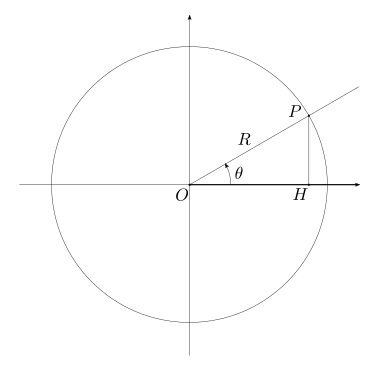
\includegraphics[width=.95\textwidth]{../../media/trigonometry-def.png}
\end{minipage}\\
\end{aligned}\end{align*}

\subsection{Relazione fondamentale della trignometria}
\label{\detokenize{ch/trigonometry:relazione-fondamentale-della-trignometria}}
\sphinxAtStartPar
Usando il teorema di Pitagora è immediato dimostrare la \sphinxstylestrong{relazione fondamentale della trigonometria} tra le funzioni seno e coseno di un angolo,
\begin{equation*}
\begin{split}\sin^2 \theta + \cos^2 \theta = 1 \ .\end{split}
\end{equation*}
\sphinxAtStartPar
\sphinxstylestrong{Nota sulla notazione.} Nell’uso delle funzioni trigonometriche, \(\sin^2 x\) indica il quadrato della funzione e non la composizione della funzione con se stessa,
\begin{equation*}
\begin{split}\sin^2 x = (\sin x)^2 \neq \sin( \sin x) \ .\end{split}
\end{equation*}

\subsection{Altre funzioni trigonometriche}
\label{\detokenize{ch/trigonometry:altre-funzioni-trigonometriche}}
\sphinxAtStartPar
\sphinxstylestrong{Tangente.} \(\tan \theta := \dfrac{\sin \theta}{\cos \theta} = \dfrac{\overline{PH}}{\overline{OH}} \ .\)

\sphinxAtStartPar
\sphinxstyleemphasis{Cosecante, secante, cotangente.} Definizioni al limite tra l’inutile e il dannoso,
\begin{equation*}
\begin{split}\begin{aligned}
  \text{cosec} \ \theta & := \frac{1}{\sin \theta} \\
  \text{sec  } \ \theta & := \frac{1}{\cos \theta} \\
  \text{cotan} \ \theta & := \frac{1}{\tan \theta} \\
\end{aligned}\end{split}
\end{equation*}

\section{Angoli particolari e proprietà}
\label{\detokenize{ch/trigonometry:angoli-particolari-e-proprieta}}\begin{equation*}
\begin{split}
\begin{minipage}[t]{.40\textwidth}
  \vspace{0pt}
  \textbf{Angoli particolari.}
  \begin{equation*}
  \begin{matrix}
   \theta & \cos \theta & \sin \theta & \tan \theta \\
   \hline 
   0             & 1                  & 0                  & 0                  \\
   \frac{\pi}{6} & \frac{\sqrt{3}}{2} & \frac{1}{2}        & \frac{1}{\sqrt{3}} \\
   \frac{\pi}{4} & \frac{\sqrt{2}}{2} & \frac{\sqrt{2}}{2} & 1                  \\
   \frac{\pi}{3} & \frac{1}{2}        & \frac{\sqrt{3}}{2} & \sqrt{3}           \\
   \frac{\pi}{2} & 0                  & 1                  & \rightarrow \infty \\
  \end{matrix}
  \end{equation*}
  \textbf{Proprietà.}
  \begin{equation*}
  \begin{aligned}
    \sin\left(-x\right)              & = - \sin x \\ 
    \cos\left(-x\right)              & =   \cos x \\ 
    \sin\left(x+\frac{\pi}{2}\right) & =   \cos x \\  
    \cos\left(x+\frac{\pi}{2}\right) & = - \sin x \\  
    \sin(x + \pi)                    & = - \sin x \\
    \cos(x + \pi)                    & = - \cos x \\
  \end{aligned}
  \end{equation*}
\end{minipage}
\hspace{.05\textwidth}
\begin{minipage}[t]{.55\textwidth}
  \vspace{0pt}
  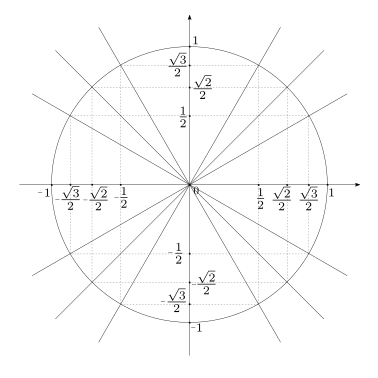
\includegraphics[width=.95\textwidth]{../../media/trigonometry-particular.png}
\end{minipage}
\end{split}
\end{equation*}

\section{Formule di somma e sottrazione}
\label{\detokenize{ch/trigonometry:formule-di-somma-e-sottrazione}}
\sphinxAtStartPar
Valgono le seguenti formule per il coseno e il seno della somma e della differenza di angoli,
\begin{equation*}
\begin{split}\begin{aligned}
  \cos ( x \mp y ) & = \cos x \ \cos y \pm \sin x \ \sin y \\
  \sin ( x \mp y ) & = \sin x \ \cos y \mp \cos x \ \sin y \\
\end{aligned}\end{split}
\end{equation*}
\sphinxAtStartPar
Per completezza, come utile esercizio di geometria sulla similitudine dei triangoli, e per familiarizzare con le funzioni armoniche, si fornisce la dimostrazione della formula del coseno della somma.
\subsubsection*{Dimostrazione di \protect\(\ \cos ( x + y ) = \cos x \ \cos y - \sin x \ \sin y\protect\)}

\begin{figure}[htbp]
\centering

\noindent\sphinxincludegraphics{{trigonometry-sum}.png}
\end{figure}

\sphinxAtStartPar
Partendo dall’interpretazione geometrica del coseno di \(\alpha + \beta\),
\begin{equation*}
\begin{split}\cos ( \alpha + \beta ) = \frac{\overline{OF}}{R}\end{split}
\end{equation*}
\sphinxAtStartPar
è necessario esprimere la lunghezza del segmento \(OF\) come multiplo del raggio \(R\).



\sphinxAtStartPar
Usando la similitudine dei triangoli \(OFE\), \(OCA\), e riconoscendo il coseno dell’angolo \(\alpha\),
\begin{equation*}
\begin{split}\overline{OF} = \frac{\overline{OC}}{\overline{OA}} \overline{OE} = \cos \alpha \ \overline{OE} \ .\end{split}
\end{equation*}
\sphinxAtStartPar
La lunghezza del segmento \(OE\) può essere scritta come differenza della lunghezza di \(OD\) e quella di \(ED\); queste ultime due lunghezze possono essere espresse come frazioni del raggio della circonferenza \(R = \overline{OB}\), grazie all’uso delle funzioni trigonometriche e alla similitudine dei triangoli (\(\overline{ED} = \sin \alpha \, \overline{BE} = \sin \alpha \, \frac{\overline{BD}}{\cos \alpha} = \sin \alpha \, \frac{\overline{OB} \sin \beta}{\cos \alpha}\)),
\begin{equation*}
\begin{split}\begin{aligned}
\overline{OE} = \overline{OD} - \overline{ED} & = \overline{OB} \cos \beta - \overline{OB} \sin \beta \frac{\sin \alpha}{\cos \alpha} = \\
& = R \left( \cos \beta - \overline{OB} \sin \beta \frac{\sin \alpha}{\cos \alpha} \right)
\end{aligned}\end{split}
\end{equation*}
\sphinxAtStartPar
Sostituendo questa espressione di \(\overline{OE}\) nell’espressione di \(\overline{OF}\), si ottiene
\begin{equation*}
\begin{split}\overline{OF} = \overline{OB} \left( \cos \alpha \cos \beta - \sin \beta \sin \alpha  \right)\end{split}
\end{equation*}
\sphinxAtStartPar
dalla quale si ottiene la relazione desiderata,
\begin{equation*}
\begin{split}\cos (\alpha + \beta) = \cos \alpha \cos \beta - \sin \beta \sin \alpha \ .\end{split}
\end{equation*}

\section{Werner}
\label{\detokenize{ch/trigonometry:werner}}\begin{equation*}
\begin{split}\begin{aligned}
  \cos x \cos y & = \dfrac{1}{2} \left[ \cos( x - y ) + \cos ( x + y ) \right] \\
  \sin x \sin y & = \dfrac{1}{2} \left[ \cos( x - y ) - \cos ( x + y ) \right] \\
  \sin x \cos y & = \dfrac{1}{2} \left[ \sin( x - y ) + \sin ( x + y ) \right] \\
\end{aligned}\end{split}
\end{equation*}\subsubsection*{Dimostrazione di \protect\(\ \cos x \cos y = \dfrac{1}{2} \left[ \cos( x - y ) + \cos ( x + y ) \right]\protect\)}

\sphinxAtStartPar
Usando le formule del coseno della somma e della sottrazione di una coppia di angoli,
\begin{equation*}
\begin{split}\begin{aligned}
  \cos( x - y ) & = \cos x \cos y + \sin x \sin y \\
  \cos( x + y ) & = \cos x \cos y - \sin x \sin y \\
\end{aligned}\end{split}
\end{equation*}
\sphinxAtStartPar
sommando termine a termine si ottiene
\begin{equation*}
\begin{split}\cos (x - y) + \cos( x + y ) = 2 \cos x \cos y \ ,\end{split}
\end{equation*}
\sphinxAtStartPar
dalla quale risulta evidente la relazione desiderata.


\section{Prostaferesi}
\label{\detokenize{ch/trigonometry:prostaferesi}}
\sphinxAtStartPar
Definendo \(p = x-y\) e \(q = x+y\) nelle formule di Werner, è immediato ricavare
\begin{equation*}
\begin{split}\begin{aligned}
  \cos p + \cos q & = 2 \cos\left(\frac{p+q}{2} \right) \cos\left(\frac{q-p}{2} \right) \\
  \cos p - \cos q & = 2 \sin\left(\frac{p+q}{2} \right) \sin\left(\frac{q-p}{2} \right) \\
  \sin p + \sin q & = 2 \sin\left(\frac{p+q}{2} \right) \cos\left(\frac{q-p}{2} \right) \\
\end{aligned}\end{split}
\end{equation*}\subsubsection*{Dimostrazione di \protect\(\ \cos p + \cos q = 2 \cos\left(\frac{p+q}{2} \right) \cos\left(\frac{q-p}{2} \right)\protect\)}

\sphinxAtStartPar
Usando la formula di Werner per il prodotto dei coseni,
\begin{equation*}
\begin{split}\cos x \cos y = \frac{1}{2} \left[ \cos(x-y) + \cos(x+y) \right]\end{split}
\end{equation*}
\sphinxAtStartPar
e definendo
\begin{equation*}
\begin{split}\begin{cases}
  x-y = p \\
  x+y = q \\
\end{cases}
\qquad \rightarrow \qquad
\begin{cases}
  2 x = p + q \\
  2 y = q - p \\
\end{cases}
\qquad \rightarrow \qquad
\begin{cases}
  x = \frac{ p + q }{2} \\
  y = \frac{ q - p }{2} \\
\end{cases}
\end{split}
\end{equation*}
\sphinxAtStartPar
si ottiene
\begin{equation*}
\begin{split}\cos \frac{p+q}{2} \cos\frac{q-p}{2} = \frac{1}{2} \left( \cos p + \cos q \right) \ ,\end{split}
\end{equation*}
\sphinxAtStartPar
dalla quale è evidente la relazione desiderata.

\sphinxstepscope


\chapter{Esponenziale e logaritmo}
\label{\detokenize{ch/exponential_logarithm:esponenziale-e-logaritmo}}\label{\detokenize{ch/exponential_logarithm:math-hs-exp-log}}\label{\detokenize{ch/exponential_logarithm::doc}}

\section{Definizioni e proprietà}
\label{\detokenize{ch/exponential_logarithm:definizioni-e-proprieta}}
\sphinxAtStartPar
Nel campo reale, per ogni \(b > 0\),
\begin{equation*}
\begin{split}a = b^c \qquad \leftrightarrow \qquad c = \log_{b} a \end{split}
\end{equation*}

\section{Funzione esponenziale e logaritmo di variabile reale}
\label{\detokenize{ch/exponential_logarithm:funzione-esponenziale-e-logaritmo-di-variabile-reale}}

\subsection{Funzione esponenziale, \protect\(e^x\protect\)}
\label{\detokenize{ch/exponential_logarithm:funzione-esponenziale-e-x}}
\sphinxAtStartPar
\sphinxstylestrong{Definizione.} Per ogni \(x \in \mathbb{R}\), è possibile dare due definizioni equivalenti della \(e^x\), che può essere intesa come l’elevamento a potenza della {\hyperref[\detokenize{ch/series:math-hs-series-e-euler}]{\sphinxcrossref{\DUrole{std,std-ref}{\(e\) di Eulero}}}} con la variabile indipendente \(x\) come esponente.
\begin{itemize}
\item {} 
\sphinxAtStartPar
definizione come limite della successione di funzioni \(\left( 1 + \frac{x}{n} \right)^n\)

\end{itemize}
\begin{equation*}
\begin{split}
  e^x := \lim_{n \rightarrow \infty} \left( 1 + \frac{x}{n}\right)^n
\end{split}
\end{equation*}\begin{itemize}
\item {} 
\sphinxAtStartPar
definizione come limite della serie di funzioni con elementi \(\frac{x^n}{n!}\),

\end{itemize}
\begin{equation*}
\begin{split}
  e^x := \lim_{n \rightarrow \infty} \sum_{k=0}^{n} \frac{x^n}{n!} \\
\end{split}
\end{equation*}
\sphinxAtStartPar
Si può dimostrare che
\begin{itemize}
\item {} 
\sphinxAtStartPar
la {\hyperref[\detokenize{ch/exponential_logarithm-proof:math-hs-exp-log-proof-convergence}]{\sphinxcrossref{\DUrole{std,std-ref}{serie è convergente}}}} per ogni \(x \in \mathbb{R}\) finito

\item {} 
\sphinxAtStartPar
le due {\hyperref[\detokenize{ch/exponential_logarithm-proof:math-hs-exp-log-proof-equivalence}]{\sphinxcrossref{\DUrole{std,std-ref}{definizioni sono equivalenti}}}}

\item {} 
\sphinxAtStartPar
le definizioni della funzione \(e^x\) giustificano la notazione \(e^x\) questa funznione poiché soddisfa le {\hyperref[\detokenize{ch/exponential_logarithm-proof:math-hs-exp-log-proof-powers}]{\sphinxcrossref{\DUrole{std,std-ref}{proprietà delle potenze (\sphinxstyleemphasis{con stessa base, \(e\)})}}}}:
\begin{equation*}
\begin{split}\begin{aligned}
    e^0 & = 1 \\
    e^1 & = e \\
  e^{x+y} & = e^x \, e^y \ .
  \end{aligned}\end{split}
\end{equation*}
\item {} 
\sphinxAtStartPar
la derivata della funzione \(e^x\) è \(e^x\), ed è una delle {\hyperref[\detokenize{ch/infinitesimal_calculus/derivatives:infinitesimal-calculus-derivatives-fund}]{\sphinxcrossref{\DUrole{std,std-ref}{derivate fondamentali}}}} del {\hyperref[\detokenize{ch/infinitesimal_calculus/derivatives:infinitesimal-calculus-derivatives}]{\sphinxcrossref{\DUrole{std,std-ref}{calcolo differenziale}}}},
\begin{equation*}
\begin{split}\frac{d}{dx} e^x = e^x \ .\end{split}
\end{equation*}
\end{itemize}



\sphinxAtStartPar
\sphinxstylestrong{Esponenziale complesso.} Si può estendere la definizione di esponenziale anche a un numero complesso, \(z \in \mathbb{C}\)
\sphinxstylestrong{todo}


\subsection{Funzione logaritmo naturale, \protect\(\text{ln} \, x\protect\)}
\label{\detokenize{ch/exponential_logarithm:funzione-logaritmo-naturale-text-ln-x}}
\sphinxAtStartPar
\sphinxstylestrong{Definizione.} Poiché la funzione \(e^x\) è monotona crescente, \(e^x: \mathbb{R} \rightarrow (0, +\infty)\), esiste la sua {\hyperref[\detokenize{ch/precalculus/real-functions:math-hs-precalculus-real-functions-inverse}]{\sphinxcrossref{\DUrole{std,std-ref}{funzione inversa}}}} con dominio \((0,+\infty)\) e immagine \(\mathbb{R}\). La funzione inversa della funzione esponenziale con base \(e\) viene definita \sphinxstylestrong{logaritmo naturale}.

\sphinxstepscope


\section{Esponenziale e logaritmo \sphinxhyphen{} dimostrazioni}
\label{\detokenize{ch/exponential_logarithm-proof:esponenziale-e-logaritmo-dimostrazioni}}\label{\detokenize{ch/exponential_logarithm-proof:math-hs-exp-log-proof}}\label{\detokenize{ch/exponential_logarithm-proof::doc}}

\subsection{Convergenza della serie di funzioni \protect\(\sum_{n=0}^{\infty} \frac{x^n}{n!}\protect\) in ogni intervallo limitato}
\label{\detokenize{ch/exponential_logarithm-proof:convergenza-della-serie-di-funzioni-sum-n-0-infty-frac-x-n-n-in-ogni-intervallo-limitato}}\label{\detokenize{ch/exponential_logarithm-proof:math-hs-exp-log-proof-convergence}}
\sphinxAtStartPar
Per dimostrare la convergenza uniforme di \(\sum_{k=0}^{\infty} \frac{x^k}{k!}\) a \(e^x\) in ogni intervallo limitato \(|x| < M\), è richiesto di dimostrare che per ogni \(\varepsilon > 0\) esiste \(N \in \mathbb{N}\) tale che
\begin{equation*}
\begin{split}|e^x - S_n(x)| < \varepsilon \ , \qquad \forall |x| < M \end{split}
\end{equation*}
\sphinxAtStartPar
per tutti gli \(n > N\). Bisogna quindi dimostrare che
\begin{equation*}
\begin{split}\left| \sum_{k=n+1}^{\infty} \frac{x^k}{k!} \right| < \varepsilon \ .\end{split}
\end{equation*}
\sphinxAtStartPar
Definendo \(\tilde{M} = \max\{ 1, M \}\)
\begin{equation*}
\begin{split}\left| \sum_{k=n+1}^{\infty} \frac{x^k}{k!} \right| < \sum_{k=n+1}^{\infty} \frac{\tilde{M}^k}{k!}\end{split}
\end{equation*}
\sphinxAtStartPar
e scegliendo \(k > 2 \tilde{M}\), in maniera da poter scrivere
\begin{equation*}
\begin{split}\frac{\tilde{M}^k}{k!} = \frac{\tilde{M}^{2 \tilde{M}}}{( 2 \tilde{M})!} \frac{\tilde{M}}{2\tilde{M}+1} \dots \frac{\tilde{M}}{k} <  \frac{\tilde{M}^{2 \tilde{M}}}{( 2 \tilde{M})!} 2^{-(k - \tilde{M})} = \frac{(2 \tilde{M})^{2 \tilde{M}}}{(2 \tilde{M})!} 2^{-k}\end{split}
\end{equation*}
\sphinxAtStartPar
e quindi
\begin{equation*}
\begin{split}\sum_{k=n+1}^{\infty} \frac{\tilde{M}}{k!} < \sum_{k=n+1}^{\infty} \frac{(2 \tilde{M})^{2 \tilde{M}}}{(2\tilde{M})!} 2^{-k} =  \frac{(2 \tilde{M})^{2 \tilde{M}}}{(2\tilde{M})!} 2^{-n}\end{split}
\end{equation*}
\sphinxAtStartPar
avendo usato \(\sum_{k=n+1}^{\infty} 2^{-k} = 2^{-n-1} \sum_{k=0}^{\infty} 2^{-k} = 2^{-n-1} \cdot 2 = 2^{-n}\).
Scegliendo \(N > \log_2 \left( \frac{1}{\varepsilon} \frac{(2\tilde{M})^{2 \tilde{M}}}{(2 \tilde{M})!)} \right)\), per ogni \(n > N\) si ha
\begin{equation*}
\begin{split}\left| \sum_{k=n+1}^{\infty} \frac{x^k}{k!} \right| <  \frac{(2 \tilde{M})^{2 \tilde{M}}}{(2\tilde{M})!} 2^{-n} <  \frac{(2 \tilde{M})^{2 \tilde{M}}}{(2\tilde{M})!} 2^{-N} < \varepsilon \ .\end{split}
\end{equation*}



\subsection{Equivalenza delle due definizioni}
\label{\detokenize{ch/exponential_logarithm-proof:equivalenza-delle-due-definizioni}}\label{\detokenize{ch/exponential_logarithm-proof:math-hs-exp-log-proof-equivalence}}
\sphinxAtStartPar
\sphinxstylestrong{todo}


\subsection{Giustificazione della notazione \protect\(\ e^x\protect\)}
\label{\detokenize{ch/exponential_logarithm-proof:giustificazione-della-notazione-e-x}}\label{\detokenize{ch/exponential_logarithm-proof:math-hs-exp-log-proof-powers}}
\sphinxAtStartPar
Per evitare la forma indeterminata nel termine \(0^0\), si calcola qui il limite per \(x \rightarrow 0\) (\sphinxstylestrong{todo} \sphinxstyleemphasis{motivare la validità di questa operazione/interpretazione della funzione \(e^x\)})
\begin{equation*}
\begin{split}e^0 := \lim_{x \rightarrow 0} e^x = \lim_{x \rightarrow 0} \sum_{n = 0}^{\infty} \frac{x^n}{n!} = 1 + \lim_{x \rightarrow 0} \sum_{n=1}^{\infty} \frac{x^n}{n!} = 1 \ .\end{split}
\end{equation*}
\sphinxAtStartPar
Ricordando la definizione della \(e\) di Eulero, è immediato verificare che il valore della serie di funzioni per \(x = 1\) coincide con il valore di \(e\)
\begin{equation*}
\begin{split}e^1 = \sum_{n=0}^{\infty} \frac{x^n}{n!} \bigg|_{x=1} = \sum_{n=0}^{\infty} \frac{1}{n!} = e \ .\end{split}
\end{equation*}
\sphinxAtStartPar
La serie che definisce la esponenziale soddisfa la proprietà delle potenze \(e^x \, e^y = e^{x+y}\),
\begin{equation*}
\begin{split}\begin{aligned}
  e^x \, e^y 
  & = \sum_{n=0}^{\infty} \frac{x^n}{n!} \sum_{m = 0}^{\infty} \frac{y^m}{m!} = \\
  & = \sum_{n=0}^{\infty} \sum_{m=0}^{\infty} \frac{y^m}{m!} \frac{x^n}{n!} =  & \text{($m,n \  \rightarrow \ m,p=m+n$)}\\
  & = \sum_{p=0}^{\infty} \sum_{m=0}^{p} \frac{y^m \, x^{p-m}}{m! (p-m!)} = \\
  & = \sum_{p=0}^{\infty} \frac{1}{p!} \underbrace{\sum_{m=0}^{p} \frac{p!}{m! (p-m)!} y^m \, x^{p-m}}_{(x+y)^p} = \\
  & = \sum_{p=0}^{\infty} \frac{(x+y)^p}{p!} = \\
  & = e^{x+y} \ ,
\end{aligned}\end{split}
\end{equation*}
\sphinxAtStartPar
avendo usato il {\hyperref[\detokenize{ch/precalculus/polynomials:math-hs-precalculus-polynomials-binomial-thm}]{\sphinxcrossref{\DUrole{std,std-ref}{teorema binomiale}}}}.

\sphinxstepscope

\begin{sphinxuseclass}{sd-container-fluid}
\begin{sphinxuseclass}{sd-sphinx-override}
\begin{sphinxuseclass}{sd-p-0}
\begin{sphinxuseclass}{sd-mt-2}
\begin{sphinxuseclass}{sd-mb-4}
\begin{sphinxuseclass}{sd-row}
\begin{sphinxuseclass}{sd-row-cols-2}
\begin{sphinxuseclass}{sd-gx-2}
\begin{sphinxuseclass}{sd-gy-1}
\begin{sphinxuseclass}{sd-col}
\begin{sphinxuseclass}{sd-d-flex-row}
\begin{sphinxuseclass}{sd-align-minor-center}
\begin{sphinxuseclass}{sd-container-fluid}
\begin{sphinxuseclass}{sd-sphinx-override}
\begin{sphinxuseclass}{sd-row}
\begin{sphinxuseclass}{sd-row-cols-2}
\begin{sphinxuseclass}{sd-row-cols-xs-2}
\begin{sphinxuseclass}{sd-row-cols-sm-3}
\begin{sphinxuseclass}{sd-row-cols-md-3}
\begin{sphinxuseclass}{sd-row-cols-lg-3}
\begin{sphinxuseclass}{sd-gx-3}
\begin{sphinxuseclass}{sd-gy-1}
\begin{sphinxuseclass}{sd-col}
\begin{sphinxuseclass}{sd-col-auto}
\begin{sphinxuseclass}{sd-d-flex-row}
\begin{sphinxuseclass}{sd-align-minor-center}
\sphinxAtStartPar
basics

\end{sphinxuseclass}
\end{sphinxuseclass}
\end{sphinxuseclass}
\end{sphinxuseclass}
\begin{sphinxuseclass}{sd-col}
\begin{sphinxuseclass}{sd-col-auto}
\begin{sphinxuseclass}{sd-d-flex-row}
\begin{sphinxuseclass}{sd-align-minor-center}
\sphinxAtStartPar
Nov 10, 2024

\end{sphinxuseclass}
\end{sphinxuseclass}
\end{sphinxuseclass}
\end{sphinxuseclass}
\begin{sphinxuseclass}{sd-col}
\begin{sphinxuseclass}{sd-col-auto}
\begin{sphinxuseclass}{sd-d-flex-row}
\begin{sphinxuseclass}{sd-align-minor-center}
\sphinxAtStartPar
0 min read

\end{sphinxuseclass}
\end{sphinxuseclass}
\end{sphinxuseclass}
\end{sphinxuseclass}
\end{sphinxuseclass}
\end{sphinxuseclass}
\end{sphinxuseclass}
\end{sphinxuseclass}
\end{sphinxuseclass}
\end{sphinxuseclass}
\end{sphinxuseclass}
\end{sphinxuseclass}
\end{sphinxuseclass}
\end{sphinxuseclass}
\end{sphinxuseclass}
\end{sphinxuseclass}
\end{sphinxuseclass}
\end{sphinxuseclass}
\end{sphinxuseclass}
\end{sphinxuseclass}
\end{sphinxuseclass}
\end{sphinxuseclass}
\end{sphinxuseclass}
\end{sphinxuseclass}
\end{sphinxuseclass}
\end{sphinxuseclass}

\chapter{Funzioni multi\sphinxhyphen{}variabile}
\label{\detokenize{ch/precalculus/multivariable-real-fun:funzioni-multi-variabile}}\label{\detokenize{ch/precalculus/multivariable-real-fun:math-hs-precalculus-multivariable-real-fun}}\label{\detokenize{ch/precalculus/multivariable-real-fun::doc}}
\sphinxstepscope


\part{Calcolo}

\sphinxstepscope

\begin{sphinxuseclass}{sd-container-fluid}
\begin{sphinxuseclass}{sd-sphinx-override}
\begin{sphinxuseclass}{sd-p-0}
\begin{sphinxuseclass}{sd-mt-2}
\begin{sphinxuseclass}{sd-mb-4}
\begin{sphinxuseclass}{sd-row}
\begin{sphinxuseclass}{sd-row-cols-2}
\begin{sphinxuseclass}{sd-gx-2}
\begin{sphinxuseclass}{sd-gy-1}
\begin{sphinxuseclass}{sd-col}
\begin{sphinxuseclass}{sd-d-flex-row}
\begin{sphinxuseclass}{sd-align-minor-center}
\begin{sphinxuseclass}{sd-container-fluid}
\begin{sphinxuseclass}{sd-sphinx-override}
\begin{sphinxuseclass}{sd-row}
\begin{sphinxuseclass}{sd-row-cols-2}
\begin{sphinxuseclass}{sd-row-cols-xs-2}
\begin{sphinxuseclass}{sd-row-cols-sm-3}
\begin{sphinxuseclass}{sd-row-cols-md-3}
\begin{sphinxuseclass}{sd-row-cols-lg-3}
\begin{sphinxuseclass}{sd-gx-3}
\begin{sphinxuseclass}{sd-gy-1}
\begin{sphinxuseclass}{sd-col}
\begin{sphinxuseclass}{sd-col-auto}
\begin{sphinxuseclass}{sd-d-flex-row}
\begin{sphinxuseclass}{sd-align-minor-center}
\sphinxAtStartPar
basics

\end{sphinxuseclass}
\end{sphinxuseclass}
\end{sphinxuseclass}
\end{sphinxuseclass}
\begin{sphinxuseclass}{sd-col}
\begin{sphinxuseclass}{sd-col-auto}
\begin{sphinxuseclass}{sd-d-flex-row}
\begin{sphinxuseclass}{sd-align-minor-center}
\sphinxAtStartPar
Nov 10, 2024

\end{sphinxuseclass}
\end{sphinxuseclass}
\end{sphinxuseclass}
\end{sphinxuseclass}
\begin{sphinxuseclass}{sd-col}
\begin{sphinxuseclass}{sd-col-auto}
\begin{sphinxuseclass}{sd-d-flex-row}
\begin{sphinxuseclass}{sd-align-minor-center}
\sphinxAtStartPar
2 min read

\end{sphinxuseclass}
\end{sphinxuseclass}
\end{sphinxuseclass}
\end{sphinxuseclass}
\end{sphinxuseclass}
\end{sphinxuseclass}
\end{sphinxuseclass}
\end{sphinxuseclass}
\end{sphinxuseclass}
\end{sphinxuseclass}
\end{sphinxuseclass}
\end{sphinxuseclass}
\end{sphinxuseclass}
\end{sphinxuseclass}
\end{sphinxuseclass}
\end{sphinxuseclass}
\end{sphinxuseclass}
\end{sphinxuseclass}
\end{sphinxuseclass}
\end{sphinxuseclass}
\end{sphinxuseclass}
\end{sphinxuseclass}
\end{sphinxuseclass}
\end{sphinxuseclass}
\end{sphinxuseclass}
\end{sphinxuseclass}

\chapter{Introduzione al calcolo}
\label{\detokenize{ch/calculus:introduzione-al-calcolo}}\label{\detokenize{ch/calculus:math-hs-calculus}}\label{\detokenize{ch/calculus::doc}}
\sphinxAtStartPar
Il calcolo si occupa della variazione continua di grandezze matematiche che possono essere rappresentate come funzioni di variabili indipendenti.

\sphinxAtStartPar
Gli strumenti matematici del calcolo vengono sviluppati e formalizzati tra la fine del XVII secolo e il XIX secolo, come strumenti necessari alla costruzione delle teorie fisiche della meccanica razionale di Newton prima, e della meccanica dei mezzi continui (fluidi e solidi) poi.

\sphinxAtStartPar
Newton introduce i concetti fondamentali calcolo differenziale e integrale delle funzioni di una variabile, qui chiamato {\hyperref[\detokenize{ch/infinitesimal_calculus:infinitesimal-calculus}]{\sphinxcrossref{\DUrole{std,std-ref}{calcolo infinitesimale}}}}, necessari allo sviluppo della meccanica: nella meccanica di Newton, il moto di un sistema meccanico è descritto dai suoi gradi di libertà in funzione della variabile tempo, e le equazioni che ne governano il moto sono equazioni differenziali ordinarie. Il lavoro di Newton, e il lavoro contemporaneo di Leibniz, parte dalla {\hyperref[\detokenize{ch/analytic_geometry:geometry-analytic}]{\sphinxcrossref{\DUrole{std,std-ref}{geometria analitica}}}}, che permette di associare una curva a una funzione, e sviluppa la risposta ad alcuni problemi riguardanti la geometria delle curve, come il calcolo della tangente a una curva, la ricerca dei minimi e dei massimi di una funzione o il calcolo delle aree.

\sphinxAtStartPar
I risultati del calcolo differenziale e integrale vengono connessi tra di loro dal \sphinxstylestrong{teorema fondamentale del calcolo} (\sphinxstylestrong{todo} aggiungere riferimento).

\sphinxAtStartPar
A Eulero si deve una prima raccolta degli strumenti utili a un’introduzione al calcolo, come discusso nel capitolo sul {\hyperref[\detokenize{ch/precalculus:math-hs-precalculus}]{\sphinxcrossref{\DUrole{std,std-ref}{precalcolo}}}}.

\sphinxAtStartPar
Al lavoro di Johann e Jakob Bernoulli e ancora Eulero si deve l’ideazione del calcolo delle variazioni (\sphinxstylestrong{todo} \sphinxstyleemphasis{aggiungere una sezione?}), ampiamente sviluppato da \sphinxstylestrong{Lagrange} nella sua riformulazione geometrica della meccanica.

\sphinxAtStartPar
Nel corso del XVIII e del XIX secolo, il calcolo infinitesimale si sviluppo come lo strumento matematico indispensabile nei problemi di fisica: Lagrange introduce il concetto di potenziale in meccanica, mentre Green sviluppa gli strumenti del calcolo infinitesimale per funzioni di più variabili (teorema di Green, estensione del rotore allo spazio 3\sphinxhyphen{}dimensionale, metodo della funzione di Green) nel suo “Saggio sull’Applicazione della Analisi Matematica alle Teorie dell’Elettricità e del Magnetismo” del 1828, testo “in anticipo di 30 anni rispetto al suo tempo” secondo Einstein, ma rimasto a lungo trascurato.

\sphinxAtStartPar
Nel XIX secolo Gauss contribuì allo sviluppo del calcolo multivariabile applicato allo studio delle curve e delle superfici, e alla teoria matematica dell’elettromagnetismo.

\sphinxAtStartPar
Nel XIX secolo il calcolo infinitesimale si impose come strumento matematico fondamentale in diversi ambiti:
\begin{itemize}
\item {} 
\sphinxAtStartPar
meccanica dei solidi e dei fluidi:

\item {} 
\sphinxAtStartPar
diffusione del calore per conduzione

\item {} 
\sphinxAtStartPar
elettromagnetismo

\end{itemize}

\sphinxAtStartPar
Cauchy diede importanti contributi allo sviluppo del calcolo complesso, successivamente sviluppato da Riemann.

\sphinxAtStartPar
Cauchy contribuì inoltre alla definizione rigorosa dei fondamenti del calcolo, portata avanti da Weierstrass nella seconda metà del XIX secolo con la definizione di limite e continuità di una funzione.



\sphinxstepscope


\chapter{Calcolo infinitesimale}
\label{\detokenize{ch/infinitesimal_calculus:calcolo-infinitesimale}}\label{\detokenize{ch/infinitesimal_calculus:infinitesimal-calculus}}\label{\detokenize{ch/infinitesimal_calculus::doc}}
\sphinxAtStartPar
Il calcolo infinitesimale si occupa dello studio \sphinxstyleemphasis{delle variazioni con continuità delle grandezze} \sphinxstylestrong{todo}.

\sphinxAtStartPar
Questo capitolo presenta il calcolo infinitesimale per le funzioni reali di una variabile reale, \(f: D \in \mathbb{R} \rightarrow \mathbb{R}\), come inizialmente formulate da Newton e Lebniz alla fine del XVII secolo nell’ambito dello sviluppo della \sphinxhref{https://basics2022.github.io/bbooks-physics-hs/ch/mechanics.html}{meccanica classica}, e successivamente formalizzate nel XIX secolo grazie all’opera, tra gli altri, di Cauchy e Weierstrass. Infine vengono introdotte le equazioni differenziali ordinarie. \sphinxstylestrong{todo} \sphinxstyleemphasis{due parole sull’importanza delle equazioni differenziali?}

\sphinxAtStartPar
La presentazione degli argomenti è invertita rispetto a questo ordine cronologico per rispettare un ordine logico: prima vengono presentati alcuni fondamenti dell’\sphinxstylestrong{analisi}, come sviluppati da Cauchy e Weierstrass nel XIX secolo; successivamente, questi concetti vengono utilizzati per definire e dare fondamento teorico ai concetti del \sphinxstylestrong{calcolo differenziale} e \sphinxstylestrong{integrale}, introdotti più di un secolo prima da Newton e Leibniz partendo da risultati di geometria analitica.



\sphinxAtStartPar
\sphinxstylestrong{Argomenti del capitolo.}
\begin{itemize}
\item {} 
\sphinxAtStartPar
{\hyperref[\detokenize{ch/infinitesimal_calculus/analysis:infinitesimal-calculus-analysis}]{\sphinxcrossref{\DUrole{std,std-ref}{\sphinxstylestrong{Introduzione all’analisi}}}}}. Viene richiamato il concetto di \sphinxstylestrong{funzione} di variabile reale a valore reale, \(f: D \in \mathbb{R} \rightarrow \mathbb{R}\), e la sua rappresentazione grafica in un piano cartesiano.

\sphinxAtStartPar
Viene introdotto il concetto di \sphinxstylestrong{limite} per funzioni reali e viene usato per definire le \sphinxstylestrong{funzioni continue}. Vengono quindi presentati alcuni teoremi sulle funzioni continue e sui limiti che ne permettono il calcolo. Vengono presentate le forme indeterminate al finito e all’infinito, e calcolati i \sphinxstyleemphasis{limiti fondamentali}.

\item {} 
\sphinxAtStartPar
{\hyperref[\detokenize{ch/infinitesimal_calculus/derivatives:infinitesimal-calculus-derivatives}]{\sphinxcrossref{\DUrole{std,std-ref}{\sphinxstylestrong{Calcolo differenziale}}}}}. Usando i concetti di limite della sezione precedente, viene introdotto il concetto di \sphinxstylestrong{derivata} di una funzione reale, e viene data una sua interpretazione geometrica, legata alla retta tangente al grafico della funzione. Seguono alcune proprietà e teoremi sulle derivate che permettono di valutare le \sphinxstyleemphasis{derivate fondamentali} e combinare questi risultati per il calcolo della derivata di una funzione qualsiasi. Infine viene introdotto il concetto di derivate di ordine superiore, e vengono mostrate alcune applicazioni: ricerca di punti di estremo locale e di flesso nello studio di funzione, ottimizzazione, approssimazione locale tramite sviluppi in serie polinomiali

\item {} 
\sphinxAtStartPar
{\hyperref[\detokenize{ch/infinitesimal_calculus/integrals:infinitesimal-calculus-integrals}]{\sphinxcrossref{\DUrole{std,std-ref}{\sphinxstylestrong{Calcolo integrale}}}}}. Viene data la definizione di \sphinxstylestrong{integrale di Riemann} e una sua interpretazione geometrica, legata all’area sottesa dal grafico della funzione. Seguono alcune proprietà degli integrali che permettono di definire l’integrale definito e indefinito, e la primitiva di una funzione. Viene presentato il \sphinxstylestrong{teorema fondamentale del calcolo infinitesimale}, che permette di riconoscere l’operazione di integrazione come inversa dell’integrazione. Usando questo risultato, vengono valutati gli \sphinxstyleemphasis{integrali fondamentali}; poche regole di integrazione permettono poi di calcolare l’integrale di funzioni generiche. Infine vengono mostrate alcune applicazioni: … \sphinxstylestrong{todo}

\item {} 
\sphinxAtStartPar
{\hyperref[\detokenize{ch/ode:ode-hs}]{\sphinxcrossref{\DUrole{std,std-ref}{\sphinxstylestrong{Equazioni differenziali ordinarie}}}}}. \sphinxstylestrong{todo}

\end{itemize}



\sphinxstepscope


\section{Introduzione all’analisi}
\label{\detokenize{ch/infinitesimal_calculus/analysis:introduzione-all-analisi}}\label{\detokenize{ch/infinitesimal_calculus/analysis:infinitesimal-calculus-analysis}}\label{\detokenize{ch/infinitesimal_calculus/analysis::doc}}
\sphinxAtStartPar
In questa sezione viene richiamato il concetto di funzione introdotto nella sezione {\hyperref[\detokenize{ch/precalculus:math-hs-precalculus}]{\sphinxcrossref{\DUrole{std,std-ref}{Precalcolo}}}}. Viene introdotto il concetto di {\hyperref[\detokenize{ch/infinitesimal_calculus/analysis:infinitesimal-calculus-limits}]{\sphinxcrossref{\DUrole{std,std-ref}{limite}}}} e definito in termini topologici (intervalli, punti di accumulazione, insiemi aperti e chiusi,…). Il concetto di limite viene utilizzato per dare una definizione di {\hyperref[\detokenize{ch/infinitesimal_calculus::doc}]{\sphinxcrossref{\DUrole{doc,std,std-doc}{funzione continua}}}}. Vengono poi presentati alcuni teoremi e proprietà di limiti e funzioni continue.




\subsection{Funzioni reali a variabile reale, \protect\(f: \mathbb{R} \rightarrow \mathbb{R}\protect\)}
\label{\detokenize{ch/infinitesimal_calculus/analysis:funzioni-reali-a-variabile-reale-f-mathbb-r-rightarrow-mathbb-r}}\label{\detokenize{ch/infinitesimal_calculus/analysis:infinitesimal-calculus-analysis-real-functions}}

\subsubsection{Definizione}
\label{\detokenize{ch/infinitesimal_calculus/analysis:definizione}}\label{\detokenize{ch/infinitesimal_calculus/analysis:infinitesimal-calculus-analysis-real-functions-def}}

\subsubsection{Rappresentazione grafica}
\label{\detokenize{ch/infinitesimal_calculus/analysis:rappresentazione-grafica}}\label{\detokenize{ch/infinitesimal_calculus/analysis:infinitesimal-calculus-analysis-real-functions-graph}}



\subsection{Limiti}
\label{\detokenize{ch/infinitesimal_calculus/analysis:limiti}}\label{\detokenize{ch/infinitesimal_calculus/analysis:infinitesimal-calculus-limits}}

\subsubsection{Cenni di topologia per il calcolo}
\label{\detokenize{ch/infinitesimal_calculus/analysis:cenni-di-topologia-per-il-calcolo}}
\sphinxAtStartPar
\sphinxstylestrong{todo} \sphinxstyleemphasis{Punto di accumulazione e punto isolato, intorno, insiemi aperti e chiusi, limsup/liminf, max/min,… E’ necessario? Il minimo indispensabile}


\subsubsection{Definizione di limite}
\label{\detokenize{ch/infinitesimal_calculus/analysis:definizione-di-limite}}\label{\detokenize{ch/infinitesimal_calculus/analysis:infinitesimal-calculus-limits-def}}


\sphinxAtStartPar
\sphinxstylestrong{Limite finito al finito}
\begin{equation*}
\begin{split}\forall \varepsilon > 0 \quad \exists U_{x_0,\delta} \quad {t.c.} \quad |f(x) - L| < \varepsilon \quad \forall x \in U_{x_0, \delta} \backslash \{x_0\}\end{split}
\end{equation*}
\sphinxAtStartPar
dove la condizione sull’intorno di un punto \(x_0\) al finito per funzioni reali può essere riscritta come \(0 < | x - x_0 | <  \delta\) per un intorno simmetrico del punto \(x_0\).

\sphinxAtStartPar
\sphinxstylestrong{Limite infinito al finito}
\begin{equation*}
\begin{split}\forall M > 0 \quad \exists U_{x_0,\delta} \quad {t.c.} \quad |f(x)| > M \quad \forall x \in U_{x_0, \delta} \backslash \{x_0\}\end{split}
\end{equation*}
\sphinxAtStartPar
dove la condizione sull’intorno di un punto \(x_0\) al finito per funzioni reali può essere riscritta come \(0 < | x - x_0 | <  \delta\) per un intorno simmetrico del punto \(x_0\). Se \(f(x) > M\) allora il limite tende a \(+\infty\), se \(f(x) < -M\) allora il limite tende a \(-\infty\).

\sphinxAtStartPar
\sphinxstylestrong{Limite finito all’infinito}
\begin{equation*}
\begin{split}\forall \varepsilon > 0 \quad \exists U_{\mp\infty,R} \quad {t.c.} \quad |f(x) - L| < \varepsilon \quad \forall x \in U_{\mp\infty, R}\end{split}
\end{equation*}
\sphinxAtStartPar
dove la condizione sull’intorno di un punto all’infinito per funzioni reali può essere riscritta come \(x < R\) per un intorno di \(-\infty\) o \(x > R\) per un intorno di \(+\infty\).

\sphinxAtStartPar
\sphinxstylestrong{Limite infinito all’infinito}
\begin{equation*}
\begin{split}\forall M > 0 \quad \exists U_{\mp \infty, R} \quad {t.c.} \quad |f(x)| > M \quad \forall x \in U_{\mp \infty, R}\end{split}
\end{equation*}
\sphinxAtStartPar
dove la condizione sull’intorno di un punto all’infinito per funzioni reali può essere riscritta come \(x < R\) per un intorno di \(-\infty\) o \(x > R\) per un intorno di \(+\infty\). Se \(f(x) > M\) allora il limite tende a \(+\infty\), se \(f(x) < -M\) allora il limite tende a \(-\infty\).


\subsection{Funzioni continue}
\label{\detokenize{ch/infinitesimal_calculus/analysis:funzioni-continue}}\label{\detokenize{ch/infinitesimal_calculus/analysis:infinitesimal-calculus-continuous-fun}}

\subsubsection{Definizione}
\label{\detokenize{ch/infinitesimal_calculus/analysis:infinitesimal-calculus-continuous-fun-def}}\label{\detokenize{ch/infinitesimal_calculus/analysis:id1}}
\sphinxAtStartPar
Una funzione reale \(f: D \in \mathbb{R} \rightarrow \mathbb{R}\) è continua in un punto \(x_0 \in D\) se la funzione è definita nel punto, se esiste il limite della fuzione e coincide con il valore della funzione
\begin{equation*}
\begin{split}\lim_{x \rightarrow x_0} f(x) = f(x_0) \ .\end{split}
\end{equation*}
\sphinxAtStartPar
Una funzione reale è continua in un dominio \sphinxstylestrong{todo o insieme?} se è continua in ogni punto del dominio.


\subsubsection{Teoremi}
\label{\detokenize{ch/infinitesimal_calculus/analysis:teoremi}}\label{\detokenize{ch/infinitesimal_calculus/analysis:infinitesimal-calculus-continuous-fun-thms}}

\paragraph{Teorema di Weierstrass}
\label{\detokenize{ch/infinitesimal_calculus/analysis:teorema-di-weierstrass}}\label{\detokenize{ch/infinitesimal_calculus/analysis:infinitesimal-calculus-continuous-fun-thms-weierstrass}}
\sphinxAtStartPar
Data una funzione reale continua \(f: [a,b] \rightarrow \mathbb{R}\) definita sull’intervallo chiuso \([a,b]\), la funzione \(f(x)\) ammette un punto di massimo assoluto e un punto di minimo assoluto nell’intevallo \([a,b]\).

\sphinxAtStartPar
\sphinxstylestrong{todo} \sphinxstyleemphasis{Dimostrazione? Discussione più intuitiva? Figura?}


\paragraph{Teorema della permanenza del segno}
\label{\detokenize{ch/infinitesimal_calculus/analysis:teorema-della-permanenza-del-segno}}\label{\detokenize{ch/infinitesimal_calculus/analysis:infinitesimal-calculus-continuous-fun-thms-sign}}
\sphinxAtStartPar
Data una funzione continua \(f: D \rightarrow \mathbb{R}\) continua, e un punto \(x_0 \in D\). Se \(f(x_0) > 0\) allora \(\exists U_{x_0}\) t.c. \(f(x) > 0\) per \(\forall x \in U_{x_0} \cap D\).

\sphinxAtStartPar
\sphinxstylestrong{todo} \sphinxstyleemphasis{Dimostrazione? Discussione più intuitiva? Figura?}


\paragraph{Teorema dei valori intermedi}
\label{\detokenize{ch/infinitesimal_calculus/analysis:teorema-dei-valori-intermedi}}\label{\detokenize{ch/infinitesimal_calculus/analysis:infinitesimal-calculus-continuous-fun-thms-intermediate}}
\sphinxAtStartPar
Data una funzione \(f: [a,b] \rightarrow \mathbb{R}\) continua, allora \(f(x)\) assume tutti i valori compresi tra \(f(a)\) e \(f(b)\), cioè (assumendo \(f(a) < f(b)\)) per \(\forall y \in (f(a), f(b)) \ x_0 \in (a,b) \ \text{t.c..} \ f(x_0) = y\).

\sphinxAtStartPar
\sphinxstylestrong{todo} \sphinxstyleemphasis{Dimostrazione? Discussione più intuitiva? Figura?}


\subsection{Teoremi sui limiti}
\label{\detokenize{ch/infinitesimal_calculus/analysis:teoremi-sui-limiti}}\label{\detokenize{ch/infinitesimal_calculus/analysis:infinitesimal-calculus-limits-thms}}

\subsubsection{Operazioni coi limiti}
\label{\detokenize{ch/infinitesimal_calculus/analysis:operazioni-coi-limiti}}\label{\detokenize{ch/infinitesimal_calculus/analysis:infinitesimal-calculus-limits-thms-operations}}
\sphinxAtStartPar
Dato un numero reale \(c \in \mathbb{R}\) e i limiti \(\lim_{x \rightarrow x_0} f(x) = L_1\), \(\lim_{x \rightarrow x_0} g(x) = L_2\)
\begin{equation*}
\begin{split}\begin{aligned}
 & \lim_{x \rightarrow x_0} \big( c \cdot f(x) \big) = c \, L_1 \\
 & \lim_{x \rightarrow x_0} \big( f(x) \mp g(x) \big) = L_1 \mp L_2 \\
 & \lim_{x \rightarrow x_0} \big( f(x) \cdot g(x) \big) = L_1 \cdot L_2 \\
 & \lim_{x \rightarrow x_0} \frac{ f(x) }{ g(x) } = \frac{L_1}{L_2} \quad , \quad \text{se $L_2 \ne 0$}  \\
\end{aligned}\end{split}
\end{equation*}

\paragraph{Limiti infiniti e infinitesimi}
\label{\detokenize{ch/infinitesimal_calculus/analysis:limiti-infiniti-e-infinitesimi}}\label{\detokenize{ch/infinitesimal_calculus/analysis:infinitesimal-calculus-limits-thms-infinite-simal}}\begin{equation*}
\begin{split}\begin{aligned}
 &  \lim_{x \rightarrow x_0}f(x) \rightarrow \mp \infty \ , c > 0 \quad : \qquad \lim_{x \rightarrow x_0} c \cdot f(x) = \mp \infty \\
 & \dots \\
\end{aligned}\end{split}
\end{equation*}

\paragraph{Forme indeterminate}
\label{\detokenize{ch/infinitesimal_calculus/analysis:forme-indeterminate}}\label{\detokenize{ch/infinitesimal_calculus/analysis:infinitesimal-calculus-limits-thms-infinite-simal-undetermined}}\begin{equation*}
\begin{split}+\infty-\infty \quad , \quad 0 \cdot \mp \infty \quad , \quad \frac{\mp \infty}{\mp \infty} \quad , \quad \frac{0}{0} \quad , \quad 1^{\infty} \quad , \quad 0^0 \quad , \quad \infty^0\end{split}
\end{equation*}
\sphinxAtStartPar
\sphinxstylestrong{oss.} Invece non sono forme indeterminate \(0^{+\infty} \rightarrow 0\) e \(0^{-\infty} \rightarrow \infty\).


\subsubsection{Teorema del confronto}
\label{\detokenize{ch/infinitesimal_calculus/analysis:teorema-del-confronto}}\label{\detokenize{ch/infinitesimal_calculus/analysis:infinitesimal-calculus-limits-thms-comparison}}
\sphinxAtStartPar
Siano \(f\), \(g\), \(h: \ X \in \mathbb{R} \rightarrow \mathbb{R}\), e dato un punto di accumulazione \(x_0\) per \(X\). Se
\begin{equation*}
\begin{split}\lim_{x \rightarrow x_0} f(x) = \lim_{x \rightarrow x_0} h(x) = \ell \ ,\end{split}
\end{equation*}
\sphinxAtStartPar
ed esiste un intorno \(U\) di \(x_0\) tale che
\begin{equation*}
\begin{split}f(x) \le g(x) \le h(x) \quad \forall x \in U \cap X \ \{ x_0 \} \ ,\end{split}
\end{equation*}
\sphinxAtStartPar
allora
\begin{equation*}
\begin{split}\lim_{x \rightarrow x_0} g(x) = \ell \ .\end{split}
\end{equation*}
\sphinxAtStartPar
\sphinxstylestrong{todo} \sphinxstyleemphasis{Dimostrazione? Discussione più intuitiva? Figura?}


\subsubsection{Teorema di de l’Hopital}
\label{\detokenize{ch/infinitesimal_calculus/analysis:teorema-di-de-l-hopital}}\label{\detokenize{ch/infinitesimal_calculus/analysis:infinitesimal-calculus-limits-thms-hopital}}
\sphinxAtStartPar
Il teorema di de l’Hopital (o di Bernoulli, \sphinxstylestrong{todo} \sphinxstyleemphasis{dire due parole sulla storia? Bernoulli precettore di de l’Hopital, ricava il risultato…}) è un teorema utile per il calcolo dei limiti delle forme indeterminate \(\frac{0}{0}\) e \(\frac{\infty}{\infty}\). Poiché il teorema coinvolge il concetto di derivata, si rimanda alla sezione del {\hyperref[\detokenize{ch/infinitesimal_calculus/derivatives:infinitesimal-calculus-derivatives-thm-hopital}]{\sphinxcrossref{\DUrole{std,std-ref}{teorema di de l’Hopital}}}} nel capitolo sulle {\hyperref[\detokenize{ch/infinitesimal_calculus/derivatives:infinitesimal-calculus-derivatives}]{\sphinxcrossref{\DUrole{std,std-ref}{derivate}}}}.


\subsection{Limiti fondamentali}
\label{\detokenize{ch/infinitesimal_calculus/analysis:limiti-fondamentali}}\label{\detokenize{ch/infinitesimal_calculus/analysis:infinitesimal-calculus-limits-fund}}
\sphinxAtStartPar
In questa sezione vengono calcolati alcuni limiti fondamentali. Questi limiti possono essere considerati fondamentali come sinonimo di \sphinxstyleemphasis{“minimo da ricordare”} per poter calcolare limiti più generali utilizzando le {\hyperref[\detokenize{ch/infinitesimal_calculus/analysis:infinitesimal-calculus-limits-thms-operations}]{\sphinxcrossref{\DUrole{std,std-ref}{operazioni}}}} e i {\hyperref[\detokenize{ch/infinitesimal_calculus/analysis:infinitesimal-calculus-limits-thms}]{\sphinxcrossref{\DUrole{std,std-ref}{teoremi}}}} sui limiti, e calcolare le {\hyperref[\detokenize{ch/infinitesimal_calculus/derivatives:infinitesimal-calculus-derivatives-fund}]{\sphinxcrossref{\DUrole{std,std-ref}{derivate fondamentali}}}}. Un elenco minimo di limiti fondamentali è:
\begin{equation*}
\begin{split} \lim_{x \rightarrow 0} \frac{(1+x)^a - 1}{x} = a \end{split}
\end{equation*}\begin{equation*}
\begin{split} \lim_{x \rightarrow 0} \frac{\sin x}{x} = 1 \end{split}
\end{equation*}\begin{equation*}
\begin{split} \lim_{x \rightarrow 0} \frac{1 - \cos^2 x}{x^2} = \frac{1}{2} \end{split}
\end{equation*}\begin{equation*}
\begin{split} \lim_{x \rightarrow +\infty} \left( 1 + \frac{1}{x} \right)^x = e \end{split}
\end{equation*}\begin{equation*}
\begin{split} \lim_{x \rightarrow 0} \frac{e^x - 1}{x}= 1 \end{split}
\end{equation*}\begin{equation*}
\begin{split} \lim_{x \rightarrow 0} \frac{e^x}{1+x}= 1 \end{split}
\end{equation*}\begin{equation*}
\begin{split} \lim_{x \rightarrow 0} \frac{\ln (1+x)}{x} = 1 \end{split}
\end{equation*}
\sphinxAtStartPar
Una volta compresa l’operazione di derivazione e di sviluppo in serie, si può rivisitare i limiti notevoli \sphinxstylestrong{todo}

\sphinxAtStartPar
Limiti di successioni. \sphinxstylestrong{Formula di Sterling}
\begin{equation*}
\begin{split}n! \sim \left(\frac{n}{e} \right)^n \qquad \text{per $n \in \mathbb{N} \rightarrow +\infty$}\end{split}
\end{equation*}
\sphinxAtStartPar
o
\begin{equation*}
\begin{split}\ln n! \sim n \ln n - n  \qquad \text{per $n \in \mathbb{N} \rightarrow +\infty$}\end{split}
\end{equation*}

\subsection{Infiniti e infinitesimi}
\label{\detokenize{ch/infinitesimal_calculus/analysis:infiniti-e-infinitesimi}}
\sphinxstepscope


\section{Derivate}
\label{\detokenize{ch/infinitesimal_calculus/derivatives:derivate}}\label{\detokenize{ch/infinitesimal_calculus/derivatives:infinitesimal-calculus-derivatives}}\label{\detokenize{ch/infinitesimal_calculus/derivatives::doc}}

\subsection{Definizione}
\label{\detokenize{ch/infinitesimal_calculus/derivatives:definizione}}\label{\detokenize{ch/infinitesimal_calculus/derivatives:infinitesimal-calculus-derivatives-def}}
\sphinxAtStartPar
\sphinxstylestrong{Rapporto incrementale.} Il rapporto incrementale di una funzione reale nel punto \(x\) viene definito come il rapporto tra la differenza dei valori della funzione e la differenza del valore della variabile indipendente
\begin{equation}\label{equation:ch/infinitesimal_calculus/derivatives:eq:infinitesimal-calculus:derivatives:def_delta}
\begin{split}R[f(\cdot), x, a] := \dfrac{f(x+a)-f(x)}{a} \ .\end{split}
\end{equation}
\sphinxAtStartPar
\sphinxstylestrong{Derivata.} La derivata di una funzione reale in un punto \(x\) viene definita come il limite del rapporto incrementale, per l’incremento della variabile indipendente che tende a zero,
\begin{equation}\label{equation:ch/infinitesimal_calculus/derivatives:eq:infinitesimal-calculus:derivatives:def}
\begin{split}f'(x) = \dfrac{d f}{d x}(x) := \lim_{a \rightarrow 0} \dfrac{f(x+a)-f(x)}{a} \ .\end{split}
\end{equation}
\sphinxAtStartPar
\sphinxstylestrong{todo} \sphinxstyleemphasis{In generale, la derivata di una funzione reale è un’altra funzione reale.}


\subsection{Regole di derivazione}
\label{\detokenize{ch/infinitesimal_calculus/derivatives:regole-di-derivazione}}\label{\detokenize{ch/infinitesimal_calculus/derivatives:infinitesimal-calculus-derivatives-rules}}
\sphinxAtStartPar
Usando la definizione \eqref{equation:ch/infinitesimal_calculus/derivatives:eq:infinitesimal-calculus:derivatives:def} di derivata e le proprietà dei limiti, è possibile dimostrare le seguenti proprietà
\begin{itemize}
\item {} 
\sphinxAtStartPar
linearità

\end{itemize}
\begin{equation}\label{equation:ch/infinitesimal_calculus/derivatives:infinitesimal-calculus:derivatives:rules:linearity}
\begin{split}\big( a \, f(x) + b \, g(x) \big)' = a \, f'(x) + b \, g'(x)\end{split}
\end{equation}\begin{itemize}
\item {} 
\sphinxAtStartPar
derivata del prodotto di funzioni

\end{itemize}
\begin{equation}\label{equation:ch/infinitesimal_calculus/derivatives:infinitesimal-calculus:derivatives:rules:product}
\begin{split}\Bigl( f(x) g(x) \Bigr)' = f'(x) g(x) + f(x) g'(x)\end{split}
\end{equation}\begin{itemize}
\item {} 
\sphinxAtStartPar
derivata del rapporto di funzioni

\end{itemize}
\begin{equation}\label{equation:ch/infinitesimal_calculus/derivatives:infinitesimal-calculus:derivatives:rules:division}
\begin{split}\left( \frac{f(x)}{g(x)} \right)' = \frac{f'(x) g(x) - f(x) g'(x)}{g^2(x)}\end{split}
\end{equation}\begin{itemize}
\item {} 
\sphinxAtStartPar
derivata della funzione composta

\end{itemize}
\begin{equation}\label{equation:ch/infinitesimal_calculus/derivatives:infinitesimal-calculus:derivatives:rules:composite}
\begin{split}\frac{d}{dx} f\big( g(x) \big) = \frac{d f}{dy}\Big|_{y=g(x)} \dfrac{d g}{d x}\Big|_{x}\end{split}
\end{equation}\begin{itemize}
\item {} 
\sphinxAtStartPar
derivata della funzione inversa, \(y = f(x)\), \(x = f^{-1}(y)\)

\end{itemize}
\begin{equation}\label{equation:ch/infinitesimal_calculus/derivatives:infinitesimal-calculus:derivatives:rules:inverse}
\begin{split} \dfrac{d f^{-1}}{d y}\bigg|_{y = f(x)} = \dfrac{1}{ \dfrac{d y}{d x}\bigg|_{x}} \ .\end{split}
\end{equation}\subsubsection*{Dimostrazione della linearità dell’operazione di derivazione}

\sphinxAtStartPar
\sphinxstylestrong{todo}
\subsubsection*{Dimostrazione della regola del prodotto}

\sphinxAtStartPar
\sphinxstylestrong{todo}
\subsubsection*{Dimostrazione della regola del quoziente}

\sphinxAtStartPar
\sphinxstylestrong{todo}
\subsubsection*{Dimostrazione della regola della funzione composta}

\sphinxAtStartPar
\sphinxstylestrong{todo}
\subsubsection*{Dimostrazione della regola della funzione inversa}

\sphinxAtStartPar
Si usa la regola \eqref{equation:ch/infinitesimal_calculus/derivatives:infinitesimal-calculus:derivatives:rules:composite} di derivazione della funzione composta applicata alla relazione
\begin{equation*}
\begin{split}x = f^{-1} \left( f(x) \right)\end{split}
\end{equation*}
\sphinxAtStartPar
che caratterizza la funzione inversa \(f^{-1}\). Derivando entrambi i termini della relazione rispetto alla variabile indipendente \(x\) si ottiene
\begin{equation*}
\begin{split}1 = \dfrac{d f^{-1}}{d y}\bigg|_{y = f(x)} \, \dfrac{d f(x)}{d x} \ ,\end{split}
\end{equation*}
\sphinxAtStartPar
dalla quale segue immediatamente la regola di derivazione della funzione inversa
\begin{equation*}
\begin{split} \dfrac{d f^{-1}}{d y}\bigg|_{y = f(x)} = \dfrac{1}{ \dfrac{d y}{d x}\bigg|_{x}} \ .\end{split}
\end{equation*}

\subsection{Teoremi}
\label{\detokenize{ch/infinitesimal_calculus/derivatives:teoremi}}\label{\detokenize{ch/infinitesimal_calculus/derivatives:infinitesimal-calculus-derivatives-thm}}\phantomsection\label{\detokenize{ch/infinitesimal_calculus/derivatives:infinitesimal-calculus-derivatives-thm-fermat}}\subsubsection*{Dimostrazione}

\sphinxAtStartPar
\sphinxstylestrong{todo}


\phantomsection\label{\detokenize{ch/infinitesimal_calculus/derivatives:infinitesimal-calculus-derivatives-thm-rolle}}\subsubsection*{Dimostrazione}

\sphinxAtStartPar
\sphinxstylestrong{todo}
\phantomsection\label{\detokenize{ch/infinitesimal_calculus/derivatives:infinitesimal-calculus-derivatives-thm-cauchy}}\subsubsection*{Dimostrazione}

\sphinxAtStartPar
\sphinxstylestrong{todo}
\phantomsection\label{\detokenize{ch/infinitesimal_calculus/derivatives:infinitesimal-calculus-derivatives-thm-lagrange}}\subsubsection*{Dimostrazione}

\sphinxAtStartPar
\sphinxstylestrong{todo} Usando il teorema di Cauhcy con \(g(x) = x\).
\phantomsection\label{\detokenize{ch/infinitesimal_calculus/derivatives:infinitesimal-calculus-derivatives-thm-hopital}}\subsubsection*{Dimostrazione}

\sphinxAtStartPar
\sphinxstylestrong{todo}

\sphinxAtStartPar
\sphinxstylestrong{Oss.} Il teorema di de l’Hopital può essere applicato anche in successione, più di una volta, fermandosi al primo rapporto di derivate dello stesso ordine che non produce una forma indeterminata.


\subsection{Derivate fondamentali}
\label{\detokenize{ch/infinitesimal_calculus/derivatives:derivate-fondamentali}}\label{\detokenize{ch/infinitesimal_calculus/derivatives:infinitesimal-calculus-derivatives-fund}}
\sphinxAtStartPar
Usando i {\hyperref[\detokenize{ch/infinitesimal_calculus/analysis:infinitesimal-calculus-limits-fund}]{\sphinxcrossref{\DUrole{std,std-ref}{limiti fondamentali}}}}, vengono calcolate le derivate fondamentali, che a loro volta permettono il calcolo degli {\hyperref[\detokenize{ch/infinitesimal_calculus/integrals:infinitesimal-calculus-integrals-fund}]{\sphinxcrossref{\DUrole{std,std-ref}{integrali fondamentali}}}}. Le derivate fondamentali e la loro combinazione con le {\hyperref[\detokenize{ch/infinitesimal_calculus/derivatives:infinitesimal-calculus-derivatives-rules}]{\sphinxcrossref{\DUrole{std,std-ref}{regole di derivazione}}}} permettono la derivazione di funzioni generiche. Le derivate fondamentali sono:
\begin{equation}\label{equation:ch/infinitesimal_calculus/derivatives:eq:infinitesimal-calculus:derivatives:fund}
\begin{split}\begin{aligned}
f(x) & = x^n    \qquad & \qquad f'(x) & = n x^{n-1}   \\ 
f(x) & = e^x    \qquad & \qquad f'(x) & = e^x         \\ 
f(x) & = \ln x  \qquad & \qquad f'(x) & = \frac{1}{x} \\ 
f(x) & = \sin x \qquad & \qquad f'(x) & = \cos x      \\ 
f(x) & = \cos x \qquad & \qquad f'(x) & =-\sin x         
\end{aligned}\end{split}
\end{equation}\subsubsection*{Dimostrazione di \protect\(\ (x^n)'\protect\)}

\sphinxAtStartPar
Usando la formua binomiale \$\((x + \varepsilon)^n = x^n + n x^{n-1} \varepsilon + f(\varepsilon^2, \varepsilon^3, \dots)\)\$ \sphinxstylestrong{todo} \sphinxstyleemphasis{aggiungere riferimento},
\begin{equation*}
\begin{split}\begin{aligned}
  \dfrac{d}{dx} x^n
  & = \lim_{\varepsilon \rightarrow 0}  \dfrac{(x+\varepsilon)^{n} - x^n}{\varepsilon} = \\
  & = \lim_{\varepsilon \rightarrow 0}  \dfrac{x^n + n x^{n-1} \varepsilon + o(\varepsilon) - x^n}{\varepsilon} = \\
  & = \lim_{\varepsilon \rightarrow 0}  \left( n x^{n-1} + O(\varepsilon) \right) = \\
  & = n x^{n-1} \ .
\end{aligned}\end{split}
\end{equation*}\subsubsection*{Dimostrazione di \protect\(\ (e^x)'\protect\)}

\sphinxAtStartPar
Usando le proprietà della funzione esponenziale e il limite \(e^{\varepsilon} - 1 \sim \varepsilon\) per \(\varepsilon \rightarrow 0\)
\begin{equation*}
\begin{split}\begin{aligned}
  \dfrac{d}{dx} e^x       
  & = \lim_{\varepsilon \rightarrow 0}  \dfrac{e^{x+\varepsilon} - e^x}{\varepsilon} = \\
  & = \lim_{\varepsilon \rightarrow 0}  \dfrac{e^x \left( e^{\varepsilon} - 1 \right)}{\varepsilon} = \\
  & = e^x \lim_{\varepsilon \rightarrow 0}  \dfrac{\varepsilon + o(\varepsilon)}{\varepsilon} = \\
  & = e^x \lim_{\varepsilon \rightarrow 0}  \left( 1 + O(\varepsilon) \right) = \\
  & = e^x \ .
\end{aligned}\end{split}
\end{equation*}\subsubsection*{Dimostrazione di \protect\(\ (\ln x)'\protect\)}

\sphinxAtStartPar
Usando le proprietà della funzione logaritmo naturale e il limite \(\ln(1 + \varepsilon) \sim \varepsilon\) per \(\varepsilon \rightarrow 0\), per \(x > 0\)
\begin{equation*}
\begin{split}\begin{aligned}
  \dfrac{d}{dx} \ln x       
  & = \lim_{\varepsilon \rightarrow 0}  \dfrac{\ln(x+\varepsilon) - \ln x}{\varepsilon} = \\
  & = \lim_{\varepsilon \rightarrow 0}  \dfrac{\ln \left(1 + \frac{\varepsilon}{x} \right)}{\varepsilon} = \\
  & = \lim_{\varepsilon \rightarrow 0}  \dfrac{\frac{\varepsilon}{x} + o(\varepsilon)}{\varepsilon} = \\
  & = \lim_{\varepsilon \rightarrow 0}  \left( \frac{1}{x} + O(\varepsilon) \right) = \\
  & = \frac{1}{x} \ .
\end{aligned}\end{split}
\end{equation*}\subsubsection*{Dimostrazione di \protect\(\ (\sin x)'\protect\)}

\sphinxAtStartPar
Usando le formule di somma delle funzioni armoniche, \sphinxstylestrong{todo} ref, e gli infinitesimi delle funzioni \(\sin \varepsilon \sim \varepsilon\), \(\cos \varepsilon \sim 1 - \frac{\varepsilon^2}{2}\) per \(\varepsilon \rightarrow 0\),
\begin{equation*}
\begin{split}\begin{aligned}
  \dfrac{d}{dx} \sin(x) 
  & = \lim_{\varepsilon \rightarrow 0}  \dfrac{\sin(x+\varepsilon) - \sin x}{\varepsilon} = \\
  & = \lim_{\varepsilon \rightarrow 0} \dfrac{\sin x \cos \varepsilon + \cos x \sin \varepsilon - \sin x}{\varepsilon} = \\
  & = \lim_{\varepsilon \rightarrow 0} \dfrac{\sin x \left( 1 - \frac{\varepsilon^2}{2} \right) + \varepsilon \, \cos x - \sin x}{\varepsilon} = \\
  & = \lim_{\varepsilon \rightarrow 0} \left( \cos x + O(\varepsilon) \right) = \\
  & = \cos x \ .
\end{aligned}\end{split}
\end{equation*}\subsubsection*{Dimostrazione di \protect\(\ (\cos x)'\protect\)}

\sphinxAtStartPar
Usando le formule di somma delle funzioni armoniche, \sphinxstylestrong{todo} ref, e gli infinitesimi delle funzioni \(\sin \varepsilon \sim \varepsilon\), \(\cos \varepsilon \sim 1 - \frac{\varepsilon^2}{2}\) per \(\varepsilon \rightarrow 0\),
\begin{equation*}
\begin{split}\begin{aligned}
  \dfrac{d}{dx} \cos(x) 
  & = \lim_{\varepsilon \rightarrow 0}  \dfrac{\cos(x+\varepsilon) - \cos x}{\varepsilon} = \\
  & = \lim_{\varepsilon \rightarrow 0} \dfrac{\cos x \cos \varepsilon - \sin x \sin \varepsilon - \sin x}{\varepsilon} = \\
  & = \lim_{\varepsilon \rightarrow 0} \dfrac{\cos x \left( 1 - \frac{\varepsilon^2}{2} \right) - \varepsilon \, \sin x - \cos x}{\varepsilon} = \\
  & = \lim_{\varepsilon \rightarrow 0} \left( - \sin x + O(\varepsilon) \right) = \\
  & = - \sin x \ .
\end{aligned}\end{split}
\end{equation*}

\subsection{Derivate di ordine superiore}
\label{\detokenize{ch/infinitesimal_calculus/derivatives:derivate-di-ordine-superiore}}\label{\detokenize{ch/infinitesimal_calculus/derivatives:infinitesimal-calculus-derivatives-higher}}
\sphinxAtStartPar
Nel calcolo delle derivate di ordine superiore non c’è nulla di speciale: una volta che si è in grado di calcolare la derivata di una funzione reale, la derivata di ordine \(n\) viene calcolata applicando \(n\) volte l’operatore derivata alla funzione.


\subsection{Applicazioni}
\label{\detokenize{ch/infinitesimal_calculus/derivatives:applicazioni}}\label{\detokenize{ch/infinitesimal_calculus/derivatives:infinitesimal-calculus-derivatives-applications}}

\subsubsection{Espansioni in serie di Taylor e MacLaurin}
\label{\detokenize{ch/infinitesimal_calculus/derivatives:espansioni-in-serie-di-taylor-e-maclaurin}}\label{\detokenize{ch/infinitesimal_calculus/derivatives:infinitesimal-calculus-derivatives-taylor}}
\sphinxAtStartPar
Le espansioni in serie di Taylor e di MacLaurin sono serie polinomiali che forniscono un’\sphinxstylestrong{approssimazione locale} di una funzione, \sphinxstyleemphasis{valida nell’intorno} (\sphinxstylestrong{todo} valutare questa espressione) di un punto.

\sphinxAtStartPar
La \sphinxstylestrong{serie di Taylor} della funzione \(f(x)\) in un intervallo centrato in \(x_0\) è la serie
\begin{equation*}
\begin{split}\begin{aligned}
  T[f(x); x_0] & = \sum_{n=0}^{\infty} \dfrac{f^{(n)(x_0)}}{n!} (x-x_0)^n = \\
       & = f(x_0) + f'(x_0) (x-x_0) + \dfrac{f''(x_0)^2}{2!} (x-x_0)^2 + \dots \ .
\end{aligned}\end{split}
\end{equation*}
\sphinxAtStartPar
La serie di MacLaurin è la serie di Taylor centrata in \(x_0 = 0\).

\sphinxAtStartPar
La serie di Taylor troncata al \(n\)\sphinxhyphen{}esimo termine fornisce un’approssimazione locale della funzione \(f(x)\) di ordine \(n\), nel senso definito dal seguente teorema.
\subsubsection*{Dimostrazione}

\sphinxAtStartPar
Usando il teorema di de l’Hopital, fino a quando il rapporto non è una forma indeterminata
\begin{equation*}
\begin{split}\begin{aligned}
  \lim_{x \rightarrow x_0} \frac{f(x) - T[f(x); x_0]}{x^n}
  & = \lim_{x \rightarrow x_0} \dfrac{f(x) - f(x_0) + f'(x_0) (x-x_0) + \frac{f''(x_0)}{2!} (x-x_0)^2 + \dots \frac{f^{(n)}(x_0)}{n!}(x-x_0)^n}{x^n} = \text{(H)} = \\
  & = \lim_{x \rightarrow x_0} \dfrac{f'(x) - f'(x_0) + \frac{f''(x_0)}{1!} (x-x_0) + \dots \frac{f^{(n)}(x_0)}{(n-1)!}(x-x_0)^{n-1}}{n \, x^{n-1}} = \text{(H)} = \\
  & = \lim_{x \rightarrow x_0} \dfrac{f''(x) - f''(x_0) + \dots \frac{f^{(n)}(x_0)}{(n-2)!}(x-x_0)^{n-2}}{n \, (n-1) \, x^{n-1}} = \text{(H)} =\\
  & = \dots \\
  & = \lim_{x \rightarrow x_0} \dfrac{f^{(n)}(x) - f^{(n)}(x_0)}{n!} =  0 \ ,
\end{aligned}\end{split}
\end{equation*}
\sphinxAtStartPar
si dimostra che il numeratore è un infinitesimo del denominatore. Usando la notazione dell’\sphinxstyleemphasis{”o piccolo”} per gli infinitesimi si può quindi scrivere l’approssimazione locale come:
\begin{equation*}
\begin{split}f(x) - T[f(x), x_0] = o\left((x-x_0)^n\right) \ ,\end{split}
\end{equation*}
\sphinxAtStartPar
o in maniera equivalente
\$\(f(x) = T[f(x), x_0] + o\left((x-x_0)^n\right) \ .\)\$


\paragraph{Esempi}
\label{\detokenize{ch/infinitesimal_calculus/derivatives:esempi}}
\sphinxAtStartPar
La serie di MacLaurin per le funzioni interessate nei {\hyperref[\detokenize{ch/infinitesimal_calculus/analysis:infinitesimal-calculus-limits-fund}]{\sphinxcrossref{\DUrole{std,std-ref}{limiti notevoli}}}} forniscono approssimazioni locali di ordine maggiore per \(x \rightarrow 0\),
\begin{equation*}
\begin{split}\begin{aligned}
 \cos(x) & = 1 - \frac{x^2}{2!} + \frac{x^4}{4!} + o(x^5) \\
 \sin(x) & = x - \frac{x^3}{3!} + \frac{x^5}{5!} + o(x^6) \\
 \ln (1+x) & = x - \frac{x^2}{2} + \frac{x^3}{3} + o(x^3) \\
 (1+x)^a & = 1 + a x + a(a-1) \frac{x^2}{2} + o(x^2) \\
 e^x     & = 1 + x + \frac{x^2}{2!} + \frac{x^3}{3!} + \frac{x^4}{4!} + \frac{x^5}{5!} + o(x^5)
\end{aligned}\end{split}
\end{equation*}
\sphinxAtStartPar
\sphinxstylestrong{todo} \sphinxstyleemphasis{Dimostrare la convergenza delle serie. Convergenza puntuale, convergenza uniforme (in un insieme di convergenza, di solito centrato in un punto e le cui dimensioni sono definite da un raggio di convergenza)}

\sphinxAtStartPar
\sphinxstylestrong{Rivisitazione limiti notevoli}
Per \(x \rightarrow 0\)
\begin{equation*}
\begin{split}(1+x)^a - 1 = a \, x + o(x)\end{split}
\end{equation*}\begin{equation*}
\begin{split}\sin x = x +o(x)\end{split}
\end{equation*}\begin{equation*}
\begin{split}1 - \cos x = \frac{1}{2} x^2 + o(x^3)\end{split}
\end{equation*}\begin{equation*}
\begin{split}e^x - 1 = x + o(x)\end{split}
\end{equation*}\begin{equation*}
\begin{split}\ln(1+x) = x + o(x)\end{split}
\end{equation*}
\sphinxAtStartPar
\sphinxstylestrong{Identità di Eulero.} Usando l’espansione in serie di Taylor per l’esponenziale complesso \(e^{ix}\), si ottiene
\begin{equation*}
\begin{split}\begin{aligned}
e^{ix} & = 1 + ix + \frac{(ix)^2}{2!} + \frac{(ix)^3}{3!} + \frac{(ix)^4}{4!} + \frac{x^5}{5!} + o(x^5) = \\
& = \Big( 1 - \frac{x^2}{2!} + \frac{x^4}{4!} \Big) + i \Big( x - \frac{x^3}{3!} + \frac{x^5}{5!} \Big) + o(x^5) = \\
& = \cos x + i \sin x \ .
\end{aligned}\end{split}
\end{equation*}

\subsubsection{Studio di funzione}
\label{\detokenize{ch/infinitesimal_calculus/derivatives:studio-di-funzione}}

\subsubsection{Ottimizzazione}
\label{\detokenize{ch/infinitesimal_calculus/derivatives:ottimizzazione}}
\sphinxstepscope


\section{Integrali}
\label{\detokenize{ch/infinitesimal_calculus/integrals:integrali}}\label{\detokenize{ch/infinitesimal_calculus/integrals:infinitesimal-calculus-integrals}}\label{\detokenize{ch/infinitesimal_calculus/integrals::doc}}

\subsection{Definizioni}
\label{\detokenize{ch/infinitesimal_calculus/integrals:definizioni}}\label{\detokenize{ch/infinitesimal_calculus/integrals:infinitesimal-calculus-integrals-def}}
\sphinxAtStartPar
\sphinxstylestrong{Somma di Riemann.} Data una funzione continua \(f: [a,b] \rightarrow \mathbb{R}\) e \(P = \{ x_0, x_1, \dots x_n | a = x_0 < x_1 < \dots < x_n = b \}\) partizione dell’intervallo \([a,b]\), la somma di Riemann viene definita come
\begin{equation}\label{equation:ch/infinitesimal_calculus/integrals:infinitesimal-calculus:integrals:riemann:sum}
\begin{split}\sigma_P = \sum_{k=1}^{n} f(\xi_k) (x_{k} - x_{k-1}) \ ,\end{split}
\end{equation}
\sphinxAtStartPar
con \(\xi_k \in [x_{k-1}, x_k]\).

\sphinxAtStartPar
\sphinxstylestrong{Integrale di Riemann.} Sia \(\Delta x = \max_k (x_{k} - x_{k-1})\), l’integrale definito di Riemann è  il limite per \(\Delta x \rightarrow 0\) della somma di Riemann \(\sigma\)
\begin{equation}\label{equation:ch/infinitesimal_calculus/integrals:infinitesimal-calculus:integrals:riemann:def}
\begin{split}\int_a^b f(x) \ dx = \lim_{\Delta x \rightarrow 0} \sigma_P \ .\end{split}
\end{equation}
\sphinxAtStartPar
\sphinxstylestrong{Osservazione.} Dato l’intervallo \([a,b]\), per \(\Delta x \rightarrow 0\) il numero di intervalli della partizione tende all’infinito, \(n \rightarrow \infty\).


\subsubsection{Interpretazione geometrica}
\label{\detokenize{ch/infinitesimal_calculus/integrals:interpretazione-geometrica}}
\sphinxAtStartPar
L’integrale definito
\begin{equation*}
\begin{split}\int_{a}^{b} f(x) \, dx \ ,\end{split}
\end{equation*}
\sphinxAtStartPar
corrisponde al valore dell’\sphinxstylestrong{area con segno} tra il grafico della funzione \(y=f(x)\) e l’asse \(x\), per valori di \(x \in [a,b]\). Se la funzione è positiva in un intervallo, il contributo dell’integrale sull’intervallo è positivo; se la funzione è negativa in un intervallo, il contributo dell’integrale sull’intervallo è negativo.


\subsubsection{Integrale definito}
\label{\detokenize{ch/infinitesimal_calculus/integrals:integrale-definito}}\label{\detokenize{ch/infinitesimal_calculus/integrals:infinitesimal-calculus-integrals-def-definite}}

\paragraph{Proprietà dell’integrale definito}
\label{\detokenize{ch/infinitesimal_calculus/integrals:proprieta-dell-integrale-definito}}\label{\detokenize{ch/infinitesimal_calculus/integrals:infinitesimal-calculus-integrals-def-definite-prop}}\phantomsection\label{\detokenize{ch/infinitesimal_calculus/integrals:infinitesimal-calculus-integrals-def-indefinite}}
\sphinxAtStartPar
Dalla definizione \eqref{equation:ch/infinitesimal_calculus/integrals:infinitesimal-calculus:integrals:riemann:def} dell’integrale di Riemann seguono immediatamente le seguenti proprietà:
\begin{itemize}
\item {} 
\sphinxAtStartPar
linearità dell’integrale definito

\end{itemize}
\begin{equation}\label{equation:ch/infinitesimal_calculus/integrals:infinitesimal-calculus:integrals:prop:linearity}
\begin{split}\int_a^b \big( \alpha f(x) + \beta g(x) \big) \ dx = \alpha \int_a^b f(x) \ dx + \beta \int_a^b g(x) \ dx \ ,\end{split}
\end{equation}\begin{itemize}
\item {} 
\sphinxAtStartPar
additività sull’intervallo

\end{itemize}
\begin{equation}\label{equation:ch/infinitesimal_calculus/integrals:infinitesimal-calculus:integrals:prop:add}
\begin{split}\int_a^b f(x) \ dx + \int_b^c f(x) \ dx = \int_a^c f(x) \ dx \ ,\end{split}
\end{equation}\begin{itemize}
\item {} 
\sphinxAtStartPar
valore assoluto dell’integrale è minore dell’integrale del valore assoluto

\end{itemize}
\begin{equation}\label{equation:ch/infinitesimal_calculus/integrals:infinitesimal-calculus:integrals:prop:abs}
\begin{split}\left| \int_a^b f(x) \ dx \right| \le \int_a^b | f(x) | \ dx \ ,\end{split}
\end{equation}\begin{itemize}
\item {} 
\sphinxAtStartPar
scambio degli estremi di integrazione

\end{itemize}
\begin{equation}\label{equation:ch/infinitesimal_calculus/integrals:infinitesimal-calculus:integrals:prop:swap}
\begin{split}\int_{x=a}^{b} f(x) dx = - \int_{x=b}^{a} f(x) \, dx\end{split}
\end{equation}

\subsubsection{Integrale indefinito}
\label{\detokenize{ch/infinitesimal_calculus/integrals:integrale-indefinito}}
\sphinxAtStartPar
Usando la proprietà \eqref{equation:ch/infinitesimal_calculus/integrals:infinitesimal-calculus:integrals:prop:add} di additività sull’intervallo dell’integrale definito,
\begin{equation*}
\begin{split}\int_a^x f(t) \ dt = \int_a^b f(t) \ dt + \int_b^x f(t) \ dt \ , \end{split}
\end{equation*}
\sphinxAtStartPar
si osserva che i due integrali con estremo superiore \(x\) e diverso estremo inferiore differiscono solo per una quantità indipendente da \(x\), \(\int_{a}^{b} f(t) \ dt\). Data la funzione \(f(x)\) e il valore \(a\) come paramtetro, si definisce una funzione di \(x\)
\begin{equation}\label{equation:ch/infinitesimal_calculus/integrals:infinitesimal-calculus:integrals:primi-}
\begin{split}F(x;a) := \int_a^x f(t) \ dt \ .\end{split}
\end{equation}
\sphinxAtStartPar
Usando questa definizione, è immediato dimostrare che l’integrale definito \(\int_{a}^{b} f(t) \ dt\) è uguale alla differenza della funzione \(F(\cdot; b)\) calcolata nei due estremi,
\begin{equation*}
\begin{split}\begin{aligned}
  \int_{a}^{b} f(t) \ dt & = \int_{c}^{b} f(t) dt + \int_{a}^{c} f(t) dt = \\ 
                         & = \int_{c}^{b} f(t) dt - \int_{c}^{a} f(t) dt = \\
                         & = F(b;c) - F(a;c) \ ,
\end{aligned}\end{split}
\end{equation*}
\sphinxAtStartPar
e che questo risultato è indipendente dal valore \(c\), usato come parametro nella definizione della funzione \(F\).

\sphinxAtStartPar
Data una funzione \(f(x)\), le due funzioni \(F(x;a_1)\), \(F(x;a_2)\) differiscono solo di un termine che dipende dai parametri \(a_1\), \(a_2\) ma non dalla variabile indipendente \(x\). La famiglia di funzioni \(F(x;a)\) ottenuta per ogni valore di \(a\) definisce quindi una funzione \(F(x)\) a meno di una costante additiva, la \sphinxstylestrong{funzione primitiva} della funzione \(f(x)\).

\sphinxAtStartPar
L’\sphinxstylestrong{integrale indefinito} di una funzione \(f(x)\) viene definito come,
\begin{equation*}
\begin{split}\int^x f(t) \ dt = F(x) + C \ ,\end{split}
\end{equation*}
\sphinxAtStartPar
dove la costante additiva \(C\) tiene conto dell’arbitrarietà appena discussa.


\subsection{Teoremi}
\label{\detokenize{ch/infinitesimal_calculus/integrals:teoremi}}\label{\detokenize{ch/infinitesimal_calculus/integrals:infinitesimal-calculus-integrals-thm}}

\phantomsection\label{\detokenize{ch/infinitesimal_calculus/integrals:infinitesimal-calculus-integrals-thm-avg}}\subsubsection*{Dimostrazione}

\sphinxAtStartPar
\sphinxstylestrong{todo}


\phantomsection\label{\detokenize{ch/infinitesimal_calculus/integrals:infinitesimal-calculus-integrals-thm-fund}}\subsubsection*{Dimostrazione}

\sphinxAtStartPar
\sphinxstylestrong{Dim.} Usando la {\hyperref[\detokenize{ch/infinitesimal_calculus/derivatives:infinitesimal-calculus-derivatives-def}]{\sphinxcrossref{\DUrole{std,std-ref}{definizione di derivata}}}}, le {\hyperref[\detokenize{ch/infinitesimal_calculus/integrals:infinitesimal-calculus-integrals-def-definite-prop}]{\sphinxcrossref{\DUrole{std,std-ref}{proprietà dell’integrale definito}}}} e il {\hyperref[\detokenize{ch/infinitesimal_calculus/integrals:infinitesimal-calculus-integrals-thm-avg}]{\sphinxcrossref{\DUrole{std,std-ref}{teorema della media}}}},
\begin{equation*}
\begin{split}\begin{aligned}
\dfrac{d}{dx} \int_{a}^x f(y) dy & = \lim_{\varepsilon \rightarrow 0 }\frac{1}{\varepsilon} \Big[ \int_{a}^{x+\varepsilon} f(y) dy - \int_{a}^{x} f(y) dy \Big] = \\
& = \lim_{\varepsilon \rightarrow 0 }\frac{1}{\varepsilon} \Big[ \int_{x}^{x+\varepsilon} f(y) dy \Big] = \\
& = \lim_{\varepsilon \rightarrow 0 } \frac{1}{\varepsilon} \varepsilon f(\xi) = \qquad \xi \in [x,x+\varepsilon] \\
& = \lim_{\varepsilon \rightarrow 0 } f(\xi) = f(x) . \\
\end{aligned}\end{split}
\end{equation*}\phantomsection\label{\detokenize{ch/infinitesimal_calculus/integrals:infinitesimal-calculus-integrals-thm-fund-reynolds}}\subsubsection*{Dimostrazione}
\begin{equation*}
\begin{split}\begin{aligned}
\dfrac{d}{dx} \int_{a(x)}^{b(x)} f(y) dy & = \lim_{\varepsilon \rightarrow 0 }\frac{1}{\varepsilon} \Big[ \int_{a(x+\varepsilon)}^{b(x+\varepsilon)} f(y) dy - \int_{a(x)}^{b(x)} f(y) dy \Big] = \\
& = \lim_{\varepsilon \rightarrow 0 } \frac{1}{\varepsilon} \Big[ \int_{a(x)}^{b(x)} f(y) dy - \int_{a(x)}^{a(x+\varepsilon)} f(y) dy + \int_{b(x)}^{b(x+\varepsilon)} f(y) dy -  \int_{a(x)}^{b(x)} f(y) dy  \Big] = \\
& = \lim_{\varepsilon \rightarrow 0 } \frac{1}{\varepsilon} \Big[ - \int_{a(x)}^{a(x+\varepsilon)} f(y) dy + \int_{b(x)}^{b(x+\varepsilon)} f(y) dy \Big] = \\
& = \lim_{\varepsilon \rightarrow 0 } \frac{1}{\varepsilon} \Big[ - ( a(x+\varepsilon) - a(x) ) f(\alpha) + ( b(x+\varepsilon) - b(x) ) f(\beta) \Big] = \qquad \alpha \in [a(x), a(x+\varepsilon)] \ , \quad \beta \in [b(x), b(x+\varepsilon)] \\
& = \lim_{\varepsilon \rightarrow 0 } \frac{1}{\varepsilon} \Big[ - ( \varepsilon a'(x) + o(\varepsilon) ) f(\alpha) + ( \varepsilon b'(x) + o(\varepsilon) ) f(\beta) \Big] = \\
& = \lim_{\varepsilon \rightarrow 0 } \frac{1}{\varepsilon} \Big[ - \varepsilon a'(x) \, f(\alpha) + \varepsilon b'(x) \, f(\beta) \Big] =  \\
& = \lim_{\varepsilon \rightarrow 0 } \Big[ - a'(x) \, f(\alpha) +  b'(x) \, f(\beta) \Big] =  \\
& =  - a'(x) \, f(a(x)) +  b'(x) \, f(b(x))  \ .
\end{aligned}\end{split}
\end{equation*}

\subsection{Integrali fondamentali}
\label{\detokenize{ch/infinitesimal_calculus/integrals:integrali-fondamentali}}\label{\detokenize{ch/infinitesimal_calculus/integrals:infinitesimal-calculus-integrals-fund}}
\sphinxAtStartPar
Una volta dimostrato il {\hyperref[\detokenize{ch/infinitesimal_calculus/integrals:infinitesimal-calculus-integrals-thm-fund}]{\sphinxcrossref{\DUrole{std,std-ref}{teorema fondamentale del calcolo infinitesimale}}}}, questo risultato può essere usato per valutare gli integrali fondamentali come l’operazione inversa alla derivazione applicata alle {\hyperref[\detokenize{ch/infinitesimal_calculus/integrals:infinitesimal-calculus-integrals-fund}]{\sphinxcrossref{\DUrole{std,std-ref}{derivate fondamentali}}}}
\begin{equation*}
\begin{split}\begin{aligned}
 \int x^n         \ dx & = \frac{1}{n} x^{n+1} + C  \qquad (n \neq 0, \ n \neq -1) \\ 
 \int e^x         \ dx & = e^x                 + C \\ 
 \int \frac{1}{x} \ dx & = \ln x               + C \\ 
 \int \cos x      \ dx & = \sin x              + C \\ 
 \int \sin x      \ dx & =-\cos x              + C    
\end{aligned}\end{split}
\end{equation*}

\subsection{Regole di integrazione}
\label{\detokenize{ch/infinitesimal_calculus/integrals:regole-di-integrazione}}

\subsubsection{Integrazione per parti}
\label{\detokenize{ch/infinitesimal_calculus/integrals:integrazione-per-parti}}\label{\detokenize{ch/infinitesimal_calculus/integrals:infinitesimal-calculus-integrals-by-parts}}
\sphinxAtStartPar
La regola di integrazione per parti viene ottenuta integrando la regola di {\hyperref[\detokenize{ch/infinitesimal_calculus/derivatives:equation-infinitesimal-calculus-derivatives-rules-product}]{\sphinxcrossref{(7)}}}. Siano \(F(x)\), \(G(x)\) le primitive delle funzioni \(f(x)\), \(g(x)\), e quindi vale \(F'(x) = f(x)\), \(G'(x) = g(x)\).
La regola di derivazione del prodotto \(F(x)G(x)\) viene scritta come
\begin{equation*}
\begin{split}\begin{aligned}
  (F(x) G(x))' & = F'(x) G(x) + F(x) G'(x) = \\
  & = f(x) G(x) + F(x) g(x)
\end{aligned}\end{split}
\end{equation*}
\sphinxAtStartPar
Isolando il termine \(f(x)G(x)\) e integrando, si ottiene
\begin{equation*}
\begin{split}\begin{aligned}
\int f(x) G(x) dx & = \int (F(x) G(x))' dx - \int F(x) g(x) dx = \\
& = F(x) G(x) - \int F(x) g(x) dx  \ .
\end{aligned}\end{split}
\end{equation*}

\subsubsection{Integrazione con sostituzione}
\label{\detokenize{ch/infinitesimal_calculus/integrals:integrazione-con-sostituzione}}\label{\detokenize{ch/infinitesimal_calculus/integrals:infinitesimal-calculus-integrals-substitution}}
\sphinxAtStartPar
La regola di integrazione per parti viene ottenuta dalla regola di {\hyperref[\detokenize{ch/infinitesimal_calculus/derivatives:equation-infinitesimal-calculus-derivatives-rules-product}]{\sphinxcrossref{(7)}}}. Sia \(\widetilde{F}(x)\) la funzione composta \(\widetilde{F}(x) = F( y(x) )\) e siano definite le derivate
\begin{equation*}
\begin{split}\widetilde{f}(x) = \dfrac{d}{dx} \widetilde{F}(x)  \qquad , \qquad
             f (y) = \dfrac{d}{dy}            F (y)\end{split}
\end{equation*}
\sphinxAtStartPar
per la regola di derivazione della funzione composta,
\begin{equation*}
\begin{split}\widetilde{f}(x) := \dfrac{d}{dx} \widetilde{F}(x) = \dfrac{d}{dx} F(y(x)) = 
\dfrac{d F}{d y}(y(x)) \frac{d y}{d x}(x) =: f(y(x)) y'(x) \ .\end{split}
\end{equation*}
\sphinxAtStartPar
Usando il {\hyperref[\detokenize{ch/infinitesimal_calculus/integrals:infinitesimal-calculus-integrals-thm-fund}]{\sphinxcrossref{\DUrole{std,std-ref}{teorema del calcolo infinitesimale}}}}

\sphinxAtStartPar
\sphinxstylestrong{todo…}

\sphinxstepscope


\subsection{Tavola degli integrali indefiniti più comuni}
\label{\detokenize{ch/infinitesimal_calculus/integrals-table:tavola-degli-integrali-indefiniti-piu-comuni}}\label{\detokenize{ch/infinitesimal_calculus/integrals-table:infinitesimal-calculus-integrals-table}}\label{\detokenize{ch/infinitesimal_calculus/integrals-table::doc}}
\sphinxAtStartPar
In questa sezione vengono elencati alcuni tra gli integrali più comuni, la cui valutazione viene lasciata come esercizio, a volte svolto
\begin{equation*}
\begin{split}\int dx             = x + C\end{split}
\end{equation*}\begin{equation*}
\begin{split}\int x^a dx         = \frac{1}{a+1} x^{a+1} + C  \qquad \text{ per } a \ne -1\end{split}
\end{equation*}\begin{equation*}
\begin{split}\int \frac{1}{x} dx = \ln |x| + C  \qquad \text{ per } a \ne -1\end{split}
\end{equation*}\begin{equation*}
\begin{split}\int \frac{1}{1+x^2} dx = \text{atan} x + C\end{split}
\end{equation*}\begin{equation*}
\begin{split}\int \ln x \, dx    = x \, \ln x - x + C\end{split}
\end{equation*}\begin{equation*}
\begin{split}\int \log_b x \, dx    = x \, \log_b x - x \log_b e + C\end{split}
\end{equation*}\begin{equation*}
\begin{split}\int e^{a x} \, dx  = \frac{e^{ax}}{a} + C\end{split}
\end{equation*}\begin{equation*}
\begin{split}\int a^x \, dx  = \frac{a^x}{\ln a} + C\end{split}
\end{equation*}\begin{equation*}
\begin{split}\int \cos x \, dx = \sin x + C\end{split}
\end{equation*}\begin{equation*}
\begin{split}\int \sin x \, dx =-\cos x + C\end{split}
\end{equation*}\begin{equation*}
\begin{split}\int \tan x \, dx = \dots + C\end{split}
\end{equation*}\begin{equation*}
\begin{split}\int \cosh x \, dx = \sinh x + C\end{split}
\end{equation*}\begin{equation*}
\begin{split}\int \sinh x \, dx = \cosh x + C\end{split}
\end{equation*}\begin{equation*}
\begin{split}\int \tanh x \, dx = \dots + C\end{split}
\end{equation*}
\sphinxstepscope


\subsection{Problemi}
\label{\detokenize{ch/infinitesimal_calculus/integrals-problems:problemi}}\label{\detokenize{ch/infinitesimal_calculus/integrals-problems:infinitesimal-calculus-integrals-problems}}\label{\detokenize{ch/infinitesimal_calculus/integrals-problems::doc}}

\subsubsection{Calcolo integrali indefiniti}
\label{\detokenize{ch/infinitesimal_calculus/integrals-problems:calcolo-integrali-indefiniti}}\begin{equation*}
\begin{split}\int \dfrac{f'(x)}{f(x)} dx\end{split}
\end{equation*}\begin{equation*}
\begin{split}\int \frac{\sin x}{\cos^2 x} dx\end{split}
\end{equation*}\begin{equation*}
\begin{split}\int \dfrac{f'(x)}{f(x)} dx\end{split}
\end{equation*}\begin{equation*}
\begin{split}\int \frac{1}{a x^2 + b x + c} dx \qquad \text{con } \Delta := b^2 - 4 bc > 0\end{split}
\end{equation*}\begin{equation*}
\begin{split}\int \frac{1}{a x^2 + b x + c} dx \qquad \text{con } \Delta := b^2 - 4 bc < 0\end{split}
\end{equation*}\begin{equation*}
\begin{split}\int f'(x) e^{f(x)} \, dx  = e^{f(x)} + C\end{split}
\end{equation*}\begin{equation*}
\begin{split}\int f'(x) a^{f(x)} \, dx  = \frac{a^{f(x)}}{\ln a} + C\end{split}
\end{equation*}\begin{equation*}
\begin{split}\int f'(x) \, \cos f(x) \, dx = \sin f(x) + C\end{split}
\end{equation*}\begin{equation*}
\begin{split}\int f'(x) \, \sin f(x) \, dx =-\cos f(x) + C\end{split}
\end{equation*}\begin{equation*}
\begin{split}\int \sin^2 x \, dx = \dots\end{split}
\end{equation*}\begin{equation*}
\begin{split}\int \cos^2 x \, dx = \dots\end{split}
\end{equation*}
\sphinxstepscope

\begin{sphinxuseclass}{sd-container-fluid}
\begin{sphinxuseclass}{sd-sphinx-override}
\begin{sphinxuseclass}{sd-p-0}
\begin{sphinxuseclass}{sd-mt-2}
\begin{sphinxuseclass}{sd-mb-4}
\begin{sphinxuseclass}{sd-row}
\begin{sphinxuseclass}{sd-row-cols-2}
\begin{sphinxuseclass}{sd-gx-2}
\begin{sphinxuseclass}{sd-gy-1}
\begin{sphinxuseclass}{sd-col}
\begin{sphinxuseclass}{sd-d-flex-row}
\begin{sphinxuseclass}{sd-align-minor-center}
\begin{sphinxuseclass}{sd-container-fluid}
\begin{sphinxuseclass}{sd-sphinx-override}
\begin{sphinxuseclass}{sd-row}
\begin{sphinxuseclass}{sd-row-cols-2}
\begin{sphinxuseclass}{sd-row-cols-xs-2}
\begin{sphinxuseclass}{sd-row-cols-sm-3}
\begin{sphinxuseclass}{sd-row-cols-md-3}
\begin{sphinxuseclass}{sd-row-cols-lg-3}
\begin{sphinxuseclass}{sd-gx-3}
\begin{sphinxuseclass}{sd-gy-1}
\begin{sphinxuseclass}{sd-col}
\begin{sphinxuseclass}{sd-col-auto}
\begin{sphinxuseclass}{sd-d-flex-row}
\begin{sphinxuseclass}{sd-align-minor-center}
\sphinxAtStartPar
basics

\end{sphinxuseclass}
\end{sphinxuseclass}
\end{sphinxuseclass}
\end{sphinxuseclass}
\begin{sphinxuseclass}{sd-col}
\begin{sphinxuseclass}{sd-col-auto}
\begin{sphinxuseclass}{sd-d-flex-row}
\begin{sphinxuseclass}{sd-align-minor-center}
\sphinxAtStartPar
Nov 10, 2024

\end{sphinxuseclass}
\end{sphinxuseclass}
\end{sphinxuseclass}
\end{sphinxuseclass}
\begin{sphinxuseclass}{sd-col}
\begin{sphinxuseclass}{sd-col-auto}
\begin{sphinxuseclass}{sd-d-flex-row}
\begin{sphinxuseclass}{sd-align-minor-center}
\sphinxAtStartPar
2 min read

\end{sphinxuseclass}
\end{sphinxuseclass}
\end{sphinxuseclass}
\end{sphinxuseclass}
\end{sphinxuseclass}
\end{sphinxuseclass}
\end{sphinxuseclass}
\end{sphinxuseclass}
\end{sphinxuseclass}
\end{sphinxuseclass}
\end{sphinxuseclass}
\end{sphinxuseclass}
\end{sphinxuseclass}
\end{sphinxuseclass}
\end{sphinxuseclass}
\end{sphinxuseclass}
\end{sphinxuseclass}
\end{sphinxuseclass}
\end{sphinxuseclass}
\end{sphinxuseclass}
\end{sphinxuseclass}
\end{sphinxuseclass}
\end{sphinxuseclass}
\end{sphinxuseclass}
\end{sphinxuseclass}
\end{sphinxuseclass}

\section{Equazioni differenziali ordinarie}
\label{\detokenize{ch/ode:equazioni-differenziali-ordinarie}}\label{\detokenize{ch/ode:ode-hs}}\label{\detokenize{ch/ode::doc}}
\sphinxAtStartPar
\sphinxstylestrong{Motivazione.} In molti ambiti delle scienze compaiono equazioni differenziali ordinarie, equazioni che impongono una condizione tra una funzione reale incognita e le sue derivate. Così, ad esempio:
\begin{itemize}
\item {} 
\sphinxAtStartPar
le equazioni del moto in dinamica

\item {} 
\sphinxAtStartPar
le equazioni della statica in meccanica delle strutture

\item {} 
\sphinxAtStartPar
le equazioni che descrivono l’andamento della temperatura attraverso un mezzo, in condizioni stazionarie

\item {} 
\sphinxAtStartPar
…
e in generale, in tutti i problemi in cui \sphinxstylestrong{todo}

\end{itemize}

\sphinxAtStartPar
\sphinxstylestrong{Approccio.}
Mentre le motivazioni date dovrebbero essere sufficienti a convincere dell’importanza e della necessità di un’introduzione alle equazioni differenziali ordinarie, una trattazione completa dell’argomento richiede strumenti matematici più avanzati di quelli disponibili a uno studente delle scuole superiori (e spesso anche di molti studenti universitari).

\sphinxAtStartPar
Si cercherà quindi di trattare l’argomento nella maniera più rigorosa possibile per fornire gli strumenti necessari per (semplici) applicazioni nelle quali compaiono le ODE, mentre si chiederà qualche atto di fede nell’accettare alcuni risultati. Per completezza, in corrispondenza di questi atti di fede, verrà messo a disposizione un collegamento a una trattazione più completa dell’argomento.

\sphinxAtStartPar
\sphinxstylestrong{Definizioni.}
Un’equazione differenziale ordinaria è una funzione che coinvolge una funzione reale di una variabile reale, incognita, e le sue derivate. Formalmente una ODE può essere scritta come
\begin{equation*}
\begin{split}F(y^{(n)}(x), \dots y'(x), y(x), x) = 0 \quad , \qquad x \in [x_0, x_1]\end{split}
\end{equation*}
\sphinxAtStartPar
Il \sphinxstylestrong{grado} di una ODE è l’ordine massimo della derivata che compare nell’equazione.

\sphinxAtStartPar
In generale, la soluzione di una ODE di grado \(n\) è il risultato di \(n\) operazioni di integrazione che producono \(n\) costanti arbitrarie. Affinché un problema sia definito, sono necessarie \(n\) condizioni sulla funzione incognita o sulle sue derivate.

\sphinxAtStartPar
Si possono definire alcuni problemi:
\begin{itemize}
\item {} 
\sphinxAtStartPar
problemi differenziali ai valori iniziali

\item {} 
\sphinxAtStartPar
problemi differenziali con condizioni al contorno

\end{itemize}

\sphinxAtStartPar
\sphinxstylestrong{Equazioni lineari a coefficienti costanti.}
\begin{itemize}
\item {} 
\sphinxAtStartPar
Soluzione generale (senza dimostrazione): \(y(x) = y_o(x) + y_p(x)\)

\item {} 
\sphinxAtStartPar
Equazioni di primo grado

\end{itemize}
\begin{equation*}
\begin{split}m \dot{x} + c x  = f(t)\end{split}
\end{equation*}
\sphinxAtStartPar
Soluzione dell’equazione omogenea
\begin{equation*}
\begin{split}x_o(t) = C e^{-\frac{c}{m} t}\end{split}
\end{equation*}\begin{itemize}
\item {} 
\sphinxAtStartPar
Equazioni di secondo grado

\end{itemize}
\begin{equation*}
\begin{split}m \ddot{x} + c \dot{x} + k x = f(t)\end{split}
\end{equation*}
\sphinxAtStartPar
Soluzione dell’equazione omogenea
\begin{equation*}
\begin{split}s_{1,2} = \sigma \mp i \omega\end{split}
\end{equation*}\begin{equation*}
\begin{split}\begin{aligned}
x_o(t) & = C_1 e^{s_1 t } + C_2 e^{s_2 t} = \\
       & = e^{\sigma t} \left( C_1 e^{-i \omega t } + C_2 e^{i \omega t} \right) \ ,
\end{aligned}\end{split}
\end{equation*}
\sphinxAtStartPar
con le costanti di integrazione complesse coniugate,
\begin{equation*}
\begin{split}C_1 = C_2^* = (A - i B)^* = A + i B\end{split}
\end{equation*}
\sphinxAtStartPar
al fine di avere una soluzione reale. Ricordando che la somma di un numero complesso e del suo coniugato vale due volte la parte reale,
\begin{equation*}
\begin{split}w + w^* = (u+iv) + (u+iv)^* = u+iv + u - i v = 2 u = 2 \text{Re}\{w\}\end{split}
\end{equation*}
\sphinxAtStartPar
si può riscrivere la soluzione dell’equazione omogenea
\begin{equation*}
\begin{split}x_o(t) = 2 \left[ A \cos ( \omega t ) + B \sin (\omega t ) \right] \end{split}
\end{equation*}
\sphinxAtStartPar
avendo riconosciuto
\begin{equation*}
\begin{split}\begin{aligned}
  \text{Re}\{C_2 e^{i \omega t}\} &= \text{Re}\{ (A - i B)(\cos(\omega t) + i \sin(\omega t)\} = \\
  & = \text{Re}\{ A \cos(\omega t) + B \sin (\omega t) + i \left[ A \sin (\omega t) - B \cos (\omega t) \right]\} \ .
\end{aligned}\end{split}
\end{equation*}
\sphinxAtStartPar
\sphinxstylestrong{Equazioni separabili: tecnica di soluzione di separazione delle variabili.}
\begin{equation*}
\begin{split}\frac{d y}{d x} = f(y(x)) \ g(x) \end{split}
\end{equation*}
\sphinxAtStartPar
può essere riscritta formalmente come
\begin{equation*}
\begin{split}\dfrac{dy}{f(y)} = g(x) \ d x \end{split}
\end{equation*}
\sphinxAtStartPar
e integrata con le opportune condizioni
\begin{equation*}
\begin{split}\tilde{F}(y(x)) - \tilde{F}(y(x_0)) = G(x) - G(x_0)\end{split}
\end{equation*}
\sphinxAtStartPar
\sphinxstylestrong{Esempi}
\begin{itemize}
\item {} 
\sphinxAtStartPar
Moto rettilineo in un campo di forze costante e uniforme

\end{itemize}
\begin{equation*}
\begin{split}m \ddot{x} = f =: m g\end{split}
\end{equation*}
\sphinxAtStartPar
L’integrazione produce
\begin{equation*}
\begin{split}x(t) = \frac{1}{2} g t^2 + v_0 t + x_0\end{split}
\end{equation*}\begin{itemize}
\item {} 
\sphinxAtStartPar
Moto di un corpo in un campo di forze costante e uniforme e forza viscosa (lineare e quadratica)

\end{itemize}
\begin{equation*}
\begin{split}\begin{cases}
m \dot{v} = f + f^{visc} \\
\dot{x} = v
\end{cases}\end{split}
\end{equation*}
\sphinxAtStartPar
\sphinxstylestrong{resistenza proporzionale alla velocità}
\$\(\begin{cases}
m \dot{v} + c v = mg \\
\dot{x} = v
\end{cases}\)\$

\sphinxAtStartPar
\sphinxstylestrong{resistenza proporzionale al quadrato della velocità}
\$\(\begin{cases}
m \dot{v} + \frac{1}{2} \rho S c_x v^2 = mg \\
\dot{x} = v
\end{cases}\)\$
\begin{itemize}
\item {} 
\sphinxAtStartPar
Temperatura della testa di una termocoppia

\end{itemize}
\begin{equation*}
\begin{split}\dot{E} = \dot{Q} \ ,\end{split}
\end{equation*}
\sphinxAtStartPar
con \(E = m c T\), \(\dot{Q} = h (T_e - T)\)
\begin{equation*}
\begin{split}m c \dot{T} + h T = h T_e\end{split}
\end{equation*}\begin{itemize}
\item {} 
\sphinxAtStartPar
Distribuzione della temperatura, in un caso stazionario

\end{itemize}
\begin{equation*}
\begin{split}(k T')' = \rho r\end{split}
\end{equation*}\begin{itemize}
\item {} 
\sphinxAtStartPar
Sistema massa\sphinxhyphen{}molla\sphinxhyphen{}smorzatore, libero e forzato (\sphinxstylestrong{todo} risonanza)

\end{itemize}
\begin{equation*}
\begin{split}m \ddot{x} + c \dot{x} + k x = f\end{split}
\end{equation*}\begin{itemize}
\item {} 
\sphinxAtStartPar
Circuiti RLC (analogia formale con sistema MMS)

\end{itemize}

\sphinxAtStartPar
\(\dots\)
\begin{itemize}
\item {} 
\sphinxAtStartPar
Deformazione a trazione di una trave

\end{itemize}
\begin{equation*}
\begin{split}(EA u')' = f\end{split}
\end{equation*}\begin{itemize}
\item {} 
\sphinxAtStartPar
Deformazione a flessione di una trave

\end{itemize}
\begin{equation*}
\begin{split}(EJ w'')'' = f\end{split}
\end{equation*}
\sphinxstepscope


\chapter{Introduzione al calcolo multi\sphinxhyphen{}variabile}
\label{\detokenize{ch/multivariable-calculus:introduzione-al-calcolo-multi-variabile}}\label{\detokenize{ch/multivariable-calculus:multivariable-calculus}}\label{\detokenize{ch/multivariable-calculus::doc}}
\sphinxstepscope

\begin{sphinxuseclass}{sd-container-fluid}
\begin{sphinxuseclass}{sd-sphinx-override}
\begin{sphinxuseclass}{sd-p-0}
\begin{sphinxuseclass}{sd-mt-2}
\begin{sphinxuseclass}{sd-mb-4}
\begin{sphinxuseclass}{sd-row}
\begin{sphinxuseclass}{sd-row-cols-2}
\begin{sphinxuseclass}{sd-gx-2}
\begin{sphinxuseclass}{sd-gy-1}
\begin{sphinxuseclass}{sd-col}
\begin{sphinxuseclass}{sd-d-flex-row}
\begin{sphinxuseclass}{sd-align-minor-center}
\begin{sphinxuseclass}{sd-container-fluid}
\begin{sphinxuseclass}{sd-sphinx-override}
\begin{sphinxuseclass}{sd-row}
\begin{sphinxuseclass}{sd-row-cols-2}
\begin{sphinxuseclass}{sd-row-cols-xs-2}
\begin{sphinxuseclass}{sd-row-cols-sm-3}
\begin{sphinxuseclass}{sd-row-cols-md-3}
\begin{sphinxuseclass}{sd-row-cols-lg-3}
\begin{sphinxuseclass}{sd-gx-3}
\begin{sphinxuseclass}{sd-gy-1}
\begin{sphinxuseclass}{sd-col}
\begin{sphinxuseclass}{sd-col-auto}
\begin{sphinxuseclass}{sd-d-flex-row}
\begin{sphinxuseclass}{sd-align-minor-center}
\sphinxAtStartPar
basics

\end{sphinxuseclass}
\end{sphinxuseclass}
\end{sphinxuseclass}
\end{sphinxuseclass}
\begin{sphinxuseclass}{sd-col}
\begin{sphinxuseclass}{sd-col-auto}
\begin{sphinxuseclass}{sd-d-flex-row}
\begin{sphinxuseclass}{sd-align-minor-center}
\sphinxAtStartPar
Nov 10, 2024

\end{sphinxuseclass}
\end{sphinxuseclass}
\end{sphinxuseclass}
\end{sphinxuseclass}
\begin{sphinxuseclass}{sd-col}
\begin{sphinxuseclass}{sd-col-auto}
\begin{sphinxuseclass}{sd-d-flex-row}
\begin{sphinxuseclass}{sd-align-minor-center}
\sphinxAtStartPar
1 min read

\end{sphinxuseclass}
\end{sphinxuseclass}
\end{sphinxuseclass}
\end{sphinxuseclass}
\end{sphinxuseclass}
\end{sphinxuseclass}
\end{sphinxuseclass}
\end{sphinxuseclass}
\end{sphinxuseclass}
\end{sphinxuseclass}
\end{sphinxuseclass}
\end{sphinxuseclass}
\end{sphinxuseclass}
\end{sphinxuseclass}
\end{sphinxuseclass}
\end{sphinxuseclass}
\end{sphinxuseclass}
\end{sphinxuseclass}
\end{sphinxuseclass}
\end{sphinxuseclass}
\end{sphinxuseclass}
\end{sphinxuseclass}
\end{sphinxuseclass}
\end{sphinxuseclass}
\end{sphinxuseclass}
\end{sphinxuseclass}

\section{Limite di una funzione di più variabili}
\label{\detokenize{ch/multivariable-calculus/limits:limite-di-una-funzione-di-piu-variabili}}\label{\detokenize{ch/multivariable-calculus/limits:multivariable-calculus-limit}}\label{\detokenize{ch/multivariable-calculus/limits::doc}}
\sphinxAtStartPar
Si considera una funzione \(f\) a valori reali di due variabili reali \(x,y\), \(\mathbf{x} := (x,y) \in \mathbb{R}^2\), \(f(x,y): \ D \in \mathbb{R}^2 \rightarrow \mathbb{R}\).

\sphinxAtStartPar
Il limite al finito per \((x,y) \rightarrow (x_0, y_0)\) della funzione a più variabili \(f(x,y)\), se esiste ed è unico, è il valore al quale tende la funzione \(f(x,y)\) all’avvicinarsi di \((x,y) \rightarrow (x_0, y_0)\), in maniera indipendente dal modo di avvicinarvisi.

\sphinxAtStartPar
Più precisamente, il limite finito al finito di una funzione di più variabili
\begin{equation*}
\begin{split}\ell = \lim_{(x,y) \rightarrow (x_0,y_0)} f(x,y) = \lim_{\mathbf{x} \rightarrow \mathbf{x}_0} f(x,y)\end{split}
\end{equation*}
\sphinxAtStartPar
viene definito come quel valore \(\ell\) che soddisfa la seguente condizione
\begin{equation*}
\begin{split}\text{per } \forall \varepsilon > 0 \quad \exists \delta_{\varepsilon} \quad \text{t.c.} \quad |f(x,y) - \ell| < \varepsilon \quad \text{per } \forall (x,y) \quad 0 < || \mathbf{x} - \mathbf{x}_0|| < \delta_\varepsilon \ ,\end{split}
\end{equation*}
\sphinxAtStartPar
avendo usato una norma per le \(n\)\sphinxhyphen{}uple di numeri reali appartenenti a \(\mathbb{R}^n\), per definire un’intorno di \(\mathbb{x}_0\).

\sphinxAtStartPar
\sphinxstylestrong{todo} Esempi in cui il limite esiste e il limite non esiste

\sphinxstepscope

\begin{sphinxuseclass}{sd-container-fluid}
\begin{sphinxuseclass}{sd-sphinx-override}
\begin{sphinxuseclass}{sd-p-0}
\begin{sphinxuseclass}{sd-mt-2}
\begin{sphinxuseclass}{sd-mb-4}
\begin{sphinxuseclass}{sd-row}
\begin{sphinxuseclass}{sd-row-cols-2}
\begin{sphinxuseclass}{sd-gx-2}
\begin{sphinxuseclass}{sd-gy-1}
\begin{sphinxuseclass}{sd-col}
\begin{sphinxuseclass}{sd-d-flex-row}
\begin{sphinxuseclass}{sd-align-minor-center}
\begin{sphinxuseclass}{sd-container-fluid}
\begin{sphinxuseclass}{sd-sphinx-override}
\begin{sphinxuseclass}{sd-row}
\begin{sphinxuseclass}{sd-row-cols-2}
\begin{sphinxuseclass}{sd-row-cols-xs-2}
\begin{sphinxuseclass}{sd-row-cols-sm-3}
\begin{sphinxuseclass}{sd-row-cols-md-3}
\begin{sphinxuseclass}{sd-row-cols-lg-3}
\begin{sphinxuseclass}{sd-gx-3}
\begin{sphinxuseclass}{sd-gy-1}
\begin{sphinxuseclass}{sd-col}
\begin{sphinxuseclass}{sd-col-auto}
\begin{sphinxuseclass}{sd-d-flex-row}
\begin{sphinxuseclass}{sd-align-minor-center}
\sphinxAtStartPar
basics

\end{sphinxuseclass}
\end{sphinxuseclass}
\end{sphinxuseclass}
\end{sphinxuseclass}
\begin{sphinxuseclass}{sd-col}
\begin{sphinxuseclass}{sd-col-auto}
\begin{sphinxuseclass}{sd-d-flex-row}
\begin{sphinxuseclass}{sd-align-minor-center}
\sphinxAtStartPar
Nov 10, 2024

\end{sphinxuseclass}
\end{sphinxuseclass}
\end{sphinxuseclass}
\end{sphinxuseclass}
\begin{sphinxuseclass}{sd-col}
\begin{sphinxuseclass}{sd-col-auto}
\begin{sphinxuseclass}{sd-d-flex-row}
\begin{sphinxuseclass}{sd-align-minor-center}
\sphinxAtStartPar
1 min read

\end{sphinxuseclass}
\end{sphinxuseclass}
\end{sphinxuseclass}
\end{sphinxuseclass}
\end{sphinxuseclass}
\end{sphinxuseclass}
\end{sphinxuseclass}
\end{sphinxuseclass}
\end{sphinxuseclass}
\end{sphinxuseclass}
\end{sphinxuseclass}
\end{sphinxuseclass}
\end{sphinxuseclass}
\end{sphinxuseclass}
\end{sphinxuseclass}
\end{sphinxuseclass}
\end{sphinxuseclass}
\end{sphinxuseclass}
\end{sphinxuseclass}
\end{sphinxuseclass}
\end{sphinxuseclass}
\end{sphinxuseclass}
\end{sphinxuseclass}
\end{sphinxuseclass}
\end{sphinxuseclass}
\end{sphinxuseclass}

\section{Derivate di funzioni di più variabili}
\label{\detokenize{ch/multivariable-calculus/derivatives:derivate-di-funzioni-di-piu-variabili}}\label{\detokenize{ch/multivariable-calculus/derivatives:multivariable-calculus-derivatives}}\label{\detokenize{ch/multivariable-calculus/derivatives::doc}}

\subsection{Derivate parziali}
\label{\detokenize{ch/multivariable-calculus/derivatives:derivate-parziali}}
\sphinxAtStartPar
Data una funzione di più variabili \((x_1, x_2, \dots, x_n) \in \mathbb{R}^n\), la derivata parziale rispetto alla variabile \(x_1\), se esiste, è la derivata della funzione calcolata tenendo costanti tutte le altre variabili,
\begin{equation*}
\begin{split}\frac{\partial f}{\partial x_1}(x_1, x_2, \dots, x_n) := \lim_{h_1 \rightarrow 0} \frac{f(x_1+h_1, x_2, \dots, x_n) - f(x_1, x_2, \dots, x_n)}{h_1}\end{split}
\end{equation*}
\sphinxAtStartPar
La definizione analoga vale per la derivata parziale rispetto a qualsiasi altra variabile indipendente.

\sphinxAtStartPar
Ricordando il significato di infinitesimo \(o(h_1)\), \(\lim_{h_1 \rightarrow 0} \frac{o(h_1)}{h_1} = 0\), dovrebbe essere semplice convincersi che la definizione di derivata parziale rispetto a \(x_1\) implica
\begin{equation}\label{equation:ch/multivariable-calculus/derivatives:multivariable-calculus:derivatives:partial:differential}
\begin{split}
  f(x_1+h_1, \dots, x_n) - f(x_1, \dots, x_n) = h_1 \frac{\partial f}{\partial x_1}(x_1, \dots, x_n) + o(h_1) \ .
\end{split}
\end{equation}
\sphinxAtStartPar
Si può “verificare” questa relazione inserendola nella definizione di derivata parziale e verificando che si ottiene un’identità.


\subsection{Incremento di una funzione}
\label{\detokenize{ch/multivariable-calculus/derivatives:incremento-di-una-funzione}}
\sphinxAtStartPar
Dati gli incrementi \(h_i\) delle variabili indipendenti \(x_i\), l’incremento della funzione partendo dalla \(n\)\sphinxhyphen{}pla \(\mathbb{x}\) dopo l’incremento delle variabili è
\begin{equation*}
\begin{split}\Delta f(\mathbf{x}, \mathbf{h}) = f(\mathbf{x} + \mathbf{h}) - f(\mathbf{x}) \ .\end{split}
\end{equation*}

\subsection{Differenziale}
\label{\detokenize{ch/multivariable-calculus/derivatives:differenziale}}
\sphinxAtStartPar
Il differenziale \(d f\) di una funzione di più variabili a valore reale in corrispondenza della \(n\)\sphinxhyphen{}pla \(\mathbf{x} = (x_1, x_2, \dots, x_n)\) e dell’incremento delle variabili indipendenti \(\mathbf{h} = (h_1, h_2, \dots, h_n)\) può essere definito come
\begin{equation*}
\begin{split}d f (\mathbf{x}, \mathbf{h}) = \frac{\partial f}{\partial x_1}(\mathbf{x}) \,  h_1 +   
                                 \frac{\partial f}{\partial x_2}(\mathbf{x}) \,  h_2 + \dots
                                 \frac{\partial f}{\partial x_n}(\mathbf{x}) \,  h_n \ .  \end{split}
\end{equation*}
\sphinxAtStartPar
Il differenziale di una funzione rappresenta al primo ordine l’incremento della funzione rispetto all’incremento delle variabili indipendenti,
\begin{equation*}
\begin{split} \Delta f(\mathbf{x}, \mathbf{h}) = df(\mathbf{x}, \mathbf{h}) + o(||\mathbf{h}||)\ .\end{split}
\end{equation*}\subsubsection*{Dimostrazione per una funzione di due variabili, \protect\(\ f(x_1, x_2) \protect\)}

\sphinxAtStartPar
Usando la relazione \eqref{equation:ch/multivariable-calculus/derivatives:multivariable-calculus:derivatives:partial:differential} si può scrivere
\begin{equation*}
\begin{split}\begin{aligned}
f(x_1 + h_1, x_2 + h_2)
  & = f(x_1 + h_1, x_2 ) + h_2 \, \partial_{2} f(x_1 + h_1, x_2) + o(h_2) = \\
  & = f(x_1, x_2) + h_1 \, \partial_{1} f(x_1, x_2) + o(h_1) \\
  & \ \ + h_2 \left[ \partial_{2} f(x_1, x_2) + h_1 \, \partial_{1}\partial_{2} f(x_1, x_2) + o (h_1) \right] + o(h_2) = \\
  & = f(x_1, x_2) + h_1 \, \partial_{1} f(x_1, x_2) + h_2 \, \partial_{2} f(x_1, x_2) + o(h_1) + o(h_2) + o(h_1 \, h_2) 
\end{aligned}\end{split}
\end{equation*}
\sphinxAtStartPar
Scegliendo una norma per l’incremento \(\mathbf{h}\), si può scrivere (\sphinxstylestrong{todo} \sphinxstyleemphasis{sempre? Per ogni norma?})
\begin{equation*}
\begin{split}
f(x_1 + h_1, x_2 + h_2) = f(x_1, x_2) + h_1 \, \partial_{1} f(x_1, x_2) + h_2 \, \partial_{2} f(x_1, x_2) + o(||\mathbf{h}||)
\end{split}
\end{equation*}
\sphinxAtStartPar
e quindi ottenere la relazione desiderata
\begin{equation*}
\begin{split}\begin{aligned}
\Delta f(\mathbf{x}, \mathbf{h}) & = f(x_1 + h_1, x_2 + h_2) - f(x_1, x_2) = \\
                                 & = h_1 \, \partial_{1} f(x_1, x_2) + h_2 \, \partial_{2} f(x_1, x_2) + o(||\mathbf{h}||) = \\
                                 & = d f(\mathbf{x}, \mathbf{h}) + o(||\mathbf{h}||) \ .
\end{aligned}\end{split}
\end{equation*}
\begin{sphinxadmonition}{note}{Note:}
\sphinxAtStartPar
\sphinxstylestrong{Norma infinito}
La norma infinito di una \(n\)\sphinxhyphen{}pla apprtenente a \(\mathbb{R}^n\) è definita come il valore assoluto del valore massimo
\begin{equation*}
\begin{split}||\mathbf{h}||_{\infty} = \max_i |h_i| \ .\end{split}
\end{equation*}\end{sphinxadmonition}

\begin{sphinxadmonition}{note}{Note:}
\sphinxAtStartPar
\sphinxstylestrong{Norma\sphinxhyphen{}2}
La norma\sphinxhyphen{}2 di una \(n\)\sphinxhyphen{}pla appartenente a \(\mathbb{R}^n\) è definita come la radice della somma dei quadrati delle componenti
\begin{equation*}
\begin{split}||\mathbf{h}||_{2} = \sqrt{h_1^2 + \dots h_n^2} \ .\end{split}
\end{equation*}\end{sphinxadmonition}

\sphinxstepscope


\section{Integrali su domini multi\sphinxhyphen{}dimensionali}
\label{\detokenize{ch/multivariable-calculus/integrals:integrali-su-domini-multi-dimensionali}}\label{\detokenize{ch/multivariable-calculus/integrals:multivariable-calculus-integrals}}\label{\detokenize{ch/multivariable-calculus/integrals::doc}}

\subsection{Definizioni}
\label{\detokenize{ch/multivariable-calculus/integrals:definizioni}}
\sphinxAtStartPar
\sphinxstylestrong{Somma di Riemann.} Data una funzione continua e limitata \(f: \Omega \subset \mathbb{R}^n \rightarrow \mathbb{R}\) e \(\{ \Omega_k \}\) una partizione del dominio \(\Omega\), una somma di Riemann viene definita come
\begin{equation*}
\begin{split}\sigma = \sum_{k} f(\mathbf{x}_k) \mu(\Omega_k) \ ,\end{split}
\end{equation*}
\sphinxAtStartPar
essendo \(\mathbf{x}_k \in \Omega_k\) e \(\mu(\cdot)\) una misura dei sottoinsiemi di \(\mathbb{R}^n\).

\sphinxAtStartPar
\sphinxstylestrong{Integrale di Riemann.} Sia \(\Delta \Omega := \max_k \mu(\Omega_k)\), l’integrale definito di Riemann è definito come il limite per \(\Delta \Omega \rightarrow 0\) della somma di Riemann \(\sigma\),
\begin{equation*}
\begin{split}\int_{\mathbf{x} \in \Omega} f(\mathbf{x}) d \mathbf{x} := \lim_{\Delta \Omega \rightarrow 0} \sigma \ .\end{split}
\end{equation*}

\subsubsection{Interpretazione geometrica}
\label{\detokenize{ch/multivariable-calculus/integrals:interpretazione-geometrica}}

\subsubsection{Proprietà dell’integrale definito}
\label{\detokenize{ch/multivariable-calculus/integrals:proprieta-dell-integrale-definito}}

\subsection{Teoremi}
\label{\detokenize{ch/multivariable-calculus/integrals:teoremi}}

\subsection{Regole di integrazione}
\label{\detokenize{ch/multivariable-calculus/integrals:regole-di-integrazione}}

\subsection{Esempi}
\label{\detokenize{ch/multivariable-calculus/integrals:esempi}}
\sphinxstepscope


\chapter{Introduzione al calcolo vettoriale su spazi euclidei}
\label{\detokenize{ch/vector-calculus:introduzione-al-calcolo-vettoriale-su-spazi-euclidei}}\label{\detokenize{ch/vector-calculus:vector-calculus}}\label{\detokenize{ch/vector-calculus::doc}}
\sphinxAtStartPar
Integrali:
\begin{itemize}
\item {} 
\sphinxAtStartPar
calcolo di lunghezze, aree e volumi

\item {} 
\sphinxAtStartPar
calcolo di proprietà fisiche di un sistema:
\begin{itemize}
\item {} 
\sphinxAtStartPar
massa, centro di massa, momenti di inerzia

\end{itemize}

\item {} 
\sphinxAtStartPar
calcolo di integrali particolari:
\begin{itemize}
\item {} 
\sphinxAtStartPar
integrale di volume

\item {} 
\sphinxAtStartPar
flusso attraverso una superficie

\item {} 
\sphinxAtStartPar
integrale lungo una curva e circuitazione

\end{itemize}

\end{itemize}

\sphinxAtStartPar
Operatori differenziali:
\begin{itemize}
\item {} 
\sphinxAtStartPar
derivata direzionale

\item {} 
\sphinxAtStartPar
gradiente

\item {} 
\sphinxAtStartPar
divergenza

\item {} 
\sphinxAtStartPar
rotore

\end{itemize}

\sphinxstepscope


\section{Operatori differenziali in spazi euclidei}
\label{\detokenize{ch/vector-calculus/derivatives:operatori-differenziali-in-spazi-euclidei}}\label{\detokenize{ch/vector-calculus/derivatives:vector-calculus-derivatives}}\label{\detokenize{ch/vector-calculus/derivatives::doc}}
\sphinxAtStartPar
Usando un sistema di coordinate cartesiane, un punto \(P\) nello spazio può essere identificato dal vettore euclideo tra l’origine \(O\) del sistema delle coordinate e il punto \(P\),
\begin{equation*}
\begin{split}P - O = \vec{r}_P = x \, \hat{x} + y \, \hat{y} + z \, \hat{z}  = P(x,y,z) \ .\end{split}
\end{equation*}

\subsection{Derivata direzionale}
\label{\detokenize{ch/vector-calculus/derivatives:derivata-direzionale}}\begin{equation*}
\begin{split}
f(P) = f\left(P(x,y,z)\right) = F(x,y,z)
\end{split}
\end{equation*}\begin{equation*}
\begin{split}
f(P + \alpha \vec{v}) 
= f\left( (x+\alpha v_x)\hat{x} + (y+\alpha v_y) \hat{y} + (z + \alpha v_z)\hat{z} \right) 
= F(x+\alpha v_x, y+\alpha v_y, z + \alpha v_z)
\end{split}
\end{equation*}\begin{equation*}
\begin{split}\begin{aligned}
  f(P + \alpha \vec{v}) - f(P)
  & = F(x+\alpha v_x, y+\alpha v_y, z + \alpha v_z) - F(x, y, z) = \\
  & = \alpha v_x \, \partial_x F(x,y,z) +  \alpha v_y \, \partial_y F(x,y,z) + \alpha v_z \, \partial_z F(x,y,z) + o(|\alpha|) = \\
  & = \alpha v_x \, \partial_x f(P) +  \alpha v_y \, \partial_y f(P) + \alpha v_z \, \partial_z f(P) + o(|\alpha|) = \\
  & = \alpha \vec{v} \cdot \nabla f(P) + o(|\alpha|) \ ,
\end{aligned}\end{split}
\end{equation*}
\sphinxAtStartPar
avendo introdotto il vettore formale \sphinxstylestrong{nabla}, \(\nabla \), per definire l’operatore \sphinxstylestrong{gradiente} usando il sistema di coordinate carteisane,
\begin{equation*}
\begin{split}\nabla f(P) = \hat{x} \, \partial_x f(P) + \hat{y} \, \partial_y f(P) + \hat{z} \, \partial_z f(P) \ . \end{split}
\end{equation*}

\subsection{Gradiente}
\label{\detokenize{ch/vector-calculus/derivatives:gradiente}}
\sphinxAtStartPar
\sphinxstylestrong{Definizione.} \sphinxstylestrong{todo}

\sphinxAtStartPar
\sphinxstylestrong{Proprietà.} Il gradiente di un campo scalare indica la direzione \sphinxstylestrong{locale} di massima crescita del campo.
\subsubsection*{Dimostrazione.}

\sphinxAtStartPar
La derivata direzionale della funzione \(f\) nel punto \(P\) in direzione \(\hat{t}\) è definita come il prodotto scalare tra il versore \(\hat{t}\) e il gradiente della funzione calcolato nel punto \(P\)
\begin{equation*}
\begin{split}\hat{t} \cdot \nabla f(P) \ .\end{split}
\end{equation*}
\sphinxAtStartPar
Ricordando la definizione di {\hyperref[\detokenize{ch/algebra/vector-algebra-euclidean-space:math-hs-algebra-vector-euclidean-space-inner-product}]{\sphinxcrossref{\DUrole{std,std-ref}{prodotto interno in uno spazio euclideo}}}}, è possibile dimostrare che tra tutti i possibili vettori \(\hat{t}\) l’incremento della funzione è massimo in direzione del gradiente,
\begin{equation*}
\begin{split}\max_{\hat{t}} \hat{t} \cdot \nabla f(P) = \max_{\hat{t}} \underbrace{|\ \hat{t} \ |}_{=1} |\nabla f(P)| \cos \theta_{\hat{t}} = \max_{\theta_{\hat{t}}} |\nabla f(P)| \cos \theta_{\hat{t}} = |\nabla f(P)| \ ,\end{split}
\end{equation*}
\sphinxAtStartPar
quando l’angolo tra il versore \(\hat{t}\) e il gradiente \(\nabla f(P)\) è nullo, \(\theta_{\hat{t}} = 0\).


\subsection{Divergenza}
\label{\detokenize{ch/vector-calculus/derivatives:divergenza}}
\sphinxAtStartPar
La divergenza di un campo vettoriale \(\vec{f}(P)\) nello spazio 3\sphinxhyphen{}dimensionale è un campo scalare che può essere interpretato come la densità volumetrica del flusso del campo vettoriale. Usando un sistema di coordinate cartesiane, la divergenza di un campo vettoriale può essere scritta formalmente come il prodotto interno tra il vettore formale nabla e il campo vettoriale,
\begin{equation*}
\begin{split}\nabla \cdot \vec{f} = \partial_x f_x + \partial_y f_y + \partial_z f_z\end{split}
\end{equation*}\subsubsection*{Divergenza come densità volumetrica del flusso. Dimostrazione con un cubetto elementare}

\sphinxAtStartPar
Usando le coordinate cartesiane si calcola il flusso del campo vettoriale attraverso la superficie di un cubetto elementare centrato nel punto \(P\), \sphinxstylestrong{todo}
\begin{equation*}
\begin{split}\begin{aligned}
  \Phi_{\partial \Delta V(P)}\left(\vec{f}\right) 
  & = \Delta y \Delta z \hat{x} \cdot \vec{f}\left(P+\hat{x} \frac{\Delta x}{2} \right)
    - \Delta y \Delta z \hat{x} \cdot \vec{f}\left(P-\hat{x} \frac{\Delta x}{2} \right) + \dots = \\
  & = \Delta y \Delta z \left[ f_x \, \left(P+\hat{x} \frac{\Delta x}{2} \right)
                               f_x \, \left(P-\hat{x} \frac{\Delta x}{2} \right) \right] + \dots = \\
  & = \Delta y \Delta z \left[ f_x(P) + \frac{\Delta x}{2} \,  \partial_x \, f(P) 
                             - f_x(P) + \frac{\Delta x}{2} \,  \partial_x \, f(P) + o(\Delta x) \right] + \dots  = \\
  & = \Delta x \Delta y \Delta z \,  \partial_x \, f_x(P) + o(\Delta V) + \dots = \\ \\
  & = \Delta V \, \left[  \partial_x \, f_x(P) +  \partial_y \, f_y(P) + \partial_z \, f_z(P) \right] + o(\Delta V) = \\ \\
  & = \Delta V \, \nabla \cdot \vec{f}(P) + o(\Delta V) \ .
\end{aligned}\end{split}
\end{equation*}\subsubsection*{Divergenza come densità volumetrica del flusso. Dimostrazione con un tetraedro elementare}

\sphinxAtStartPar
Usando le coordinate cartesiane si calcola il flusso del campo vettoriale attraverso la superficie di un cubetto elementare centrato nel punto \(P\), \sphinxstylestrong{todo}
\begin{equation*}
\begin{split}\begin{aligned}
  \Phi_{\partial \Delta V(P)}\left(\vec{f}\right) 
  & =       - \Delta S_x  \hat{x} \cdot \vec{f}\left( P + \hat{y} \frac{\Delta y}{3} + \hat{z} \frac{\Delta z}{3} \right)   
            - \Delta S_y  \hat{y} \cdot \vec{f}\left( P + \hat{z} \frac{\Delta z}{3} + \hat{x} \frac{\Delta x}{3} \right) \\
  & \quad \ - \Delta S_z  \hat{z} \cdot \vec{f}\left( P + \hat{x} \frac{\Delta x}{3} + \hat{y} \frac{\Delta y}{3} \right)   
            + \Delta S    \hat{n} \cdot \vec{f}\left( P + \hat{x} \frac{\Delta x}{3} + \hat{y} \frac{\Delta y}{3} + \hat{z} \frac{\Delta z}{3} \right) + o(\Delta V) = \\
  & =       - \Delta S_x  \left( f_x + \frac{\Delta y}{3} \partial_y f_x + \frac{\Delta_z}{3} \partial_z f_x \right)     
            - \Delta S_y  \left( f_y + \frac{\Delta z}{3} \partial_z f_y + \frac{\Delta_x}{3} \partial_x f_y \right) + \\
  & \quad \ - \Delta S_z  \left( f_z + \frac{\Delta x}{3} \partial_x f_z + \frac{\Delta_y}{3} \partial_y f_z \right)      
            + \Delta S  \sum_{k \in \{x,y,z\} }   \left[ n_k \, \left( f_k(P) + \frac{\Delta x}{3} \partial_x f_k + n_y \, \frac{\Delta y}{3} \partial_y f_k + n_z \, \frac{\Delta z}{3} \partial_z f_k \right) \right] + \dots + o(\Delta V) = \\ 
  & =       - \Delta S_x  \left( f_x + \frac{\Delta y}{3} \partial_y f_x + \frac{\Delta_z}{3} \partial_z f_x \right)     
            - \Delta S_y  \left( f_y + \frac{\Delta z}{3} \partial_z f_y + \frac{\Delta_x}{3} \partial_x f_y \right) + \\
  & \quad \ - \Delta S_z  \left( f_z + \frac{\Delta x}{3} \partial_x f_z + \frac{\Delta_y}{3} \partial_y f_z \right)      
            + \sum_{k \in \{x,y,z\} } \Delta S_k  \, \left( f_k(P) + \frac{\Delta x}{3} \partial_x f_k + n_y \, \frac{\Delta y}{3} \partial_y f_k + n_z \, \frac{\Delta_z}{3} \partial_z f_k \right) + \dots + o(\Delta V) = \\ 
  & = \frac{1}{3} \Delta S_x \, \Delta x \partial_x f_x + \frac{1}{3} \Delta S_y \Delta y \partial_y f_y + \frac{1}{3} \Delta S_z \Delta z \partial_z f_z = \\
  & = \Delta V \left[ \partial_x \, f_x(P) + \partial_y \, f_y(P) + \partial_z \, f_z(P) \right] + o(\Delta V)\ .
  & = \Delta V \, \nabla \cdot \vec{f}(P) + o(\Delta V) \ .
\end{aligned}\end{split}
\end{equation*}

\subsection{Rotore}
\label{\detokenize{ch/vector-calculus/derivatives:rotore}}
\sphinxAtStartPar
Il rotore di un campo vettoriale \(\vec{f}(P)\) nello spazio 3\sphinxhyphen{}dimensionale è un campo vettoriale che può essere interpretato come la densità di superficie di circuitazione. Usando un sistema di coordinate cartesiane, il rotore di un campo vettoriale può essere scritto formalmente come il prodotto vettoriale tra il vettore formale nabla e il campo vettoriale,
\begin{equation*}
\begin{split}\begin{aligned}
  \nabla \times \vec{f} & = \hat{x} \left( \partial_y f_z - \partial_z f_y \right) + \\ 
                        & + \hat{y} \left( \partial_z f_x - \partial_x f_z \right) + \\
                        & + \hat{z} \left( \partial_x f_y - \partial_y f_x \right) 
    = \left| \begin{matrix} \hat{x} & \hat{y} & \hat{z} \\ \partial_x & \partial_y & \partial_z \\ f_x & f_y & f_z \end{matrix} \right| \ .
\end{aligned}\end{split}
\end{equation*}\subsubsection*{Rotore come densità di circuitazione. Dimostrazione}

\sphinxAtStartPar
Usando le coordinate cartesiane si calcola la circuitazione del campo vettoriale \(\vec{f}\) sui lati della faccia maggiore di un tetraedro con spigoli coincidenti con gli assi e di lunghezza \(\Delta x\), \(\Delta y\), \(\Delta z\),
\begin{equation*}
\begin{split}\begin{aligned}
  \Gamma_{\partial \Delta V(P)}\left(\vec{f}\right) 
  & = \vec{f}\left( P + \frac{\Delta x}{2} \hat{x} + \frac{\Delta y}{2} \hat{y} \right) \cdot \left( - \hat{x} \Delta x + \hat{y} \Delta y \right) + \\
  & + \vec{f}\left( P + \frac{\Delta y}{2} \hat{y} + \frac{\Delta z}{2} \hat{z} \right) \cdot \left( - \hat{y} \Delta y + \hat{z} \Delta z \right) + \\
  & + \vec{f}\left( P + \frac{\Delta z}{2} \hat{z} + \frac{\Delta x}{2} \hat{x} \right) \cdot \left( - \hat{z} \Delta z + \hat{x} \Delta x \right) = \\
  & =       - \Delta x \left( f_x + \frac{\Delta x}{2} \partial_x f_x + \frac{\Delta y}{2} \partial_y f_x \right)
            + \Delta y \left( f_y + \frac{\Delta x}{2} \partial_x f_y + \frac{\Delta y}{2} \partial_y f_y \right) \\
  & \ \quad - \Delta y \left( f_y + \frac{\Delta y}{2} \partial_y f_y + \frac{\Delta z}{2} \partial_z f_y \right)
            + \Delta z \left( f_z + \frac{\Delta y}{2} \partial_y f_z + \frac{\Delta z}{2} \partial_z f_z \right) \\
  & \ \quad - \Delta z \left( f_z + \frac{\Delta z}{2} \partial_z f_z + \frac{\Delta x}{2} \partial_x f_z \right)
            + \Delta x \left( f_x + \frac{\Delta z}{2} \partial_z f_x + \frac{\Delta x}{2} \partial_x f_x \right) = \\
  & = \frac{1}{2} \Delta x \Delta y \left( \partial_x f_y - \partial_y f_x \right)
    + \frac{1}{2} \Delta y \Delta z \left( \partial_y f_z - \partial_z f_y \right)
    + \frac{1}{2} \Delta z \Delta x \left( \partial_z f_x - \partial_x f_z \right) = \\
  & = \Delta S_z \left( \nabla \times \vec{f} \right)_z
    + \Delta S_x \left( \nabla \times \vec{f} \right)_x
    + \Delta S_y \left( \nabla \times \vec{f} \right)_y = \\
  & = \Delta S \left(
             n_z \left( \nabla \times \vec{f} \right)_z
             n_x \left( \nabla \times \vec{f} \right)_x
             n_y \left( \nabla \times \vec{f} \right)_y 
  \right) = \\
  & = \Delta S \, \hat{n} \cdot \nabla \times \vec{f}(P) + o(\Delta S) \ .
\end{aligned}\end{split}
\end{equation*}
\sphinxstepscope


\section{Integrali in spazi euclidei}
\label{\detokenize{ch/vector-calculus/integrals:integrali-in-spazi-euclidei}}\label{\detokenize{ch/vector-calculus/integrals:vector-calculus-integrals}}\label{\detokenize{ch/vector-calculus/integrals::doc}}
\sphinxstepscope


\part{Statistica}

\sphinxstepscope

\begin{sphinxuseclass}{sd-container-fluid}
\begin{sphinxuseclass}{sd-sphinx-override}
\begin{sphinxuseclass}{sd-p-0}
\begin{sphinxuseclass}{sd-mt-2}
\begin{sphinxuseclass}{sd-mb-4}
\begin{sphinxuseclass}{sd-row}
\begin{sphinxuseclass}{sd-row-cols-2}
\begin{sphinxuseclass}{sd-gx-2}
\begin{sphinxuseclass}{sd-gy-1}
\begin{sphinxuseclass}{sd-col}
\begin{sphinxuseclass}{sd-d-flex-row}
\begin{sphinxuseclass}{sd-align-minor-center}
\begin{sphinxuseclass}{sd-container-fluid}
\begin{sphinxuseclass}{sd-sphinx-override}
\begin{sphinxuseclass}{sd-row}
\begin{sphinxuseclass}{sd-row-cols-2}
\begin{sphinxuseclass}{sd-row-cols-xs-2}
\begin{sphinxuseclass}{sd-row-cols-sm-3}
\begin{sphinxuseclass}{sd-row-cols-md-3}
\begin{sphinxuseclass}{sd-row-cols-lg-3}
\begin{sphinxuseclass}{sd-gx-3}
\begin{sphinxuseclass}{sd-gy-1}
\begin{sphinxuseclass}{sd-col}
\begin{sphinxuseclass}{sd-col-auto}
\begin{sphinxuseclass}{sd-d-flex-row}
\begin{sphinxuseclass}{sd-align-minor-center}
\sphinxAtStartPar
basics

\end{sphinxuseclass}
\end{sphinxuseclass}
\end{sphinxuseclass}
\end{sphinxuseclass}
\begin{sphinxuseclass}{sd-col}
\begin{sphinxuseclass}{sd-col-auto}
\begin{sphinxuseclass}{sd-d-flex-row}
\begin{sphinxuseclass}{sd-align-minor-center}
\sphinxAtStartPar
Nov 10, 2024

\end{sphinxuseclass}
\end{sphinxuseclass}
\end{sphinxuseclass}
\end{sphinxuseclass}
\begin{sphinxuseclass}{sd-col}
\begin{sphinxuseclass}{sd-col-auto}
\begin{sphinxuseclass}{sd-d-flex-row}
\begin{sphinxuseclass}{sd-align-minor-center}
\sphinxAtStartPar
0 min read

\end{sphinxuseclass}
\end{sphinxuseclass}
\end{sphinxuseclass}
\end{sphinxuseclass}
\end{sphinxuseclass}
\end{sphinxuseclass}
\end{sphinxuseclass}
\end{sphinxuseclass}
\end{sphinxuseclass}
\end{sphinxuseclass}
\end{sphinxuseclass}
\end{sphinxuseclass}
\end{sphinxuseclass}
\end{sphinxuseclass}
\end{sphinxuseclass}
\end{sphinxuseclass}
\end{sphinxuseclass}
\end{sphinxuseclass}
\end{sphinxuseclass}
\end{sphinxuseclass}
\end{sphinxuseclass}
\end{sphinxuseclass}
\end{sphinxuseclass}
\end{sphinxuseclass}
\end{sphinxuseclass}
\end{sphinxuseclass}

\chapter{Introduzione alla statistica}
\label{\detokenize{ch/statistics:introduzione-alla-statistica}}\label{\detokenize{ch/statistics:math-hs-statistics}}\label{\detokenize{ch/statistics::doc}}






\renewcommand{\indexname}{Index}
\printindex
\end{document}